%!TEX TS-program = xelatex
%!TEX encoding = UTF-8 Unicode

\documentclass{Dissertate}
% Compact, intentionally shallow heading hierarchy.
\titlespacing*{\subsection}{0pt}{2.2ex plus .8ex minus .2ex}{.7ex plus .2ex}
\titlespacing*{\paragraph}{0pt}{1.25ex plus .5ex minus .2ex}{.65em}
%Links
\usepackage{hyperref}
%Graphs
\usepackage{tikz}
\usepackage[RPvoltages]{circuitikz}
% Traditional thesis paragraphs create a calmer, less fragmented page.
\setlength{\parskip}{0pt plus .2pt}
\setlength{\parindent}{1.25em}
\usepackage{enumitem}
\usepackage{array}
\usepackage{tabularx}
\usepackage{etoolbox}

% Consistent table style: compact body, breakable identifiers and captions below.
\newcolumntype{L}[1]{>{\raggedright\arraybackslash}p{#1}}
\newcolumntype{Y}{>{\raggedright\arraybackslash}X}
\let\tableunderscore\_
\AtBeginEnvironment{table}{%
  \footnotesize
  \renewcommand{\arraystretch}{1.12}%
  \setlength{\tabcolsep}{4pt}%
  \renewcommand{\_}{\tableunderscore\allowbreak}%
}
\captionsetup[table]{position=bottom,skip=5pt}

% Favor text-led pages and avoid sparse float-only pages.
\setcounter{topnumber}{2}
\setcounter{bottomnumber}{1}
\setcounter{totalnumber}{3}
\renewcommand{\topfraction}{.90}
\renewcommand{\bottomfraction}{.80}
\renewcommand{\textfraction}{.10}
\renewcommand{\floatpagefraction}{.72}

% To reduce the space ONLY after the list:
\setlist{after=\vspace{-1ex}}

% Or, to tighten up the space BOTH before and after the list:
\setlist{topsep=2pt}
%Notes
\usepackage{amsthm}

% 1. Define a custom style with tighter spacing
\newtheoremstyle{compactnote}% Name of the style
  {0.5ex plus 0.2ex minus 0.2ex}% Space above (shrink this to reduce top space)
  {0.5ex plus 0.2ex minus 0.2ex}% Space below (shrink this to reduce bottom space)
  {\normalfont}% Body font (keeps text standard rather than italicized)
  {}% Indent amount
  {\bfseries}% Theorem head font (makes "Note" bold)
  {.}% Punctuation after theorem head
  {.5em}% Space after theorem head
  {}% Theorem head spec

% 2. Apply your new style
\theoremstyle{compactnote}

% 3. Define your note environment
\newtheorem{note}{Note}[chapter]
\newtheorem{example}{Example}[chapter]
%Norm
\DeclarePairedDelimiter{\norm}{\lVert}{\rVert}
\DeclarePairedDelimiter\floor{\lfloor}{\rfloor}
\usepackage{pgfplots}
\usetikzlibrary{arrows.meta}
\usepackage{makecell}
\usetikzlibrary{decorations.pathreplacing}
\usepackage{wrapfig}
\usepackage{placeins}
\usepackage{footmisc}
%------------------------------------------------------------------------%
\begin{document}
    % the front matter
    %!TEX root = ../dissertation.tex
\title{\texorpdfstring{Data-Aware Process Simulation\\
in a Physically Constrained Setting:\\
A Container Terminal Truck Operations Case Study}{Data-Aware Process Simulation under Physical Constraints: A Container Terminal Truck Operations Case Study}}
\author{Jule Grigat}
\studentId{2185651}

% If you have one advisor
\advisor{Prof. Massimiliano de Leoni}
\university{University of Padova}
\department{Information Engineering}
\mastername{Big Data Management and Analytics}
\academicYear{2025-2026}

% If you are coadvised
\coadvisorOne{Marcel Petersen}
\coadvisorOneUniversity{HHLA - Port of Hamburg}

\coadvisorTwo{Prof. Esteban Zimányi}
\coadvisorTwoUniversity{Université Libre de Bruxelles}


    \frontmatter
    \setstretch{\dnormalspacing}

    % chapters
    \setcounter{chapter}{0}

    \chapter{Introduction}
\label{chp:introduction}

Container terminals connect maritime and hinterland transport networks. Higher
container volumes and larger vessels require terminal operators to make many
tactical and operational decisions under uncertainty. These decisions concern
truck dispatching, yard-block allocation, resource use, congestion, equipment
failures, and temporary infrastructure outages. Experiments in an operating
terminal are often costly, disruptive, or not feasible. Simulation offers a way
to assess decisions without interrupting terminal operations.

\section{Motivation}
Simulation is used for decision support in container terminal planning and
operations research. It can assess infrastructure investments, operational
policies, scheduling approaches, truck appointment systems, and terminal
redesigns before implementation. Traditional approaches mostly use manually
developed Discrete Event Simulation (DES) models, agent-based models, or
digital twins. Building and maintaining these models requires domain knowledge,
manual work, and calibration \cite{YUN1999DESSimulation,CTSteenken2004,OptimizingCTs2023,Bett2024}.

Process Mining research has studied how simulation models can be built
from event logs. Earlier work showed that control-flow behaviour, activity
durations, arrival patterns, resource allocations, and routing probabilities
can be discovered from process data and used in executable simulation models
\cite{PMRozinat2009}. \textit{Data-aware process simulation} extends this idea.
It uses context attributes, case information, process states, resource
characteristics, and decision logic
\cite{DaSLeno2019,mannhardt2023stochasticProcessesModelling,Vinci2023Inf.Activ.Prob,lopez2024}.

Machine-learning and deep-learning methods can learn complicated behaviour,
but their results are often difficult to inspect, modify, and validate. Hybrid
and white-box approaches combine interpretable models with data-driven
behaviour discovery \cite{runtimeIntegration2024,Vinci2026prosit}. ProSiT uses
probabilistic white-box predictors to build simulation models that can be
inspected and configured for what-if analysis \cite{Vinci2026prosit}.

Evidence on automatically discovered simulation models in logistics systems is
still limited. Existing evaluations mainly concern business processes in
healthcare, financial services, and administration
\cite{Hospital2026Vinci,Vinci2023Inf.Activ.Prob}. Container terminal truck
operations involve physical resource constraints, congestion,
infrastructure dependencies, spatial interactions, and changing process
contexts. It is not yet clear how well a discovered data-aware simulation model
can reproduce these conditions and support decisions. This thesis studies its
fidelity, structural applicability, and limitations using event logs from real
container terminal truck operations.

\section{Problem Statement}
Container terminal operators make decisions about capacity, truck handling,
yard use, policies, and infrastructure changes. Experiments in a real terminal
are often not feasible or involve operational risk, so these decisions are
often studied with simulation. Most container-terminal simulation models are
built manually. Their construction and maintenance require domain knowledge
and modelling work. They may include subjective assumptions about process
behaviour, resource interactions, and routing logic
\cite{CTSteenken2004,OptimizingCTs2023}.

Data-aware process simulation discovers simulation models from historical
event logs. This may reduce modelling work and keep the model closer to the
recorded process \cite{Camargo2020,lopez2024,Vinci2023Inf.Activ.Prob}. Before
such a model can support decisions, it must reproduce observed operations,
remain configurable, and produce stable results. Earlier studies have shown
that data-aware simulation can be applied to business processes
\cite{Vinci2023Inf.Activ.Prob,Hospital2026Vinci}. Its use in logistics systems
with congestion, competing resources, and context-dependent behaviour is less
clear. This thesis evaluates the model's fidelity, use, and limitations for
container-terminal truck operations.

\section{Research Objective} The research objective of this thesis is to
evaluate the fidelity, structural applicability, and limitations of an
automatically discovered data-aware process simulation model for container
terminal truck operations. Trustworthiness motivates the study, but one
historical case study cannot establish it as a general property. The thesis
aims to:

\begin{itemize} 
\item quantify how well a discovered ProSiT model reproduces unseen CTB truck-handling behaviour;
\item evaluate whether the deliberately restrictive training trace language covers held-out cases while respecting the physical sequence of a truck visit;
\item determine how increasing the contextual expressiveness of the simulation configuration affects held-out fidelity; and
\item examine how the model responds to transparent operational interventions and what those responses reveal about the limits of what-if decision support.
\end{itemize} 

The study uses event data from container terminal truck operations for process
discovery and simulation model generation.

\subsection{Research Contributions} The contributions of this thesis are:

\begin{enumerate} 
\item \textbf{Domain evaluation}\\ The thesis provides one of the first
evaluations of data-aware process simulation for container terminal truck
operations.
\item \textbf{Method}\\ It identifies challenges that arise when data-aware
simulation is transferred from business processes to logistics systems with
physical constraints and congestion.
\item \textbf{Model comparison}\\ It measures how different levels of context
affect held-out simulation fidelity and variation across seeds.
\item \textbf{Decision-support limits}\\ It uses operational interventions to
identify what the discovered model can and cannot represent in what-if
analysis.
\end{enumerate} 

\section{Research Questions} To achieve the research objective, the thesis addresses the following research questions:

\begin{enumerate} 
\item \textbf{RQ1 (Fidelity):} To what extent can a ProSiT simulation model discovered from historical CTB truck-operation data reproduce the observed behaviour of an unseen temporal hold-out?
\item \textbf{RQ2 (Structural applicability):} To what extent can the discovered process structure represent held-out CTB truck-handling behaviour while respecting the physical sequential constraints of a truck visit?
\item \textbf{RQ3 (Contextual expressiveness):} How does increasing the contextual expressiveness of the simulation model affect held-out simulation fidelity in the CTB truck process?
\item \textbf{RQ4 (What-if decision support):} How does the discovered simulation model respond to transparent operational interventions, and what do these responses reveal about its suitability and limitations for what-if decision support?
\end{enumerate} 

\section{Thesis Outline} 
\label{sec:thesis_outline} 

Chapter~\ref{chp:background} introduces container-terminal operations, Process
Mining, Business Process Simulation, data-aware and white-box simulation, and
methods for simulation validation.

Chapter~\ref{chp:case_study_and_data} describes HHLA Container Terminal
Burchardkai, the data sources, and the pipeline that turns raw records into the
simulation event log.

Chapter~\ref{chp:experiments_and_framework} defines the train/test split,
process and simulation discovery, Monte-Carlo replications, fidelity measures,
two what-if scenarios, the transition-duration analysis, and the required
ProSiT workarounds.

Chapter~\ref{chap:results} reports the event-log characteristics, Petri-net
conformance, arrival process, held-out fidelity of the ProSiT configurations,
per-activity results, discovered resource capacities, transition durations, and
what-if results. Confidence intervals or stated uncertainty accompany the
empirical results.

Chapter~\ref{chp:conclusion} answers the research questions, discusses the
limitations, and gives directions for future work.



    \chapter{Background and Related Work (20)}
\label{chp:background}
%%%%%%%%%%%%%%%%%%%%%%%%%%%%%%%%%%%%%%%%%%%%%%%%%%%%%%%%%%%%%%%%%%%%%%%%%%
\section{Container Terminal Operations} 
%%%%%%%%%%%%%%%%%%%%%%%%%%%%%%%%%%%%%%%%%%%%%%%%%%%%%%%%%%%%%%%%%%%
Container terminals represent critical nodes within global supply chains and facilitate the transition between maritime and Hinterland transportation networks. [seaport erläuterung!] They serve as interfaces between deep-sea vessels and hinterland transportation systems including road, rail, and inland waterway transport. Modern container vessels have a capacity of more than 20,000 containers in a single voyage, requiring container terminals to process large cargo volumes efficiently while maintaining short turnaround times and high service quality [SOURCE]. Since their introduction in the 1960s, standardized containers have become the dominant unit for global freight transportation. To ensure comparability across different container sizes, container throughput is commonly measured in Twenty-foot Equivalent Units (TEU). A standard 20-foot container corresponds to one TEU, whereas a 40-foot container corresponds to two TEUs \cite{Hartmann2005cenariosforCTSimulation}. Container terminals operate under considerable operational pressure. Increasing international trade volumes, larger vessels, and growing demands for rapid cargo handling require terminal operators to coordinate numerous interdependent processes and resources simultaneously. As a result, operational decisions directly affect vessel berth times, truck turnaround times, a terminals throughput, and overall service quality \cite{CTSteenken2004,OptimizingCTs2023}. The empirical context of this thesis is the HHLA Container Terminal Burchardkai (CTB) located in the Port of Hamburg. The CTB is the largest container terminal in Hamburg and. The terminal handles large volumes of import, export, and transshipment containers while coordinating interactions between vessels, trucks, rail services, storage yards, and container handling equipment. [ACTUAL NUMBERS] 6.3 mio HHLA total 
[Abbildung Hinterland/ Wasserseite Abgrezung Bild von der HHLA]

\subsection{Container Terminals as Complex Logistics Systems} 
Container terminals are handled  as highly complex logistics systems due to the large number of interacting resources, transportation modes, and operational dependencies involved in the everyday operations.  \cite{CTSteenken2004,OptimizingCTs2023}. 

\subsubsection{Container Flows} 
Within a seaport container terminal, containers move between multiple transportation modes and storage locations. A container may arrive by deep-sea vessel, feeder vessel, truck, or rail and subsequently leave the terminal using any of these transport modes. [HINTERLAND ERWÄHNEN] Consequently, a terminal continuously coordinates container flows between the seaside and the landside of the supply chain \cite{Hartmann2005cenariosforCTSimulation}.  Hartmann distinguishes four primary transportation modes within container terminal operations: deep-sea vessels, feeder vessels, trucks, and rail services. Together, these modes create numerous possible transport paths through the terminal and generate highly dynamic container flows that must be coordinated efficiently \cite{Hartmann2005cenariosforCTSimulation}. Most containers entering a terminal undergo at least one temporary storage phase within the container yard before being transferred to their outbound transportation mode. Therefore, terminal operations must coordinate not only transportation processes but also inventory management and storage allocation decisions \cite{CTSteenken2004}. 
Figure: Container Flow through a Container Terminal  [Wasserseite -> LAGER -> hINTERLAND Günstig in Bezug auf Hamburger Ladungsverteilung]

\subsubsection{Yard Components and Resources}
Container terminals consist of multiple operational subsystems that interact continuously. Bett et al. distinguish three primary terminal areas: the quayside, the yard area, and the landside. The quayside includes berths and quay cranes used for vessel loading and unloading. The yard acts as an intermediate storage area for containers, while the landside connects the terminal to trucks and rail operations\cite{Bett2024}. For this Thesis relevant is the terminals yard area, that splits into three seperate areas in the case of the CTB in Hamburg:

\begin{enumerate}
    \item \textbf{Automatic storage Blocks:} The majority of containers is stored in the automatic storage blocks, operated by "Rail Mounted Gantry Cranes" - therefore often called RMG-Blocks. The CTB operates 22 RMG-Blocks with a total capacity of 2231 operative TEU slots and 3 RMGs per Block, operating between the waterside and the landside.[total of 40.000 operative TEU in Block]  up to 5 high due to operational moves. 

    \item \textbf{Manual Yard:} In addition to the automated storage area, containers can be stored in the manually operated yard. Due to its central location within the terminal, this area is frequently used for operationally flexible storage depending on the assigned vessel berth, yard workload, and equipment availability. Container movements are typically performed by manually operated handling equipment.

    \item \textbf{Empty Container Yard:} Empty containers are primarily stored in a dedicated empty container yard. Unlike full containers, empty containers are generally not assigned to a specific customer order but are managed as interchangeable inventory within a shipping line's container fleet. 
    We want containers whose auslieferung noz numerical is, we want to stroe them as dense as possible, different handling equipment, and up to 6 high. 
    Storing empty containers separately prevents them from occupying or being stacked on top of storage positions of full containers that are linked to specific transport orders. The empty container yard is operated using reach stackers, allowing storage heights of up to six containers.
    
\end{enumerate}
hhla wEBSEITE bILD VOM bURCHARDKAI 


Trucks can be ordered to pick up and deliver their cargo at all of these yard sections, waiting in transfer points to be operated by the respective resources. Resource shortages or inefficiencies within one subsystem often show effects throughout the whole terminal and negatively impact other operations \cite{CTSteenken2004}.

\subsubsection{Interdependencies Between Terminal Processes}
An important characteristic of container terminals is the strong interdependency of their operational processes. Individual decisions rarely affect only one subsystem. Instead, local disturbances often propagate throughout the entire terminal. [For example, delayed vessel arrivals may postpone container unloading operations, which subsequently affects yard occupancy levels. Increased yard congestion can reduce crane productivity and generate longer waiting times for trucks arriving at the terminal. These delays may ultimately result in congestion at terminal gates and reduced service quality for trucking companies] - Mit Fokus, was bedeutet das eigentlich tatsächlich für ein terminal? \cite{CTSteenken2004,Bett2024}. The complexity of these interactions is one of the primary reasons why analytical optimization approaches alone are often insufficient for evaluating operational decisions in container terminals. 

\subsection{Truck Handling Processes} 
\subsubsection{Importance of Truck Operations} 
Road transportation is a major component of hinterland connectivity in modern container terminals.  As a consequence, terminals must coordinate large numbers of truck arrivals while maintaining acceptable service levels and avoiding excessive congestion and effects on public traffic in the port area \cite{CTSteenken2004,CTprocessMiningTAS2020}. Fluctuating truck arrival patterns can exceed the available processing capacity of gates, yard equipment, and storage areas, resulting in longer waiting times and reduced terminal efficiency \cite{Bett2024,CTprocessMiningTAS2020}. 

\subsubsection{A [Typical] Truck Visit Process} 
To regulate truck arrivals and reduce congestion, many container terminals employ a Truck Appointment System (TAS). [Thats importnant as a decsion support resulting tool!] Within a TAS, trucking companies reserve a predefined time slot before visiting the terminal and specify the container transactions that will be executed during the visit \cite{Bett2024,CTprocessMiningTAS2020}. A typical truck visit begins with the reservation of an appointment slot and the submission of the corresponding transport order. When arriving at the terminal, the truck passes through an automated pre-gate area where Optical Character Recognition (OCR) systems identify containers, vehicle registration plates, and aggregates touring information with booking information. [Despite the hourly booking slots, the Depending on the current workload and gate queue lengths, the truck may have  Referr to Poisson later in the arrival distribution section]to wait before being processed at the physical gate and officially entering the terminal area \cite{Bett2024}. After entering the terminal, the truck drives to the assigned container yard location. Depending on the transport order, the truck can perform one or multiple container transactions. These transactions may include: 

\begin{itemize}
    \item delivering an export container, 
    \item receiving an import container, 
    \item delivering or receiving  multiple containers while at the same yard location, 
\end{itemize} 

A particularly efficient operational pattern is referred to as a \textit{multi move}. In a multi move, a truck delivers one or more export containers and subsequently picks up one or more import containers during the same terminal visit. Multi moves reduce empty truck trips, improve truck utilization, lower emissions, and decrease congestion both inside and outside the terminal, but require efficient routing by the terminal \cite{CTprocessMiningTAS2020}. Following the completion of all assigned transactions, the truck proceeds to the exit gate, completes the required departure procedures, and leaves the terminal. The total time spent between entering and leaving the terminal is commonly referred to as the \textit{Truck Turnaround Time (TTT)}, which represents one of the most important performance indicators in truck and overall terminal operations \cite{Bett2024}. 

\subsubsection{Terminal Operating Systems}
Modern container terminals rely on integrated information systems to coordinate operational activities. At the center of these systems are the Order Management and Terminal Control System (TCS), that orchestrate the movements and storage of containers across terminal subsystems and manages operational orders throughout the terminal lifecycle. The TOS is typically connected to specialized subsystems including a Gate Operating Systems (GOS), Yard Management Systems, Equipment Control Systems, and appointment management platforms. Together, these systems continuously generate and manage operational event data whenever trucks arrive, containers are handled, orders are updated, or terminal resources execute work instructions. Each subsystem stores a different subset of operational information. While gate systems primarily record arrival and departure events and details, yard management systems capture container movements, assign storage locations and and communicates with the equipment control system thats responsible for the equipment execution orders. Consequently, the complete reconstruction of truck visits often requires the integration of multiple operational data sources. For the purposes of this thesis, the Order and Terminal Control System serves as the primary data source. Additional information from other operational systems is subsequently used to enrich and validate the resulting event log. The employed data integration process is described in detail in Chapter~\ref{chp:experiments_and_framework}. 

\subsubsection{Sources of Operational Delays} 
Truck turnaround times are influenced by various operational factors that function individually or interdependent throughout the terminal processes. Common reasons for delay include:

\begin{itemize} 
    \item congestion at entry and exit gates, also caused and affected by road traffic outside the terminal
    \item pick up containers that are buried due to unexpected long dwell time on the terminal
    \item truck traffic congestion within container yard sections and main routes,
    \item limited availability of container handling equipment (CHE), 
    \item high occupancy levels within storage blocks, 
    \item resource and priority conflicts between truck and vessel operations, 
    \item unexpected equipment failures or maintenance activities 
\end{itemize} 

Because these factors are highly interdependent, local disruptions often affect the entire terminal operations. For example, insufficient yard crane availability and a prioritised vessel departure in time can increase truck service time, which affects the trucks waiting times in the yard, which subsequently results in traffic congestion on the terminal area, a lower gate throughput and overall slowed Hinterland performance \cite{CTSteenken2004,Bett2024}. 

\subsubsection{Operational Performance Indicators} 
The performance of truck operations is commonly evaluated using a set of operational key performance indicators (KPIs). 
\begin{itemize} 
    \item \textbf{Truck Turnaround Time (TTT):} Total time a truck spends inside the terminal between entry and exit. 
    \item \textbf{Waiting Time:} Time spent waiting for gate processing, yard equipment, or storage area access.  
    \item \textbf{Yard Utilization:} Degree to which storage areas are occupied and operational resources are utilized.
\end{itemize} 

Among these indicators, Truck Turnaround Time is frequently considered the most important measure of truck service quality because it directly reflects the operational efficiency experienced by trucking companies and cargo owners and is therefore one out of four main KPIS for the HHLA Container Terminals.\cite{Bett2024,CTprocessMiningTAS2020}.

\subsection{Simulation-Based Decision Support in Container Terminals} 
\textit{This is now trying to explain Why is there a need for better decision support in container terminals in general, why is simulation a common approach for that purpose, and why are traditional simulation approaches insufficient?}

The Management of Container Terminals continuously faces operational decision making challenges. Decisions regarding truck appointment policies, resource allocation, equipment scheduling, maintenance planning, and yard management need to be made while operations remain active. Because container terminal processes are very interconnected, local decisions can quickly affect other parts of the system and influence waiting times, resource utilization, throughput, and eventually customer service quality.
Although terminal managers often possess extensive operational experience, many decisions involve considerable uncertainty. Changes to operational procedures or capacity allocations may have unintended consequences, create congestion, increase handling times, or reduce service reliability. As a result, decision-making in container terminals increasingly relies on analytical and digital decision-support approaches that allow operational alternatives to be assessed before implementation. Simulation as a decision support tool in container terminal management has become an interesting and widely adopted research field. The application is reality is still lacking though, due to high complexity, costs, and a missing technical expertise or priority in the terminal teams. Running a Simulation enables managers and researchers to evaluate operational scenarios in a virtual environment without affecting live terminal operations. By reproducing the interactions between trucks, handling equipment, storage areas, and gate processes, simulation can estimate the effects of operational changes before they are implemented in practice. Typical applications of simulation in container terminals include the evaluation of Truck Appointment Systems (TAS), equipment allocation strategies, resource planning, yard management and storage placement strategies. Simulation is especially valuable when analysing congestion effects, resource bottlenecks, and operational trade-offs that are difficult to evaluate based on purely critical analytical thinking. A variety of studies have demonstrated the usefulness of simulation for improving truck turnaround times, resource utilization, and overall terminal performance \cite{Kastner2021,Bett2024,Carboni2025}. 

\begin{sloppypar}
Various simulation paradigms have been applied in terminal research. Discrete Event Simulation (DES) is the most frequently used approach because container terminal operations can naturally be represented as sequences of discrete operational events such as truck arrivals, gate processing, container handling, and equipment usage. Other approaches such as System Dynamics, Agent-Based Modeling, and microscopic traffic simulation have also been applied to investigate specific operational and strategic questions \cite{Muravev2019,Muravev2021,Carboni2025}. A more detailed discussion of simulation methodologies is provided in Section~2.3. Despite their widespread adoption, traditional simulation projects suffer from several limitations. Developing a simulation model typically requires extensive domain knowledge, detailed process understanding, and considerable modeling effort. The collection, formalization, implementation, calibration, and validation of process knowledge often represent the most time-consuming phases of a simulation project. Furthermore, manually developed simulation models most of the time rely on expert assumptions regarding process behavior. However, experts often describe how processes are intended to operate rather than how they are actually executed in practice, therefore, unintended discrepancies can appear between the simulation model and the real operational processes \cite{PMRozinat2009}.
\end{sloppypar}

In dynamic environments like container terminals, these differences can impact the quality of simulation results. Another challenge is the continuous maintenance and calibration effort required to keep simulation models aligned with changing operational conditions. As terminal processes, workloads, and operating rules evolve over time, manually maintaining simulation models becomes costly and requires technical suppoert. At the same time, modern container terminals continuously record large amounts of operational event data through Terminal Operating Systems, Gate Operating Systems, and related information systems. These data sources provide detailed information about actual process executions and operational behavior. Rather than relying mainly on expert knowledge, process knowledge could be extracted directly from operational data. Process Mining provides a methodological framework for discovering, analysing, and monitoring real processes based on historic operational data. By deriving process information directly from recorded datasets, Process Mining offers the potential to reduce modeling efforts, while improving the representation of real-world behavior. Consequently, it represents a promising foundation for data-driven simulation model construction and automated simulation model discovery.
%%%%%%%%%%%%%%%%%%%%%%%%%%%%%%%%%%%%%%%%%%%%%%%%%%%%%%%%%%%%%%

%%%%%%%%%%%%%%%%%%%%%%%%%%%%%%%%%%%%%%%%%%%%%%%%%%%%%%%%%%%%%%%%%%%%%%%%%%%%%%%%%%%
\section{Operational Data and Event Logs}

\subsection{Transactional Information Systems}
Woraus und warum entstehen überall überhaupt Everntlogs?
Today, most business processes are supported and documented through information systems. These systems are primarily designed to facilitate and document operational activities rather than to analyze whole process flows. Examples include Enterprise Resource Planning (ERP) systems, Customer Relationship Management (CRM) systems, Manufacturing Execution Systems (MES), and Terminal Operating Systems (TOS) used in container terminals. 
Whenever users or objects interact with such systems, digital records are generated and stored. Activities such as creating, updating, processing, or completing an order leave traces in the underlying databases. While this information is mainly required for operational control, documentation, and basic analysis purposes, it simultaneously creates detailed records of (partial) process executions. 
In container terminals, operational data are continuously generated by systems such as the Terminal Operating System (TOS), Gate Operating System (GOS), and Yard Management System (YMS). Typical examples include the registration of a truck arrival at a gate, the assignment of a container to a storage location, or the execution of a container handling operation. Each transaction recorded by these systems creates information about what happened, when it happened, and which operational object was involved. 
As those kind of business processes are executed step by step, these recorded transactions form chronological sequences of events. Such event data provide the foundation for Process Mining techniques, which aim to reconstruct and analyze actual process behavior directly from system-generated data. Regarding the HHLA-CTB information systems it should be noted, that due to historical growth and development of the individual systems, not all systems collect the same level of detail or have alternating names for the same facilities, which will be elaborated on when discussing the event log engineeing. 

\subsection{Events, Cases and Traces}

Explanaiton of Event
Case
Trace
Activity
Timestamp
Attribute
Using HHLA Examples

Process Mining views business processes as sequences of events recorded during one process execution. To describe these sequences, several fundamental concepts should be explained. 

\paragraph{Event}
An event represents the occurrence of a specific activity within a process at a particular point in time. Each event documents that something happened during the execution of a process. Examples of events in a container terminal include: 
\begin{itemize} 
    \item Truck drives through OCR gate, 
    \item Gate Check completed, 
    \item Truck arrives at yard position, 
    \item Container operation at yard position completed, 
    \item Truck exits the terminal. 
\end{itemize} 

\paragraph{Activity} 
An activity describes the type of action that is being executed. Multiple events can belong to the same activity while occurring at different times or for different process instances. Examples of activities are: 

\begin{itemize} 
    \item Gate In, 
    \item Container-Delivery,
    \item Container-Receive, 
    \item Gate Out. 
\end{itemize} 

\paragraph{Case} 
A case represents a single process instance. It is defined by the object whose process execution is being analyzed. Depending on the application domain, a case can represent different entities, such as: 

\begin{itemize} 
    \item a customer order, 
    \item a container,  
    \item a truck visit. 
\end{itemize} 

In the context of this thesis, a truck visit serves as the primary process instance and therefore represents the case thats being investigated in.

In traditional event logs, events are often represented by a single timestamp, typically indicating the completion of an activity. For performance-oriented Process Mining and simulation applications, richer temporal information is required. Two directly observable lifecycle states are commonly distinguished:

\begin{itemize} 
    \item \textbf{Start Timestamp}: The moment execution of the activity actually begins. 
    \item \textbf{Complete Timestamp}: The moment execution of the activity finishes. 
\end{itemize} 

The duration between these two timestamps is the \textit{service time} (or execution time) of the activity. A third temporal concept, \textit{enablement}, describes the moment at which an activity becomes executable according to the process-model state. In process-mining-based simulation approaches, enablement is typically not an observed input-log attribute but is derived by replaying the event log against the discovered process model \cite{PMRozinat2009,Camargo2020,Vinci2026prosit}. The interval between model-derived enablement and the observed start timestamp is referred to as \textit{waiting time} in the ProSiT framework \cite{Vinci2026prosit} and corresponds to a pre-service delay that may include resource contention, queueing effects, and — in domains with spatial separation between activities — physical movement time. 

\paragraph{Attributes} 
In addition to the mandatory process information, events may contain supplementary attributes that provide further context about the execution of the process. Examples of event attributes in container terminal operations include: 

\begin{itemize} 
    \item Truck ID,
    \item Container Number, 
    \item Shipping Line, 
    \item Yard Block, 
    \item Container Type, 
    \item Equipment Identifier, 
    \item Trucking Company. 
\end{itemize} 

These attributes enable more detailed analyses and are particularly important for data-aware Process Mining and simulation approaches. 
\paragraph{Trace}
A trace is the chronologically ordered sequence of all events belonging to a specific case. For a truck visit, a trace may appear as follows: 

\begin{quote} OCR Gate Entry $\rightarrow$ Gate In $\rightarrow$ Yard Arrival $\rightarrow$ Container Delivery $\rightarrow$ Container Pick-Up $\rightarrow$ Gate Out 
\end{quote} 

A trace therefore describes the actual execution path followed by a single process instance.

\subsection{Event Logs} 
An event log is the central data structure used in Process Mining. It consists of a collection of events that are grouped into cases and ordered according to their timestamps. At a minimum, each event in an event log contains three essential attributes: 
\begin{itemize} 
\item Case Identifier, 
\item Activity, 
\item Timestamp (at least one temporal ordering attribute).
\end{itemize} 

For simulation-oriented process mining, richer event information is required:
\begin{itemize} 
\item Start Timestamp,
\item Complete Timestamp,
\item Resource,
\item Contextual attributes (e.g.\ container type, yard utilisation).
\end{itemize} 

The CTB input log used in this thesis provides start and completion timestamps required for execution-time modelling, while activity enablement is reconstructed during process-model alignment by the simulation-discovery framework (Section~\ref{sec:simulation_discovery_methodology}).

Additional attributes are usually included to enrich the event data with operational context. Table~\ref{tab:eventlogexample} illustrates a simplified event log. 

\begin{table}[h] 
\centering 
\caption{Simplified Event Log Example} 
\label{tab:eventlogexample} 
\begin{tabular}{llll} 
\hline Case ID & Activity & Timestamp & Yard Block 
\\ \hline T001 & Gate In & 09:13:04 & - 
\\ T001 & Yard Operation & 09:21:46 & B06 
\\ T001 & Gate Out & 09:42:18 & - 
\\ T002 & Gate In & 09:17:12 & - 
\\ T002 & Yard Operation & 09:30:51 & B08 
\\ T002 & Gate Out & 09:58:33 & - 
\\ \hline \end{tabular} 
\end{table} 

For information and data exchange between Process Mining tools, event logs can be stored in standardized formats. The most widely adopted standard is the eXtensible Event Stream (XES) format. XES was specifically developed for Process Mining applications and enables the storage of events, cases, timestamps, and additional attributes in a structured and tool-independent way [SOURCE]. Event logs form the bridge between operational information systems and Process Mining techniques. By organizing and collecting recorded events into cases and traces, they represent the transformation from  raw operational data into a representation that makes process discovery, conformance checking, and performance analysis generally possible [SOURCE]Seed.

%%%%%%%%%%%%%%%%%%%%%%%%%%%%%%%%%%%%%%%%%%%%%%%%%%%%%%%%%%%%%%%%%%%%%%%%%%%%%%%%%%
\section{Process Mining Foundations}
%%%%%%%%%%%%%%%%%%%%%%%%%%%%%%%%%%%%%%%%%%%%%%%%%%%%%%%%%%%%%%%%%%%%%%%%%%%%%%%%%%%%
\subsection{Definitions} 
As an effect of the ongoing digitalisation of our society, companies and organisations naturally collect increasingly larger and faster growing volumes of operational data through enterprise systems such as Enterprise Resource Planning (ERP), Customer Relationship Management (CRM), and Workflow Management Systems (WfMS) [SOURCE]. A variety of analytical disciplines have been developed to exploit these growing data sources. Disciplines like Business Intelligence, Data Mining, and Process Mining are among the most prominent and increasingly established fields. Business Intelligence (BI) focuses mainly on descriptive analytics and the monitoring of organizational performance through dashboards, reports, and the calculation and provision of key performance indicators (KPIs). The goal of BI is to provide decision makers with aggregated information about past and current business performances \cite{PMvanDerAalst2016}.
\begin{sloppypar}
Data Mining focuses on identifying patterns, correlations, classifications, or predictive relationships within datasets. Traditional data-mining approaches treat observations as independent records and often disregard the ordering and dependencies between events \cite{PMvanDerAalst2016}. Process Mining serves as the bridge between traditional model-based process analysis and data-driven analytics. It exploits event data recorded by information systems to discover, monitor, and therefore provide a data based foundation to improve business processes. Instead of focusing on isolated records, Process Mining explicitly considers the sequence of events that constitutes a processes executions. Van der Aalst, as a main contributor to the research field, defines Process Mining as a discipline that aims to improve operational processes through the systematic use of event data and process models \cite{PMRozinat2009}. A central characteristic of Process Mining is that it combines process models with historically observed execution data. This enables analysts to discover actual process behavior, compare observed executions with expected behavior, identify bottlenecks, and gain insights for plannable process improvement \cite{PMvanDerAalst2016}. 
\end{sloppypar}


\subsubsection{Process Perspectives} Business processes can be analysed from different perspectives. Early Process Mining research distinguishes four root perspectives, that together provide a comprehensive view of process executions \cite{PMRozinat2009}. 

\paragraph{Control-Flow Perspective} 
The control-flow perspective describes the ordering relations between activities and captures how process instances progress through a process. It focuses on questions such as which activities occur, in which order, and which alternative execution paths exist. 
\paragraph{Time Perspective} 
The time perspective focuses on temporal process characteristics such as activity durations, waiting times, throughput times, and bottlenecks. The analysis of timestamps contained in event logs enables the identification of performance issues and delays. 
\paragraph{Resource Perspective} 
The resource perspective provides the organizational dimension of a process. It considers which resources execute certain activities, how work is distributed among employees or other resource types, and how organizational structures influence process behavior. 
\paragraph{Data Perspective}
The data perspective analyzes process-related attributes and case characteristics. Depending on the type of case, attributes can include customer types, object categories or risk classes. Such attributes often influence process decisions and execution paths \cite{PMRozinat2009}. 

\begin{sloppypar}
Together, these perspectives provide a multidimensional view of business processes and form the foundation of advanced process analysis techniques.
\end{sloppypar} 

\subsubsection{Process Discovery}
A process discoveries objective is to automatically construct a process model solely from recorded event data without prior process knowledge \cite{PMvanDerAalst2016}. The input to process discovery is an event log containing historical process executions. The output is a process model that as accurately as possible reproduces the observed behavior. Depending on the chosen discovery algorithm, the resulting model can be represented as a Petri net, process tree, BPMN model, or directly-follows graph \cite{PMRozinat2009}. Over the years, numerous discovery algorithms have been proposed. Three classic examples are [SOURCES]: 

\begin{itemize} 
\item \textbf{Alpha Miner}: One of the earliest process discovery algorithms, capable of identifying causal dependencies and parallel behaviour from event logs. 
\item \textbf{Heuristic Miner}: An extension of Alpha Miner that incorporates frequency information and is more robust towards noise and infrequent behaviour. 
\item \textbf{Inductive Miner}: A modern discovery algorithm that recursively decomposes event logs using sequence, exclusive-choice, parallel and loop cuts and guarantees a sound block-structured result. Its treatment of infrequent behaviour and its balance between fitness, precision, generalisation and simplicity make it a strong general-purpose discovery method \cite{Leemans2014InductiveMiner}.
\end{itemize} 

Process discovery enables organizations to obtain an objective representation of how their processes are actually executed rather than how they are presumed to operate \cite{PMvanDerAalst2016}.

\paragraph{Prefix trees and the observed trace language.}
A prefix tree, or \emph{trie}, is a rooted tree representation of a set
of sequences \cite{DeLaBriandais1959Trie}. Let an event log
$L$ be a multiset of traces over activities $\mathcal{A}$. The trie has
one node for every observed prefix
\begin{equation}
\operatorname{Pref}(L)=\{\epsilon\}\cup
\{\langle a_1,\ldots,a_k\rangle \mid
\exists\langle a_1,\ldots,a_n\rangle\in L,\;1\leq k\leq n\},
\end{equation}
where $\epsilon$ denotes the empty prefix. An edge labelled $a$ connects
prefix $p$ to $p\cdot\langle a\rangle$ whenever that continuation occurs
in the log. Thus, traces with the same history share exactly one path up
to their first different activity; nodes and edges may additionally be
annotated with occurrence frequencies or data distributions. PRETSA
uses precisely this property in process mining: each node groups events
of the same activity whose traces share the same activity prefix
\cite{FahrenkrogPetersen2019PRETSA}.

Without pruning or smoothing, a prefix trie accepts exactly the observed
sequence variants. It therefore maximises replay fitness and precision
on its construction log, but it does not infer unseen combinations,
loops or concurrency. An Inductive-Miner model makes the opposite
trade-off: its block-structured cuts deliberately abstract from individual
variants and can admit behaviour not present verbatim in the log
\cite{Leemans2014InductiveMiner}. Neither representation is universally
superior. The appropriate choice depends on whether the application
requires controlled generalisation or a strict, auditable trace language.

Figure~\ref{fig:model_representations} illustrates the two most common
output representations of a modern discovery algorithm on the same
event log. The process tree in Figure~\ref{fig:model_tree_theory}
decomposes the process into hierarchically nested operators
(\emph{seq} for sequence, \emph{xor} for exclusive choice, \emph{and}
for concurrency, \emph{loop} for cyclic behavior). The BPMN model in
Figure~\ref{fig:model_bpmn_theory} is the industry-standard graphical
notation for the same behavior and is derived from the process tree
by mapping each operator to a BPMN construct
(exclusive gateway, parallel gateway, task). Petri-net representations
of the same behavior are structurally equivalent but use a different
graphical vocabulary (places and transitions); a concrete Petri-net
example on the CTB event log is discussed in
Section~\ref{sec:results_process_discovery}.

\begin{figure}[htbp]
\centering
\begin{minipage}[t]{0.48\textwidth}
    \centering
    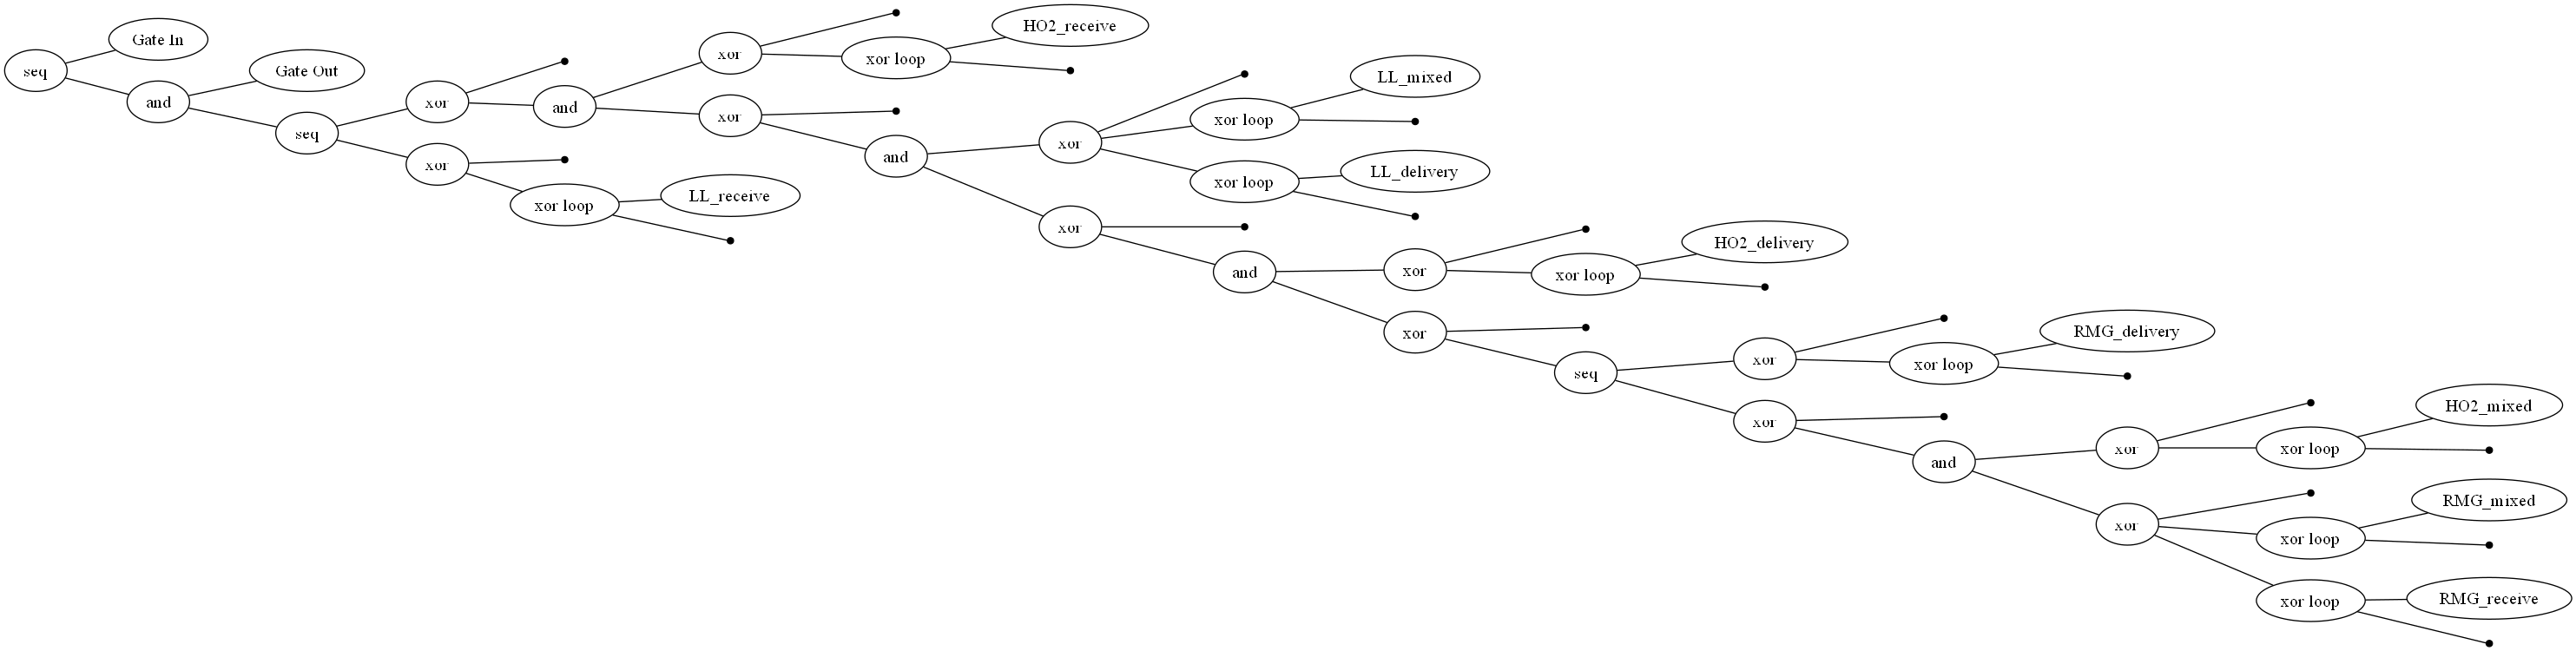
\includegraphics[width=\linewidth]{figures/discovery/process_tree.png}
    \subcaption{Process tree.}
    \label{fig:model_tree_theory}
\end{minipage}
\hfill
\begin{minipage}[t]{0.48\textwidth}
    \centering
    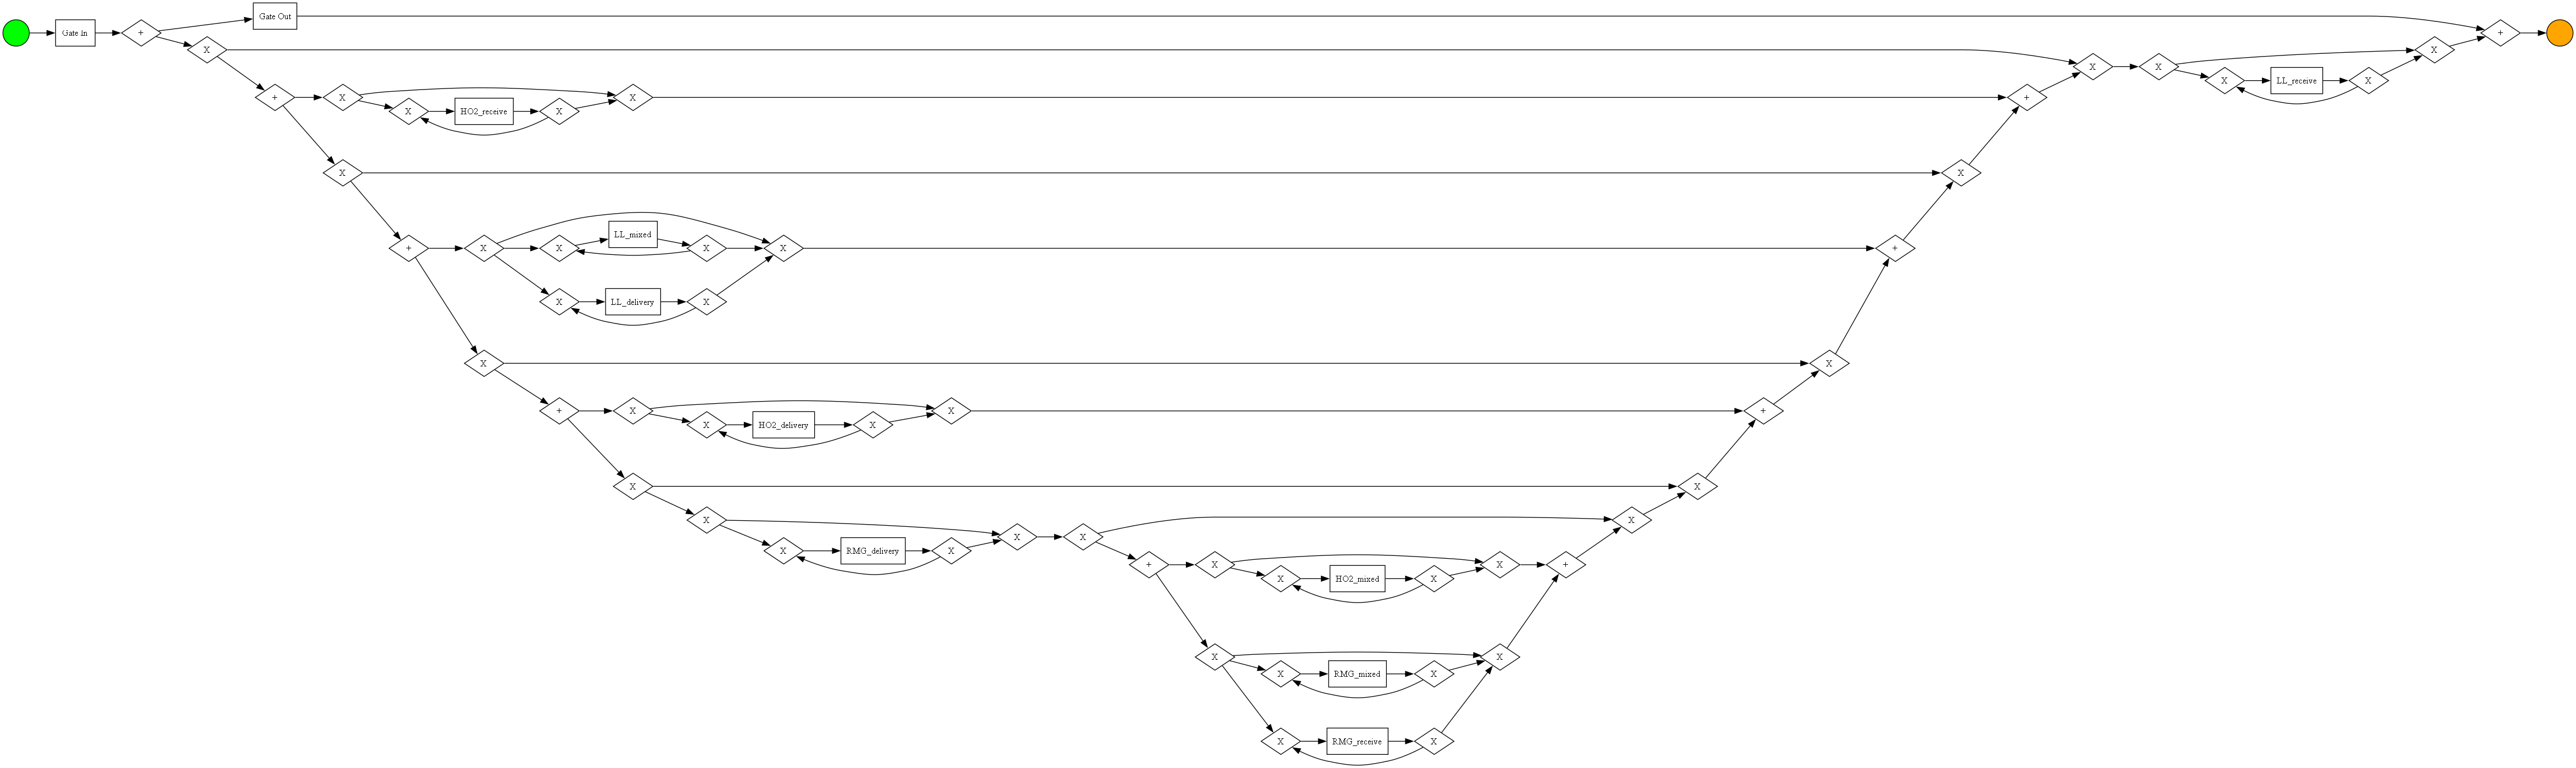
\includegraphics[width=\linewidth]{figures/discovery/bpmn.png}
    \subcaption{BPMN translation of the same process tree.}
    \label{fig:model_bpmn_theory}
\end{minipage}
\caption{Two representations of the same discovered control flow
(inductive miner on the CTB training log). The process tree exposes
the hierarchical operator structure; the BPMN translation preserves
the same behavior using the industry-standard graphical vocabulary.
Both models describe an identical set of allowed traces and are used
interchangeably in the process mining literature
\cite{PMvanDerAalst2016}.}
\label{fig:model_representations}
\end{figure}

\subsubsection{Conformance Checking}
While process discovery focuses on constructing process models, conformance checking focuses on comparing observed process executions with an existing process model \cite{aalst2012ConformanceChecking}. The objective is to identify deviations between the discovered model and the observed reality. Resulting deviations can indicate compliance violations, process inefficiencies, exceptional cases, or outdated process documentation. The quality of discovered process models is commonly evaluated using four criterias \cite{aalst2012ConformanceChecking,PMvanDerAalst2016}: 

\begin{itemize} \item \textbf{Fitness}: 
Measures how well the process model can reproduce the observed behavior in the event log. A model with high fitness allows most observed traces to be replayed without deviations.
\item \textbf{Precision}:
Measures how much additional behavior the model allows beyond the behavior observed in the event log. A precise model avoids allowing many unrealistic or unobserved execution paths. 
\item \textbf{Generalization}: 
Measures whether the model captures the underlying process behavior rather than only reproducing the exact traces contained in the event log. A model should therefore allow plausible behavior that was not necessarily observed in the available sample. 
\item \textbf{Simplicity}: 
Measures the complexity of the process model. Among models that describe the observed behavior sufficiently well, simpler models with fewer unnecessary elements and relations are generally preferred because they are easier to be interpreted and analysed. 
\end{itemize}

These criteria provide a balanced framework for evaluating process model quality and form the basis of many process-mining evaluation approaches. 

\paragraph{A*-based optimal alignment.}
\label{sec:astar_alignment_definition}
An alignment relates an observed trace to an executable run of a process
model. Formally, it is a sequence of three move types: a
\emph{synchronous move} consumes an event and fires a transition with the
same visible label; a \emph{log move} consumes an event without a
corresponding model transition; and a \emph{model move} fires a model
transition without consuming an observed event. A cost function normally
assigns zero cost to synchronous moves and positive, configurable costs
to deviations. An optimal alignment $\lambda^{\star}$ is therefore
\begin{equation}
\lambda^{\star}=\arg\min_{\lambda\in\Lambda(\sigma,N)} c(\lambda),
\end{equation}
where $\Lambda(\sigma,N)$ is the set of legal alignments between trace
$\sigma$ and process model $N$ \cite{aalst2012ConformanceChecking,
Adriansyah2011CostFitness}.

The qualifier ``A*-based'' refers to the search procedure, not to a
different kind of alignment. A* explores the product state space of the
current trace position and the current model state (for a Petri net, its
marking). It orders candidates by $f=g+h$, where $g$ is accumulated move
cost and $h$ is an admissible lower bound on the remaining cost. With an
admissible heuristic, the first complete solution is cost-optimal
\cite{Adriansyah2011CostFitness}. The resulting event--transition
correspondence supports conformance diagnostics and timestamp replay for
performance analysis \cite{aalst2012ConformanceChecking}; it does not
turn a model-derived enablement instant into an independently observed
timestamp.

\subsubsection{Process Enhancement} The Process Mining literature distinguishes three major categories of process mining techniques: process discovery, conformance checking, and process enhancement \cite{PMvanDerAalst2016}. The discovery creates a process model from event logs, conformance checking compares observed behavior with existing models and process enhancement then aims to improve existing process models using information extracted from event data. Enhancement includes different approaches. For example, performance information such as waiting times or activity durations can be projected onto a process model. Resource assignments, bottlenecks, and workload information can be incorporated to create richer process representations. Process enhancement can therefore enable process responsibles not only to understand how processes operate, but also identify opportunities for process improvement and optimization \cite{PMvanDerAalst2016}.

%%%%%%%%%%%%%%%%%%%%%%%%%%%%%%%%%%%%%%%%%%%%%%%%%%%%%%%%%%%%%%%%%%%%%% 
\section{Business Process Simulation} %%%%%%%%%%%%%%%%%%%%%%%%%%%%%%%%%%%%%%%%%%%%%%%%%%%%%%%%%%%%%%%%%%%%%% 

\subsection{Fundamentals of Business Process Simulation} 
Business Process Simulation (BPS) is an established analytical technique used to reproduce and analyze the dynamic behavior of business processes within a virtual environment. Rather than having to experiment directly on operational systems, organizations can build executable models that represent required process characteristics and repeatedly execute these models under controlled conditions. This allows process behavior to be observed without disturbing live operations \cite{BPSAalst2015}. Van der Aalst defines simulation as a flexible approach for analysing business processes and evaluating alternative operational scenarios. By recreating process executions under varying conditions, simulation can estimate process performance indicators such as throughput times, waiting times, resource utilization, service levels, and operational costs before changes have to be implemented in practice \cite{BPSAalst2015}. The primary purpose of simulation is the decision support. Business processes often run under uncertainty, dynamic resource interactions, and complex dependencies that make standard analytical evaluation difficult. Simulation provides a safe and cost-efficient environment for assessing operational modifications, while avoiding all the risks associated with real-world experimentation \cite{BPSAalst2015}. One of the most important applications of simulation is the so called \textit{what-if analysis}. What-if analyses evaluate how process performance changes under alternating assumptions or operational configurations. Typical examples include increasing the number of available resources, modifying routing rules, changing workload levels, or introducing new operational policies. By comparing simulation outcomes from different scenarios, decision makers can assess the expected consequences of proposed changes before implementation \cite{BPSAalst2015}. Because of its ability to represent dynamic process behavior and operational dependencies, simulation has become an established decision-support tool in fields such as manufacturing, healthcare, logistics, supply-chain management, and business process management. More recently, Process Mining research has increasingly integrated simulation based on observed event data, enabling simulation models to be discovered and calibrated directly from recorded process executions \cite{PMRozinat2009,Camargo2020}. 

\subsection{Business Process Simulation Models} 
A simulation model serves as a simplified representation of a real-world process. Although modeling approaches can vary, most business process simulation models consist of several fundamental perspectives that determine process behavior during simulation runs \cite{BPSAalst2015,PMRozinat2009}. 

\subsubsection*{Control Flow} 
The control-flow perspective describes the general behavioral structure of the process. It determines which activities exist, in which order they may occur, and which alternative execution paths are possible. In simulation models, the control-flow model serves as the structural backbone that governs the process execution. Commonly used representations include Petri nets, BPMN models, process trees, and workflow graphs \cite{PMvanDerAalst2016,BPSAalst2015}. 

\subsubsection*{Arrival Process} 
The arrival process defines how new process instances enter the system. In business processes, this typically corresponds to customer requests, orders, applications, service tickets, or other incoming work items. Arrival behavior is commonly represented through statistical distributions that describe the time between consecutive process initiations or arrivals. Since the incoming workload levels directly influence waiting times and resource utilization, realistic arrival modeling is essential for acurate simulation results \cite{BPSAalst2015,PMRozinat2009}. 

\subsubsection*{Resources} 
Resources represent the entities that execute process activities. Depending on the application domain, resources may correspond to employees, machines, vehicles, cranes or other terminal equipment. Resource models typically include information about availability, capacities, execution capabilities and multitasking abilities, working schedules, and allocation policies. Resource constraints are often important determinants of process performance because multiple process instances compete for limited resource capacity \cite{BPSAalst2015}. 

\subsubsection*{Activity Durations} 
The timing perspective describes how long activities require for their execution. Typical simulation models distinguish between processing times, waiting times, and overall case durations. Activity durations can be represented through probability distributions derived from historical observations. These temporal characteristics largely determine process performance and throughput behavior \cite{BPSAalst2015,PMRozinat2009}. 

\subsubsection*{Decision Logic} 
Business processes usually contain decision points where alternative execution paths can be selected. A Models learned decision logic determines how these routing decisions are made during simulation. Traditional simulation models employ static branching probabilities that specify how often a particular path is chosen. More advanced approaches model decisions as functions of contextual information, process attributes, or operational conditions at certain points in the path \cite{PMRozinat2009,mannhardt2023stochasticProcessesModelling}. 
\begin{sloppypar}
Together, control flow, arrivals, resources, timing information, and decision logic define the behavior of a simulation model. These perspectives form the foundation of both traditional manually developed simulation models and modern simulation-discovery approaches discussed later in this chapter. 
\end{sloppypar}


\subsection{Simulation-Based Decision Support} 
Container terminals operate in very dynamic environments characterized by fluctuating demand, limited resource capacity, and strong interdependencies between operational processes. Managers must continuously make decisions regarding equipment allocation, workforce planning, storage relocation strategies, truck appointment policies, and capacity utilization while maintaining uninterrupted terminal operations. Direct experimentation in a live terminal environment is often impractical because operational changes may negatively affect service quality, throughput, or customer satisfaction. As a consequence, simulation has become one of the most widely applied decision-support approaches in container terminal research \cite{Bruzzone2012,Kastner2021,Carboni2025}. By providing a virtual representation of terminal operations, simulation enables decision makers to evaluate operational alternatives before implementation. Typical applications include: 

\begin{itemize} 
    \item evaluation of truck appointment policies, 
    \item resource and workforce planning, 
    \item capacity planning and investment decisions, 
    \item yard layout and storage strategies, 
    \item yard crane allocation policies, 
    \item congestion analysis and bottleneck identification, 
    \item equipment scheduling and maintenance planning. 
\end{itemize} 

A core advantage of simulation is its ability to support what-if analyses. Alternative operational scenarios can be evaluated under identical conditions, allowing direct comparison of performance measures such as truck turnaround times, resource utilization, throughput, waiting times, and service levels. This capability is particularly valuable in container terminals because small operational changes frequently generate system-wide effects due to the strong interdependencies between gate operations, yard processes, and vessel handling activities \cite{CTSteenken2004,Bruzzone2012,Kastner2021}. For truck operations, simulation has been extensively applied to study the effects of Truck Appointment Systems (TAS), gate capacities, yard utilization, and equipment allocation strategies. Such analyses are usually terminal specific, but can support terminal operators in balancing efficiency improvements with operational robustness under uncertain workloads and changing operating conditions \cite{Bett2024,CTprocessMiningTAS2020}. 

\subsection{Simulation Model Calibration}
Calibration estimates or adjusts simulation parameters so that the
model represents the observed operating conditions. Typical tasks
include fitting arrival and duration distributions, estimating resource
capacities, and learning routing probabilities or context-dependent
decision rules from historical observations
\cite{PMRozinat2009,Camargo2020}. In simulation discovery, many of these
steps form part of the automated discovery procedure itself. Calibration
must nevertheless be distinguished from validation: agreement with the
data used to fit a model demonstrates in-sample fit, whereas an
independent assessment requires data that did not determine those
parameters. Section~\ref{sec:simulation_validation_background} develops
the corresponding verification and validation concepts.


%%%%%%%%%%%%%%%%%%%%%%%%%%%%%%%%%%%%%%%%%%%%%%%%%%%%%%%%%%%%%%%%%%%%%%%%%%%%%%%%%
\section{Simulation Discovery and Data-Aware Simulation} 
%%%%%%%%%%%%%%%%%%%%%%%%%%%%%%%%%%%%%%%%%%%%%%%%%%%%%%%%%%%%%%%%%%%%%%%%%%%%%%%%%

The previous sections established the main components of Business Process Simulation and the role of event logs in Process Mining. Simulation discovery connects these two perspectives by deriving executable simulation behavior directly from recorded process executions. Rather than introducing simulation parameters as manually specified assumptions, simulation-discovery approaches estimate them from event logs and integrate them into an executable process model \cite{PMRozinat2009,Camargo2020,simod2024}. The development of this research stream has progressively moved from the discovery of classical stochastic simulation parameters toward context-dependent and data-aware process behavior.

\subsection{From Simulation Discovery to Data-Driven Simulation} 

One of the foundational approaches to automatically derive simulation models from event logs was proposed by Rozinat et al. \cite{PMRozinat2009}. Their framework combines Process Mining and simulation by extracting several behavioral perspectives from historical executions, including control flow, temporal behavior, resource assignments, arrival characteristics, and routing probabilities.

Subsequent research extended this idea by refining the stochastic representation of process behavior. Solti et al. \cite{stochastikPetriNets2013Solti} investigate the discovery of stochastic Petri nets with arbitrary delay distributions, thereby integrating richer temporal behavior into formally discovered process models. Later, Camargo et al. \cite{Camargo2020} proposed a more automated framework for discovering executable Business Process Simulation models from event logs, including process structure, activity durations, resource pools, calendars, and arrival behavior. More recent frameworks such as Simod further systematise the automated discovery and calibration of simulation models from event data \cite{simod2024}.

A parallel branch researches uprising expressive generative models of process behavior. Camargo et al. \cite{Camargo2021} compare conventional data-driven process simulation with deep-learning-based generative models, illustrating that simulation discovery can move beyond separately fitted marginal distributions and toward models capable of learning more complex behavioral dependencies. This increased expressiveness, but at the same time also raises questions about transparency and configurability, which are discussed in Section~\ref{sec:explainable_simulation}.

The development can therefore be understood as a shift from extracting conventional simulation parameters from event logs towards learning increasingly enabled stochastic relationships between process state and simulated behavior \cite{PMRozinat2009,Camargo2020,Camargo2021}.


\subsection{Discovery of Simulation behavior} 

The simulation perspectives introduced in Section~\ref{sec:bps_models} remain the core objects of discovery, but the way they are represented has evolved considerably.

\subsubsection{Control-Flow and Stochastic Routing}

Early simulation-discovery approaches combined process discovery with stochastic information derived from observed executions \cite{PMRozinat2009}. While a discovered process model determines which activities may occur, stochastic weights determine how likely alternative paths actually are. Stochastic process discovery therefore extends purely structural process models with estimating the relative likelihood of alternative transitions \cite{stochastikPetriNets2013Solti,burke2020stochasticPD}.

The quality of the discovered control-flow structure stays important for simulation because the model defines the behavior that can be generated. Excessive generalisation may enable execution paths that were not observed or that are operationally implausible, whereas overly restrictive models may fail to represent legitimate process variability \cite{PMvanDerAalst2016,VinciDeLeoni2025Repair}. The balance between fitness and precision is therefore not only relevant for process discovery but also directly affects the behavioral space of the resulting simulator \cite{VinciDeLeoni2025Repair}.

\subsubsection{Temporal and Resource Behavior}

Simulation-discovery research has progressively moved from globally fitted distributions toward more differentiated temporal and resource models. Early approaches estimate execution times, waiting behavior, and resource characteristics from observed event-log distributions \cite{PMRozinat2009,stochastikPetriNets2013Solti}. More recent approaches additionally represent calendars, resource pools, allocation rules and heterogeneous resource behavior \cite{Camargo2020,BPSdifferentiatedResources2022}.

This development is particularly relevant because temporal behavior is rarely independent of the operational context. Execution and waiting times may vary with workload, resource availability, case characteristics or previous process behavior. Similarly, the probability of selecting a particular resource may depend on more than a static activity-resource mapping \cite{BPSdifferentiatedResources2022,Vinci2026prosit}. Recent simulation-discovery approaches therefore increasingly model these dimensions conditionally rather than as one global distribution per activity or resource.

\subsubsection{Arrival behavior}

Arrival processes have likewise evolved from globally fitted inter-arrival distributions toward context-dependent representations. Classical simulation-discovery approaches estimate inter-arrival times from historical case-start timestamps \cite{PMRozinat2009,Camargo2020}. More recent approaches can condition arrival behavior on temporal or contextual information, allowing the simulator to represent non-stationary workload patterns rather than assuming a single pooled arrival process \cite{Vinci2026prosit}. This distinction is important in operational settings where demand varies systematically across hours, weekdays, or operating periods.


\subsection{Data-Aware and Process-State-Aware Simulation}

A central limitation of classical stochastic simulation models is that routing probabilities and other behavioral parameters are often estimated globally. For example, if two alternative process paths occur with frequencies of 70\,\% and 30\,\%, a conventional stochastic model may assign these probabilities independently of the characteristics of the particular case. Such a representation captures how often alternatives occurred, but not why different process instances followed different paths \cite{PMRozinat2009,burke2020stochasticPD}.

Data-aware simulation addresses this limitation by conditioning stochastic behavior on process data. Mannhardt et al. \cite{mannhardt2023stochasticProcessesModelling} extend stochastic Petri nets with data-dependent transition weights, so that the probability of an enabled transition can depend on process variables instead of being represented by one global value. The resulting model therefore captures systematic differences between cases with different characteristics.

De Leoni et al. \cite{Vinci2023Inf.Activ.Prob} extend this idea through the concept of the \textit{process state}. Rather than conditioning decisions only on static case attributes, the process state may also describe information accumulated during the execution of the case, including process-variable values and the history of previously executed activities. Their results show that incorporating this richer representation of the current process state can improve the estimation of activity-firing probabilities compared with basic frequency-based branching probabilities.

The conceptual development can therefore be represented as:

\begin{center}
Static Branching Probabilities \\
$\downarrow$ \\
Stochastic Process Models \\
$\downarrow$ \\
Data-Dependent behavior \\
$\downarrow$ \\
Process-State-Aware Simulation
\end{center}

Recent work extends data awareness beyond routing behavior. López-Pintado et al. \cite{lopez2024} investigate the discovery and simulation of data-aware business processes more broadly, reflecting a shift toward simulation models in which multiple behavioral dimensions depend on process context rather than only on marginal historical frequencies.


\subsection{ProSiT as a Probabilistic Data-Aware Simulation Framework}

The ProSiT framework represents a recent development within this research direction \cite{Vinci2026prosit}. Instead of applying data awareness only to routing decisions, ProSiT models several simulation dimensions through probabilistic white-box predictors, including control-flow decisions, execution times, waiting times, resource selection, and arrival behavior.

The framework uses probabilistic decision trees to partition the available feature space and associates each resulting leaf with a local probability distribution. Simulation behavior can therefore differ between process contexts while remaining stochastic. This is conceptually different from both a conventional simulation model with one global distribution per parameter and a deterministic predictive model that returns a single point estimate.

An important distinction is required between different forms of contextual information. In the published ProSiT framework, simulation-parameter discovery can use trace attributes, execution history, resource information, temporal information, and workload-related features \cite{Vinci2026prosit}. This does not imply unrestricted support for arbitrary event-level attributes that change continuously during execution. The more general process-state perspective described by Mannhardt et al. \cite{mannhardt2023stochasticProcessesModelling} and de Leoni et al. \cite{Vinci2023Inf.Activ.Prob} therefore provides a broader conceptual framework than the particular feature representation currently implemented in ProSiT.

For this thesis, ProSiT is particularly useful because its level of contextual conditioning can be varied experimentally. The framework therefore makes it possible to test whether increasing model expressiveness actually translates into improved held-out simulation fidelity in the CTB truck process.


\paragraph{Configurable expressiveness in ProSiT.}

Two ProSiT configuration parameters are particularly relevant for the experimental design in Section~\ref{sec:simulation_discovery_methodology} \cite{Vinci2026prosit}:

\begin{itemize}
    \item \texttt{max\_depth\_tree} controls the maximum depth of the probabilistic decision trees used for conditional simulation behavior. Setting \texttt{max\_depth\_tree}$=0$ disables conditional tree-based modelling and yields an unconditional distribution-based configuration. Increasing the depth allows the model to distinguish more detailed combinations of contextual features, while also increasing model complexity and potential overfitting.

    \item \texttt{use\_workload\_features} determines whether workload-related features are made available to the waiting-time and resource-selection models. When enabled, these models can condition their behavior on the current operational workload and queue state in addition to the remaining contextual attributes.
\end{itemize}

These parameters define the comparison used later in this thesis between a distribution-based configuration, a data-aware configuration, and a data-aware configuration additionally enriched with workload information. Whether this increased expressiveness improves simulation fidelity is treated as an empirical question rather than assumed in advance.

%%%%%%%%%%%%%%%%%%%%%%%%%%%%%%%%%%%%%%%%%%%%%%%%%%%%%%%%%%%%%%%%%%%%%%%%%%%%%%%%%
\section{Explainable and White-Box Simulation}
%%%%%%%%%%%%%%%%%%%%%%%%%%%%%%%%%%%%%%%%%%%%%%%%%%%%%%%%%%%%%%%%%%%%%%%%%%%%%%%%%%

\subsection{Explainability in Simulation-Based Decision Support}
Business Process Simulation is becoming increasingly popular to support operational and strategic decision making. Simulation results are often the basis for resource-allocation strategies ans decisions, process redesign initiatives, capacity planning, and investment evaluations. Therefore decision makers have to be able to understand why a simulation model produces a particular outcome and how simulation behavior changes when process parameters are modified. Traditional Business Process Simulation models are transparent from design \cite{BPSAalst2015}. Their control-flow structures, routing probabilities, resource allocations, and time assumptions are manually specified and can therefore be analysed and modified by developers and domain experts. That way, simulation users can directly understand the assumptions underlying the generated simulation results \cite{BPSAalst2015}. Recent advances in simulation discovery increasingly employ machine-learning and deep-learning techniques to improve the simulation accuracy. These approaches learn behavioral patterns directly from historical event data and often outperform manually calibrated models in terms of predictive capabilities \cite{Camargo2020, Camargo2021}. However, the resulting models frequently behave as black-box systems. While they can generate more accurate predictions, the internal decision mechanisms that govern the simulation behavior, are not readily interpretable by developers or human analysts. This creates a tension between predictive accuracy and explainability. Black-box simulation models therefore may successfully reproduce historical process behavior while simultaneously limiting the analyst's ability to understand why particular routing decisions, waiting times, or resource allocations are generated. Consequently, the simulation model becomes difficult to inspect, configure, validate, and trust for operational decision support \cite{runtimeIntegration2024}. The explainability problem becomes especially relevant for what-if analyses. Business Process Simulation is not only intended to reproduce observed behavior but also to evaluate hypothetical future scenarios. Devlopers have to be able to intentionally modify process parameters, resource settings or decision rules. In black-box simulation approaches, the underlying behavioral logic is often inaccessible, making it difficult to assess whether the simulated reactions to process changes are realistic and trustworthy \cite{runtimeIntegration2024}. To address these limitations, recent research has started investigating explainable simulation models that combine the predictive capabilities of machine-learning approaches with transparent and interpretable decision logic. The goal is not only to reproduce process behavior accurately but also to expose the reasoning mechanisms that determine simulation outcomes. Explainability therefore becomes an important prerequisite for trustworthiness, configurability, and practical adoption of data-driven simulation models.

\subsection{Probabilistic White-Box Simulation Models} 
The concept of white-box simulation emerged as a response to the increasing reliance on opaque machine-learning models for simulation parameter discovery. White-box simulation models aim to make behavioral decisions explicitly visible and interpretable while maintaining a high degree of simulation accuracy. A key motivation behind white-box simulation is that business analysts must be able to inspect, understand, and modify the simulation behavior that drives decision-support outcomes. Unlike black-box predictors, white-box approaches expose the discovered decision rules and allow analysts to evaluate the causal relationships that influence simulation parameters. An important step towards explainable simulation is represented by the Runtime Integration of Machine Learning and Simulation (RIMS) framework proposed by Meneghello et al. \cite{runtimeIntegration2024}. RIMS combines traditional discrete-event simulation with predictive machine-learning models at runtime. The authors explicitly argue that purely deep-learning-based simulation approaches suffer from limited explainability and restricted support for what-if analyses. By maintaining an explicit simulation model while integrating learned predictions during execution, RIMS seeks to combine simulation transparency with data-driven prediction capabilities \cite{runtimeIntegration2024}. More recently, Vinci et al. introduced the ProSiT framework (\textit{PROcess SImulation Tool}), which represents one of the first dedicated white-box simulation-discovery approaches \cite{Vinci2026prosit}. ProSiT extends data-aware simulation discovery by replacing opaque prediction mechanisms with probabilistic decision trees. These trees are used to represent multiple simulation dimensions including: \begin{itemize} \item control-flow decisions, \item activity execution times, \item waiting times, \item resource assignment behavior, \item arrival processes. \end{itemize} The central idea of ProSiT is that simulation behavior should remain directly interpretable. Instead of producing predictions through hidden neural-network representations, behavioral rules are exposed explicitly in the form of decision-tree structures. Analysts can therefore inspect, understand, and modify the conditions influencing simulation behavior \cite{Vinci2026prosit}. An additional contribution of ProSiT is the integration of uncertainty through probabilistic decision trees. Traditional decision trees often generate deterministic predictions. In contrast, probabilistic decision trees capture distributions of possible outcomes and thereby preserve the stochastic nature required for realistic process simulation \cite{Vinci2026prosit}. This is particularly important because simulation models aim not only to reproduce average behavior but also the variability observed in real operational environments. Experimental evaluations presented by Vinci et al. indicate that probabilistic white-box models can achieve simulation accuracy comparable to, and in some cases exceeding, alternative black-box approaches while simultaneously improving interpretability and configurability \cite{Vinci2026prosit}. Furthermore, the framework enables process analysts to directly edit discovered rules and evaluate modified decision scenarios without retraining complex machine-learning models. Despite these promising results, research on white-box simulation remains at an early stage. Current evidence is largely limited to benchmark datasets and business-process environments investigated by the authors themselves. Large-scale empirical evaluations across different domains remain scarce. In particular, little evidence currently exists regarding the behavior of white-box simulation models in highly dynamic cyber-physical systems such as container terminals. Moreover, explainability itself remains difficult to quantify. While decision trees are generally considered more transparent than neural networks, there is currently no universally accepted framework for measuring the practical interpretability of simulation-discovery models. Existing evaluations primarily focus on simulation accuracy, leaving questions related to user trust, decision-support quality, and operational usefulness largely unexplored. Consequently, white-box simulation should not yet be regarded as a mature solution to the explainability challenge. Rather, it represents an emerging research direction that attempts to balance three competing objectives: 

\begin{enumerate} 
\item simulation accuracy, 
\item simulation explainability, 
\item simulation configurability. 
\end{enumerate} 

The ProSiT framework currently represents one of the most comprehensive realizations of this vision and serves as the methodological foundation for the simulation approach investigated in this thesis \cite{Vinci2026prosit}.

%%%%%%%%%%%%%%%%%%%%%%%%%%%%%%%%%%%%%%%%%%%%%%%%%%%%%%%%%%%%%%%%%%%%%%%%%%%%%%%%%%%
For terminological precision, the relationships exposed by such learned
rules are statistical associations conditional on the training data and
model specification. Their visibility supports inspection and deliberate
configuration, but does not by itself establish causal effects.

%%%%%%%%%%%%%%%%%%%%%%%%%%%%%%%%%%%%%%%%%%%%%%%%%%%%%%%%%%%%%%%%%%%%%%%%%%%%%%%%%%%
\section{Simulation Verification, Validation, and Trustworthiness}
\label{sec:simulation_validation_background}
The central validation question is not whether a simulator is merely
executable, but whether it is sufficiently credible for its intended
use. This qualification is essential: a model may be adequate for
reproducing historical truck turnaround distributions while remaining
inadequate for predicting the effect of an intervention outside the
range of the observed data \cite{Sargent2013Validation,BPSAalst2015}.
Automatically discovered simulation models do not remove this
requirement. They replace some manual assumptions with assumptions about
event-log semantics, discovery algorithms, data attributes and fitted
distributions, all of which require examination.

\subsection{Foundational Distinction Between Verification and Validation}

Sargent separates several questions that are often conflated under the
single term \emph{validation} \cite{Sargent2013Validation}.
\emph{Conceptual-model validity} asks whether the theories, assumptions
and logical relationships in the conceptual model are reasonable for
the intended purpose. \emph{Computerized-model verification} asks
whether that conceptual model has been implemented correctly.
\emph{Data validity} concerns whether the data used to construct,
calibrate and evaluate the model are adequate. Finally,
\emph{operational validity} asks whether the computerized model's
output behaviour is sufficiently accurate over the domain in which the
model is intended to be used. Historical-data validation---running the
model under historical input conditions and comparing its output with
observed system data---is one technique for assessing operational
validity \cite{Sargent2013Validation}.

Table~\ref{tab:validation_evidence_types} maps these distinctions to the
type of evidence needed in an automatically discovered BPS study. The
categories are complementary rather than interchangeable. For example,
a low event-log distance is evidence of operational fidelity, but it
cannot show that a timestamp proxy has the correct physical meaning or
that the simulator implemented a resource constraint as intended.

\begin{table}[htbp]
\centering
\caption{Validation questions and corresponding evidence in an
event-log-discovered simulation study, based on Sargent's framework
\cite{Sargent2013Validation}.}
\label{tab:validation_evidence_types}
\begin{tabular}{p{0.23\textwidth}p{0.29\textwidth}p{0.39\textwidth}}
\toprule
\textbf{Question} & \textbf{Validity concept} & \textbf{Typical evidence} \\
\midrule
Is the abstraction defensible? & Conceptual-model validity &
Domain review of case boundaries, event semantics, resource meanings
and physical constraints \\
Was the abstraction implemented correctly? & Computerized-model
verification & Unit and integration tests, structural contracts,
reproducible seeds and parameter-provenance checks \\
Are discovery and evaluation data suitable? & Data validity &
Event-log quality checks, timestamp semantics, leakage prevention and a
training/test separation \\
Does the model reproduce observed behaviour? & Operational validity &
Comparison of simulated and held-out real logs across multiple process
perspectives and stochastic replications \\
Does a scenario predict the true intervention effect? & Predictive
validity outside the historical regime & Intervention observations,
controlled field evidence or additional domain-supported sensitivity
analysis \\
\bottomrule
\end{tabular}
\end{table}

This distinction also clarifies the scope of this thesis. The
real-versus-simulated event-log comparison is a form of held-out
historical-data or operational validation. The event-log construction
and the physical RMG capacity constraint contribute data- and
conceptual-validity evidence, while executable case contracts and
provenance checks contribute verification evidence. None of these alone
proves that every what-if response is the true causal response of the
terminal.

\subsection{From Historical Logs to Operational Validation}

Process Mining provides a natural representation for historical-data
validation because both the observed system and the simulator can be
represented by event logs. Rozinat et al. established an early version
of this principle: they discover control-flow, data, performance and
resource perspectives, integrate them into a coloured Petri-net
simulation model, simulate a second event log, and analyse how well that
generated log approximates the characteristics of the original log
\cite{PMRozinat2009}. This is stronger than checking whether the
discovered model can execute; it evaluates whether its generated
behaviour resembles recorded behaviour.

Camargo et al. formalise the same idea as an optimisation objective.
Candidate BPS configurations generate event logs and hyperparameter
optimisation searches for the configuration that maximises similarity
to observed log behaviour \cite{Camargo2020}. Their later comparison of
data-driven simulation and deep generative models further demonstrates
why quality must not be inferred from trace frequencies alone:
conventional data-driven simulators may reproduce activity sequences
and their frequencies while performing worse on temporal dynamics
\cite{Camargo2021}.

The implication is that operational fidelity is multi-dimensional.
Relevant perspectives include control flow, activity and case timing,
case arrivals, congestion and resource behaviour. A model can be close
to the real log in one perspective and far away in another; collapsing
all discrepancies into one number can therefore hide the mechanism
that is incorrectly represented
\cite{ChapelaCampa2023Trust,Chapela2025SimQuality}.

\subsection{Multi-Perspective Event-Log Comparison}

Chapela-Campa et al. provide the validation framework that most closely
matches the evaluation problem of this thesis
\cite{ChapelaCampa2023Trust,Chapela2025SimQuality}. Their starting point
is that the true BPS model is normally unavailable and that different
simulation engines use incomparable internal formats. They therefore
evaluate a model indirectly as a generator: multiple logs generated by
the BPS model are compared with an actual event log that was not used
to construct the model. The framework separates control-flow, temporal
and congestion perspectives and reports a measure for each instead of
claiming that one aggregate score represents overall model quality.
The measures are evaluated using controlled perturbations and by
comparing alternative automatically discovered BPS models, showing that
perspective-specific measures can identify the source of a discrepancy
\cite{Chapela2025SimQuality}.

\subsubsection{Control-Flow Perspective}

Control-flow output quality asks whether the simulator generates
activity sequences and sequence frequencies resembling the observed
process. It is distinct from replay fitness of a control-flow model:
fitness asks whether real traces are allowed by the model, whereas
output validation asks which traces the stochastic simulator actually
generates and with what frequency.

Stochastic conformance work applies transport distances to probability
distributions over traces or other behavioural abstractions
\cite{leeman2013EarthMovers}. Chapela-Campa et al. instead define two
simulation-oriented log distances \cite{ChapelaCampa2023Trust,
Chapela2025SimQuality}. Control-Flow Log Distance (CFLD) computes the
normalised Damerau--Levenshtein distance between trace pairs and uses
the Hungarian algorithm to find the minimum-cost one-to-one matching
between the two logs. CFLD therefore compares complete traces; it is not
merely a comparison of variant-frequency vectors. Because this matching
is computationally expensive, N-Gram Distance (NGD) compares normalised
frequencies of local activity subsequences. NGD is scalable and detects
local ordering differences, although it deliberately loses some
complete-trace information.

This thesis does not claim to implement the full Chapela-Campa metric
suite. Its structural evidence combines held-out Petri-net conformance,
explicit case-language contracts and yard-activity frequency error.
These measures answer the CTB-specific structural questions, while the
Chapela-Campa framework supplies the rationale for keeping structural
evidence separate from temporal fidelity.

\subsubsection{Temporal Perspective}

Identical or similar traces do not imply similar process performance.
Temporal validation considers whether the simulator reproduces when
events occur, how cases progress after arrival and how long activities
and complete cases take. Camargo et al. show empirically that a
generative model may represent control-flow frequencies adequately yet
miss temporal dynamics \cite{Camargo2021}.

The Chapela-Campa framework distinguishes three event-distribution
measures \cite{ChapelaCampa2023Trust,Chapela2025SimQuality}.
\emph{Absolute Event Distribution} (AED) compares event counts across
absolute calendar-time bins; \emph{Circadian Event Distribution} (CED)
compares recurring weekday and hour-of-day patterns; and
\emph{Relative Event Distribution} (RED) offsets timestamps by each
case's arrival and compares its temporal progression. Thus AED and RED
mean \emph{event distribution}, not absolute or relative error
distance. For end-to-end performance, Cycle Time Distribution (CTD)
compares the empirical distributions of complete case durations.

The CTB evaluation uses more directly interpretable distributions at
the level of its research questions: inter-arrival time, per-activity
yard service time, model-derived pre-service delay and case turnaround
time. Reporting complete distributions rather than only their means is
important because equal averages can conceal differences in dispersion,
skewness or tails. Per-activity results additionally prevent common RMG
events from concealing weaker fidelity for less frequent yard
activities.

\subsubsection{Arrival and Congestion Perspectives}

Congestion is a system-level consequence of the interaction between
demand, service requirements and resource availability. It cannot be
validated from activity-duration marginals alone. Chapela-Campa et al.
use Case Arrival Rate (CAR) to compare binned arrival counts and shapes,
and CTD to compare the second major congestion component, the length of
time cases remain in the system
\cite{ChapelaCampa2023Trust,Chapela2025SimQuality}. An arrival model can
therefore be temporally unrealistic even if it generates the correct
total number of cases.

This issue is central at CTB: truck demand determines competition for
yard resources, and simultaneous arrivals are meaningful consequences
of the minute-resolved source data. The evaluation consequently reports
inter-arrival distance, simultaneous-arrival share and arrivals per
elapsed hour alongside turnaround and yard-service distributions.
These measures do not directly observe a physical queue; they assess
whether the generated workload and its resulting temporal behaviour
match what the available event log can identify.

\subsubsection{Wasserstein Distance}

For two one-dimensional distributions $F$ and $G$ with finite first
moments, the first Wasserstein distance can be written as
\begin{equation}
    W_1(F,G)=\int_{-\infty}^{\infty}|F(x)-G(x)|\,\mathrm{d}x .
\end{equation}
It has the optimal-transport interpretation of the minimum cost of
moving probability mass from one distribution to the other. For
durations measured in minutes, $W_1$ is also expressed in minutes,
which gives the discrepancy an operational scale.

Earth Mover's Distance (EMD) is closely related, but the terms should
not be treated as universally interchangeable. In the formulation used
by Chapela-Campa et al., EMD may compare time series with unequal total
mass and penalise the creation of missing mass, whereas first
Wasserstein distance assumes equal normalised mass
\cite{ChapelaCampa2023Trust,Chapela2025SimQuality}. For empirical
probability distributions with unit mass, the formulations coincide.
In Process Mining, related transport distances have also been used for
stochastic conformance checking over behavioural distributions
\cite{leeman2013EarthMovers}. In this thesis, the term \emph{EMD} for
service, inter-arrival and turnaround samples denotes the
one-dimensional $W_1$ distance between empirical distributions.

\subsubsection{Kolmogorov--Smirnov Statistic}

The two-sample Kolmogorov--Smirnov (KS) statistic is the maximum
vertical difference between the empirical cumulative distribution
functions of the simulated and observed samples
\cite{Massey1951KS}:
\begin{equation}
    D_{n,m}=\sup_x
    \left|F_{n,\mathrm{sim}}(x)-F_{m,\mathrm{real}}(x)\right|.
\end{equation}
Unlike $W_1$, it is dimensionless and bounded by zero and one. The two
statistics are complementary: $W_1$ measures integrated displacement
on the operational scale, while KS reports the largest local CDF gap.
The KS statistic can be accompanied by a hypothesis-test $p$-value, but
that $p$-value answers a different question from practical fidelity.
With large event logs, small and operationally unimportant differences
can be statistically significant. The magnitude of the statistic and
the distributional plots must therefore be interpreted separately from
null-hypothesis rejection.

\subsubsection{Additional Requirements for Data-Aware Discovery}

A data-aware simulator conditions behaviour on case attributes, process
state or workload information rather than using only global
distributions and branching frequencies
\cite{Vinci2023Inf.Activ.Prob,lopez2024,Vinci2026prosit}. This adds a
validation layer. First, every predictor used at a simulated decision
point must be available at that point; attributes computed from a later
outcome create target leakage even if aggregate log similarity is high.
Second, discovery and model selection must be separated from the final
test log. Third, the generated log must satisfy process and domain
invariants that aggregate distances may overlook.

White-box rules help because their split conditions and leaf
distributions can be inspected and deliberately modified
\cite{Vinci2026prosit}. Interpretability, however, is not equivalent to
validity or causality. A readable rule may encode a spurious association,
and two differently specified models may reproduce the same marginal
distribution. Validation should therefore combine held-out output
fidelity with rule inspection, leakage checks, structural contracts,
domain constraints and sensitivity analysis. This is particularly
important for the CTB application, where timestamp fields are
operational proxies and a resource label does not necessarily denote a
physically interchangeable crane or storage position.

\subsubsection{Stochastic Replication and Confidence Intervals}

A BPS model is a stochastic generator. One fixed model can generate
many possible event logs, whereas the real test log is only one observed
realisation. A single simulated log therefore confounds model fidelity
with the random draws of that run. Chapela-Campa et al. address this
problem directly: they generate $K$ logs from $K$ simulation runs,
match their case count and start point to an actual test log that was
not used for model construction, compare every generated log with that
test log, and construct confidence intervals for each perspective-
specific distance \cite{ChapelaCampa2023Trust}. Their controlled
evaluation uses $K=10$ replications and reports means and 95\,\%
intervals.

This design is consistent with classical simulation-output analysis,
where independent replications with different random-number streams
provide observations for estimating a mean and its Monte-Carlo
uncertainty \cite{Law2015Simulation}. For replication-level values
$x_1,\ldots,x_N$, a two-sided Student-$t$ interval is
\begin{equation}
    \bar{x}\ \pm\
    t_{0.975,N-1}\frac{s}{\sqrt{N}},
\end{equation}
where $s$ is the sample standard deviation across replications.

The interpretation of this interval must remain narrow. Conditional on
one frozen discovered parameter bundle and one fixed real test log, it
quantifies the variability caused by simulation sampling. It does not
include event-log sampling uncertainty, input-distribution estimation
uncertainty, alternative discovery outcomes, measurement error or
uncertainty about the correctness of a what-if response. Those require
additional resampling, repeated discovery, sensitivity experiments or
external domain evidence. Chapter~\ref{chp:experiments_and_framework}
uses this conditional Monte-Carlo interpretation for its ten-seed
protocol.

\subsection{Trustworthiness and the Boundary of Historical Validation}

Historical fidelity is necessary for a simulator that claims to
represent an existing process, but it is not sufficient for unrestricted
decision support. Chapela-Campa et al. explicitly identify this limit:
comparison with an original event log assesses replication of the
\emph{as-is} process, not the accuracy of predictions after a process
change \cite{ChapelaCampa2023Trust,Chapela2025SimQuality}. Similarly,
Sargent's purpose-relative view implies that evidence collected in one
operating region cannot automatically validate use in another
\cite{Sargent2013Validation}.

Trustworthiness is therefore an evidence bundle rather than another
single metric. It includes data and conceptual validity, verified
implementation, held-out multi-perspective fidelity, reproducibility,
transparent assumptions, stochastic robustness, domain review and
clear limits on extrapolation. ProSiT contributes inspectable and
configurable probabilistic rules \cite{Vinci2026prosit}; recent applied
work shows how discovered simulation models can be connected to a real
resource-allocation problem \cite{Hospital2026Vinci}. These properties
make validation and scenario discussion more accessible, but neither
white-box structure nor a successful application substitutes for
intervention-specific evidence.

Accordingly, this thesis does not claim to solve the general
trustworthiness problem of simulation discovery. It contributes a
container-terminal case study: the model is tested against an unseen
historical period, across structural, temporal and arrival perspectives,
with repeated stochastic runs and explicit domain constraints. Scenario
results are interpreted as conditional consequences of the documented
model assumptions, not as experimentally established causal effects.

\subsection{Research Gap}

Container terminals represent highly dynamic and resource-constrained operational environments characterized by complex interactions between truck processes, yard operations, storage systems, and handling equipment. As a result, simulation has become one of the most widely used analytical methods for supporting operational decision making in container terminal management \cite{Bruzzone2012,Kastner2021,Carboni2025}. Despite this extensive use of simulation, most container terminal simulation models continue to be developed manually. Model construction, calibration, and maintenance require substantial modelling effort and domain expertise, limiting scalability and practical applicability in rapidly changing operational environments \cite{PMRozinat2009}. Simulation discovery addresses this limitation by automatically generating simulation models from event logs. Over the past decade, significant advances have been achieved in the discovery of simulation parameters, data-aware decision logic, and automated model construction \cite{Camargo2020,simod2024,Vinci2026prosit}. More recently, data-aware simulation approaches demonstrated that contextual information and process-state representations can substantially improve simulation accuracy compared to traditional branching probabilities \cite{mannhardt2023stochasticProcessesModelling,Vinci2023Inf.Activ.Prob}. In parallel, white-box simulation approaches such as ProSiT introduced interpretable probabilistic decision models that aim to improve transparency and configurability while maintaining strong predictive performance \cite{Vinci2026prosit}. However, existing empirical evaluations have primarily been conducted in healthcare, administrative, and generic business-process environments. To date, there is limited evidence regarding the applicability and behavior of simulation-discovery approaches within large-scale container terminal operations. Furthermore, the increasing complexity of data-aware and decision-aware simulation models raises unresolved questions concerning: \begin{itemize} \item the robustness of automatically discovered simulation models, \item their trustworthiness for operational decision support, \item their ability to reproduce congestion effects and workload dynamics, \item the practical value of white-box simulation in complex logistics environments. \end{itemize} This thesis does not aim to provide a general answer to these broader research challenges. Rather, it contributes an empirical case study within the context of truck-handling operations at the HHLA Container Terminal Burchardkai (CTB). By evaluating simulation-discovery approaches in a real-world container terminal environment, the thesis provides evidence regarding their applicability, strengths, and limitations in a domain that has received comparatively little attention within the existing simulation-discovery literature.


    \chapter{Case Study and Data Engineering}
\label{chp:case_study_and_data}

This chapter documents the operational context in which the data-aware
simulation is discovered and the execution pipeline that turns raw
operational records into a simulation-ready event log. The chapter is
dedicated to only outline the design, therefore no models are fitted, no hypotheses are tested,
and no experimental parameters are chosen yet. Its prpose is to establish the
data foundation on which every subsequent claim in
Chapters~\ref{chp:experiments_and_framework}
and~\ref{chap:results} builds on, so that these later claims and results can be analysed against their exact input.

Section~\ref{sec:cs_environment} introduces the HHLA Container Terminal
Burchardkai (CTB) in Hamburg, Germany, the truck-handling scope of the study and the data
sources that feed the event-log engineering pipeline.
Section~\ref{sec:event_log_engineering} describes the multi-stage
transformation that produces the final event log, including
lifecycle-timestamp reconstruction and the derivation of case-level
context attributes required by the ProSiT simulation framework
\cite{Vinci2026prosit}. The chapter closes with a summary of the final
event-log characteristics that are used as input to the
train/test split defined in
Section~\ref{sec:train_test_split}.

%%%%%%%%%%%%%%%%%%%%%%%%%%%%%%%%%%%%%%%%%%%%%%%%%%%%%%%%%%%%%%
\section{Case Study Environment}
\label{sec:cs_environment}
%%%%%%%%%%%%%%%%%%%%%%%%%%%%%%%%%%%%%%%%%%%%%%%%%%%%%%%%%%%%%%

    \subsection{HHLA Container Terminal Burchardkai}

    The case studys envorinment is the HHLA Container Terminal Burchardkai
    (CTB), one of Europe's largest container terminals, located in the
    Port of Hamburg. CTB handles approximately 2.6 million TEU
    (Twenty-foot Equivalent Units) annually across 315 hectares
    \cite{hhla2025}.

    \textbf{Truck Process Scope:} External trucks visit CTB to deliver
    or receive containers. The process comprises:
    \begin{enumerate}
        \item \textbf{Gate In}: Truck registers at the entry gate.
        \item \textbf{Container handling}: Rail-Mounted Gantry cranes
              (RMGs), Van Carriers (VC) or manual operators (HO2) load
              or unload containers at storage blocks.
        \item \textbf{Gate Out}: Truck exits the terminal.
    \end{enumerate}

    The CTB environment in this project comes with several resource-constrains. Located between the waterside and the landside, 22 RMG storage blocks (T06--T27) are operating and serving both ends simulataniously with a maximum of 3 automatic Gantry Cranes in parallel. Additionally the CTB has two specialised areas. An empty-container depot (In operational terms also called "MT" or "LL" - in German for "Leerlager") and a manually operated yard area (In operational terms also called HO2). The Terminal Gate consists of 16 lanes half of which built for incoming trucks, the other half for outgoing trucks. The amount of operated gates per day and shift differs, depending on the resource planing by the terminal management. 
   
    \subsection{Data Sources}
    \label{sec:cs_data_sources}

    The operational data used in this thesis originates from several
    information systems that support day-to-day terminal operations.
    Historically, the information-system landscape at CTB evolved
    organically, resulting in a heterogeneous environment in which
    different systems manage distinct aspects of terminal operations,
    orchestrated by a Terminal Operating System. The primary data
    sources for this study are:

    \begin{itemize}
        \item \textbf{ITS schedule (scheduling system)} — records truck
              visit schedules, including timestamps for each operational
              step (gate-in time, ready time at a handling point, order
              fulfilment time, gate-out time).
        \item \textbf{Report system} — captures stage-level execution
              data, including gate entry times, exchange-area
              assignments and container transaction records, bridging
              yard operations and container master data.
        \item \textbf{Yard management system} — snapshots every four
              hours of all yard block capacities and utilisation rates.
        \item \textbf{Container master data} — container-level details
              (size, type, hazardous material, dwell time, inbound and
              outbound carrier).
    \end{itemize}

    These systems generate independent data pools with different
    identifier schemes, requiring the data-integration procedure
    described in Section~\ref{sec:event_log_engineering}. Historical
    data from March and April 2026 (8 weeks) was extracted, covering
    approximately 104,000 truck visits.

    \textbf{Data volume:}
    \begin{itemize}
        \item 113,466 container move events,
        \item 104,000 truck visits,
        \item 336 yard-state snapshots for (8 weeks $\times$ 7 days $\times$
              6 snapshots per day).
    \end{itemize}

%%%%%%%%%%%%%%%%%%%%%%%%%%%%%%%%%%%%%%%%%%%%%%%%%%%%%%%%%%%%%%%%%%%%%%%%%
\section{Event Log Engineering}
\label{sec:event_log_engineering}
%%%%%%%%%%%%%%%%%%%%%%%%%%%%%%%%%%%%%%%%%%%%%%%%%%%%%%%%%%%%%%%%%%%%%%%%%

Event-log engineering is the first stage of the experimental pipeline.
The objective is to construct an integrated, process-oriented event log
from the raw operational data that satisfies the requirements of both
process mining and data-aware simulation while retaining as much
operational context as possible. This section describes the pipeline
stage by stage.

\subsection{Raw Data Sources and Preparation}

\subsubsection{ITS Schedule Data}

The ITS scheduling system provides the core scheduling data for the
truck operations reconstructed in this thesis. Each record represents
one activity instance within a truck visit and carries the following
key attributes:

\begin{itemize}
    \item \texttt{FAHRPLAN\_UID} — unique identifier for the truck visit
          (case ID).
    \item \texttt{LKW\_KENNZEICHEN} — truck license plate number.
    \item \texttt{ANLAUFPUNKT\_HALTESTELLE} — exchange area identifier
          (e.g.\ T20, LL, VC).
    \item \texttt{FP\_ZEITPUNKT\_ERSTELLUNG} — timestamp when the
          schedule entry was created (gate-in time).
    \item \texttt{ALP\_ZEITPUNKT\_BEREITMELDUNG} — timestamp when the
          activity became ready for execution (enabled time).
    \item \texttt{ALP\_ZEITPUNKT\_ERFUELLUNG} — timestamp when the
          activity was completed.
    \item \texttt{FP\_ZEITPUNKT\_GATEOUT} — timestamp when the truck
          exited the terminal.
\end{itemize}

All timestamp fields are parsed into standardised \texttt{datetime}
objects using \texttt{pandas} with the format
\texttt{\%d.\%m.\%Y~\%H:\%M}. Invalid or missing timestamps are flagged
for removal during the cleaning phase.

\subsubsection{Report System Data}

The report system provides complementary stage-level execution data,
completing the details for gate-entry events, and it links each
container number to the specific truck visit at a yard handling point.
Key attributes are:

\begin{itemize}
    \item \texttt{TruckVisitGkey} — unique truck-visit identifier used
          for cross-system matching.
    \item \texttt{TruckLicenseNbr} — truck license plate.
    \item \texttt{CallupTime} — timestamp when the truck physically
          entered the terminal.
    \item \texttt{StageStartTime} — timestamp when the activity became
          ready for execution (enabled time).
    \item \texttt{StageId} — stage identifier
          (e.g.\ \texttt{OCR}, \texttt{Gate-In}, \texttt{yard},
          \texttt{Exit}).
    \item \texttt{TruckExchangeArea} — visited handling point in the
          yard for a specific container.
    \item \texttt{TranCtrNbr} — container number associated with the
          transaction.
    \item \texttt{UnitInboundCarrierId} — inbound carrier identifier
          (truck plate, vessel voyage number or train ID).
    \item \texttt{UnitOutboundCarrierId} — outbound carrier identifier
          (truck plate, vessel voyage number or train ID).
\end{itemize}

A container is considered ``picked up'' or ``delivered'' by a truck if
the corresponding inbound or outbound carrier identifier resolves to a
truck. The report system uses detailed handover-lane codes for the
exchange area; these must be mapped to the higher-level operational
zones used by the scheduling system. Specifically, all exchange areas
beginning with ``HP'' (\textit{Hochpalette}) are mapped to ``LL''
(\textit{Leerlager}) to align with the schedule system's terminology.
The mapping is implemented in
\texttt{002\_Prep\_area\_mapping\_report.py}.

\subsubsection{Container Master Data}

Container-level attributes are extracted from the container master data
and linked to events via the matched \texttt{container\_id}:

\begin{itemize}
    \item \textbf{Container size} — TEU equivalent (20', 40', 45').
    \item \textbf{Full/empty status} — binary indicator
          (\texttt{Leer}/\texttt{Voll}).
    \item \textbf{Reefer status} — binary indicator for refrigerated
          containers (derived from the ISO code).
    \item \textbf{Hazardous-material status} — binary indicator based on
          the IMCO code.
    \item \textbf{Container type} — standard, open-top, platform, bulk,
          etc.
    \item \textbf{Dwell time} — hours the container has already spent in
          the terminal (for receive operations).
    \item \textbf{Container complexity score} — composite metric
          combining size, full status, reefer, hazmat and dwell time to
          quantify handling difficulty.
\end{itemize}

The complexity score is derived during the container-master-data
preprocessing stage and combines container type, loading status,
hazardous-goods indicators, reefer requirements and other
handling-related properties into a single numerical measure. Higher
values indicate visits expected to require more complex handling.

\subsubsection{Yard State Data}

Yard state data provides time-series information on storage-block
capacities and utilisation rates. Each record contains
\texttt{ZEITPUNKT} (observation timestamp), \texttt{AREA} (storage area
identifier), \texttt{KAP\_TEU\_THEORETISCH} (theoretical TEU capacity),
\texttt{BEL\_TEU} (current TEU occupancy) and \texttt{AUSLASTUNG\_\%}
(utilisation percentage). Because observations are irregularly spaced,
the data is resampled to a uniform one-minute frequency using linear
interpolation on the numeric fields (script
\texttt{004\_Prep\_create\_interpolated\_yard\_state\_for\_s3.py}).

\subsubsection{Truck Demand Data}

Truck demand information is derived from the scheduling system by
aggregating truck arrivals over rolling time windows. For each exchange
area and one-minute time interval, the feature
\texttt{TRUCK\_DEMAND\_LAST\_1H} is calculated as the number of trucks
that became ready for processing in that area during the preceding
sixty minutes. The demand pipeline (script
\texttt{005\_Prep\_create\_truck\_demand.py}):

\begin{enumerate}
    \item Resamples the schedule data to one-minute frequency based on
          \texttt{ALP\_ZEITPUNKT\_BEREITMELDUNG}.
    \item Applies a sixty-minute rolling window to count truck arrivals
          per area.
    \item Produces a separate demand series for each operational area
          (Gate, T06--T27, VC, LL, MT).
    \item Aggregates the individual RMG blocks (T06--T27) into a single
          yard-section demand metric.
\end{enumerate}

The resulting demand features capture workload pressure at the time of
case arrival, which is hypothesised in
Section~\ref{sec:data_aware_hypotheses} to influence waiting times and
resource-allocation decisions.

\subsection{Data Cleaning and Integration}
\label{sec:data_cleaning}

\subsubsection{Cross-System Identifier Matching}

The scheduling and report systems use different identifiers for truck
visits. To create a unified event log they are linked through composite
keys. Truck visits are matched by
$(\texttt{TruckLicenseNbr}, \texttt{CallupTime})\equiv
(\texttt{LKW\_KENNZEICHEN}, \texttt{FP\_ZEITPUNKT\_ERSTELLUNG})$
using a left join that preserves all schedule records and augments them
with the report-system \texttt{TruckVisitGkey} when available. Container
numbers are then matched via
$(\texttt{TruckVisitGkey}, \texttt{TruckExchangeArea})\equiv
(\texttt{TruckVisitGkey}, \texttt{ANLAUFPUNKT\_HALTESTELLE})$.

For cases where the primary matching fails, a fallback strategy is
applied to single-exchange-area visits: if a truck visit contains only
one yard activity and no container identifier was matched, the
container ID is inferred from any other transaction associated with the
same \texttt{TruckVisitGkey}. The integration logic is implemented in
\texttt{01\_match\_container\_ids\_to\_schedule.py}.

\subsubsection{Invalid Process Instances}
\label{sec:invalid_process_instances}

The cleaning pipeline removes complete cases rather than individual
records: whenever a truck visit violates one of the defined quality
criteria the entire process instance is excluded, so that only
internally consistent process executions are retained. The primary
cleaning procedures are implemented in
\texttt{00\_its\_fahrplan\_raw\_to\_fahrplan\_cleaned\_0304.py}.

\paragraph{Missing lifecycle information.} Cases are removed if one or
more critical lifecycle timestamps are missing:
\texttt{FP\_ZEITPUNKT\_ERSTELLUNG},
\texttt{ALP\_ZEITPUNKT\_BEREITMELDUNG} or
\texttt{ALP\_ZEITPUNKT\_ERFUELLUNG}. Such records cannot be transformed
into valid lifecycle events. The quality report identified 1,267
affected cases ($\approx 1.34\%$ of all truck visits).

\paragraph{Temporal inconsistencies.} Cases are removed whenever
fundamental temporal constraints are violated. First, activities with
negative execution durations
($\texttt{ALP\_ZEITPUNKT\_ERFUELLUNG}<\texttt{ALP\_ZEITPUNKT\_BEREITMELDUNG}$)
indicate timestamp errors and are excluded. Second, overlapping
activities within a single visit ($\text{start}_{i+1}<\text{complete}_{i}$
after sorting) contradict the operational logic (a truck can only be at
one handling location at a time). The cleaning procedure identified
three cases with negative durations and 43 with overlapping activities.

\paragraph{Extreme runtime outliers.} Two further runtime filters are
applied. The first removes cases with excessive gate-out delay
($t_{\text{GateOut}}-t_{\text{LastCompletion}}>10\text{h}$); such
records commonly indicate system failure. The second removes visits
whose total turnaround time exceeds twelve hours
($t_{\text{GateOut}}-t_{\text{GateIn}}>12\text{h}$), which is
operationally implausible. The filters identified 22 extreme gate-out
cases and 22 twelve-hour outliers.

\subsubsection{Process Completeness Filters}

\paragraph{Container identification coverage.} Overall, 111,646 of
113,136 operational records could be assigned a valid
\texttt{TruckVisitGkey} (98.68\%), and 110,866 records could be assigned
a valid container identifier (97.99\%). Despite the fallback procedure,
2,270 records belonging to 2,034 truck visits remained without a valid
container assignment. Since container-related attributes are central to
the later context enrichment and simulation-discovery stages, these
process instances are removed entirely (a complete-case filter). This
removes 2,034 truck visits and 3,397 associated records, leaving 91,335
complete truck visits and 109,739 operational records.

\paragraph{Unknown activity types.} During activity construction, cases
containing activities classified as \texttt{unknown} are removed. Such
events cannot be reliably mapped to operational process steps and would
introduce ambiguity into both process discovery and simulation
discovery.

\paragraph{Process scope restriction.} The event log is restricted to
truck visits containing exactly one interaction with an automated RMG
block. Visits may still contain additional activities in other yard
areas (empty-container yard or VC yard), but only a single RMG block
interaction is permitted. This restriction ensures that RMG-specific
workload, utilisation and demand measures can be assigned
unambiguously at case level. It also forms the basis for the
block-focused what-if experiments in
Section~\ref{sec:what_if_design}.

\paragraph{Event-level cleanup.} Immediately before exporting the event
log, remaining events with an \texttt{\_unknown} suffix are removed.
Unlike the previous filters, this is an event-level cleanup rather than
a case-level exclusion; its purpose is to eliminate residual events
that cannot be interpreted reliably within the final process model.

\subsection{Case Definition}
\label{sec:case_definition}

A \textit{case} in the event log corresponds to a single truck visit,
uniquely identified by \texttt{FAHRPLAN\_UID}. Each case represents the
complete sequence of activities executed by one truck between gate
entry and gate exit.

The data-aware simulation framework used in this thesis
\cite{Vinci2026prosit} accepts only case-level contextual attributes.
To attach block-specific context features
(\texttt{target\_utilization}, \texttt{target\_demand},
\texttt{target\_rank}) consistently, the design decision was made to
include only process instances that interact with exactly one RMG block.
Visits involving multiple RMG blocks are excluded because block-specific
congestion measures could not be assigned unambiguously. Visits to
other yard areas (VC or LL) that also involve exactly one RMG block are
retained. The filtering logic is implemented in
\texttt{filter\_one\_rmg\_only.py}.

\subsection{Activity Construction}
\label{sec:activity_construction}

Activities are defined by combining an \textit{operation type}
(receive, delivery or mixed) with a \textit{resource type} (an RMG
block, LL or HO2). Table~\ref{tab:activities} lists the resulting
labels.

\begin{table}[h]
\centering
\caption{Activity labels used in the final event log.}
\label{tab:activities}
\begin{tabular}{ll}
\toprule
\textbf{Activity} & \textbf{Definition} \\
\midrule
\texttt{Gate In}       & Truck registration at entry gate \\
\texttt{RMG\_receive}  & RMG unloads container from truck (import) \\
\texttt{RMG\_delivery} & RMG loads container onto truck (export) \\
\texttt{RMG\_mixed}    & Both receive and delivery at same block \\
\texttt{LL\_receive}   & Empty-container depot: unload \\
\texttt{LL\_delivery}  & Empty-container depot: load \\
\texttt{LL\_mixed}     & Empty-container depot: unload and load \\
\texttt{HO2\_receive}  & Manual area: unload \\
\texttt{HO2\_delivery} & Manual area: load \\
\texttt{HO2\_mixed}    & Manual area: unload and load \\
\texttt{Gate Out}      & Truck departure \\
\bottomrule
\end{tabular}
\end{table}

The 22 individual RMG blocks (T06--T27) are retained as distinct
resources to preserve block-specific utilisation patterns.

\subsection{Activity Timestamps and Temporal Semantics}
\label{sec:lifecycle_events}

The CTB operational systems provide timestamps from which two observed
lifecycle states are constructed for each activity:

\begin{itemize}
    \item \textbf{Start time} (\texttt{start:timestamp}) — the moment
          execution began, mapped from the scheduling or report system.
    \item \textbf{Complete time} (\texttt{time:timestamp}) — the moment
          execution finished.
\end{itemize}

The \textit{service time} (or execution time) is the directly
identifiable temporal quantity:
\begin{equation}
    ET_i = t_{\mathrm{complete},i} - t_{\mathrm{start},i}.
\end{equation}

An explicit \texttt{enabled:timestamp} is \textbf{not} reconstructed
in the input event log.  Consistent with ProSiT
\cite{Vinci2026prosit} and earlier simulation-discovery work
\cite{Camargo2020,PMRozinat2009}, activity enablement is obtained from
process-model alignment during the simulation-parameter discovery
phase (Section~\ref{sec:simulation_discovery_methodology}).  ProSiT
uses A* alignment to determine when each transition becomes enabled in
the discovered Petri net, then computes a model-derived pre-service
delay relative to both the enablement time and the resource's
availability schedule.

\subsubsection{Timestamp Mapping by Activity Type}

\begin{itemize}
    \item \textbf{Gate In.}
          $\text{start}=\text{FP\_ZEITPUNKT\_ERSTELLUNG}$,
          $\text{complete}\approx\text{start}$.
          The OCR gate timestamp (\texttt{StageStartTime}) from the
          report system is retained as the auxiliary column
          \texttt{ocr\_timestamp} for diagnostic purposes but is not
          mapped to an enablement concept.
    \item \textbf{Yard activities.}
          $\text{start}=\text{ALP\_ZEITPUNKT\_BEREITMELDUNG}$,
          $\text{complete}=\text{ALP\_ZEITPUNKT\_ERFUELLUNG}$.
    \item \textbf{Gate Out.}
          $\text{start}=\text{complete}=\text{FP\_ZEITPUNKT\_GATEOUT}$.
\end{itemize}

\subsubsection{Model-Derived Pre-Service Delay}

Because activity enablement is derived from the process model, the
resulting quantity
\begin{equation}
    D_{\mathrm{pre\text{-}service},i}
    = t_{\mathrm{start},i} - t_{\mathrm{enabled,model},i}
\end{equation}
is a \textit{model-derived pre-service delay}.  In ProSiT terminology
this is called ``waiting time,'' but in the CTB application it must
not be interpreted as pure queueing or resource-induced waiting.
Physical truck movement between consecutive terminal locations is not
represented as a separate activity in the discovered process model.
Therefore the model-derived interval may include:
\begin{itemize}
    \item physical movement between operational locations,
    \item internal traffic and congestion effects,
    \item resource availability and queue waiting,
    \item other delays not explicitly represented in the control-flow
          model.
\end{itemize}
This is a domain-specific limitation when transferring
business-process simulation semantics to physical terminal operations
and constitutes an important methodological boundary of this thesis
(discussed further in Section~\ref{sec:limitations}).

\subsubsection{Methodological Note: The Abandoned Transition-Baseline Approach}
\label{sec:abandoned_baseline}

An earlier version of the event-log pipeline estimated lower-tail
route-specific transition durations from the scheduling data (5th
percentile of the empirical distribution per transition pair,
\texttt{transition\_baseline.csv}) and used these to reconstruct an
explicit \texttt{enabled:timestamp} in the input event log.  Closer
inspection revealed two issues:
\begin{enumerate}
    \item The statistical route baselines are not event-specific
          observations of physical arrival; they are aggregate quantiles
          that vary substantially with the chosen percentile
          (Section~\ref{sec:results_percentile_sens}).
    \item In some cases the estimated readiness timestamp occurs after
          the observed start timestamp, producing negative waiting
          times that had to be clipped to zero.
\end{enumerate}
Furthermore, ProSiT does not require an externally constructed
enabled timestamp — it derives enablement internally from the aligned
process model \cite{Vinci2026prosit}.  The final methodology therefore
retains only the observed start and completion timestamps and delegates
enablement reconstruction to the process-model alignment, improving
consistency between data semantics and simulation semantics.

The transition-baseline data is preserved in the repository as
diagnostic material and may be useful for future work that introduces
an explicit spatial-transition model.

\subsection{Context Enrichment}
\label{sec:context_enrichment}

To enable data-aware simulation, the event log is enriched with
contextual attributes describing the operational state at the time of
process execution. These attributes are organised into five
categories.

\subsubsection{Container Features}

Container-related context is aggregated to case level so that visit
properties can serve as case-level attributes in ProSiT (script
\texttt{03\_aggregate\_container\_details\_case\_level.py}):

\begin{itemize}
    \item \textbf{\texttt{n\_containers}} — number of unique containers
          handled during the visit.
    \item \textbf{\texttt{has\_hazardous}} — at least one IMDG container
          involved.
    \item \textbf{\texttt{has\_reefer}} — at least one reefer container
          involved.
    \item \textbf{\texttt{full\_ratio}} — share of loaded containers.
    \item \textbf{\texttt{container\_complexity\_mean}} — mean container
          complexity score.
    \item \textbf{\texttt{container\_complexity\_sum}} — cumulative
          complexity score.
\end{itemize}

Binary indicators are aggregated using logical OR, numerical measures
through summary statistics.

\subsubsection{Yard Features}

Yard state features capture the storage capacity and utilisation status
of different terminal areas at truck arrival (Gate In event). These
features are matched temporally using \texttt{pd.merge\_asof} with a
\texttt{nearest} strategy:

\begin{itemize}
    \item \texttt{gate\_utilization} — overall terminal-yard utilisation.
    \item \texttt{rmg\_utilization} — aggregate utilisation across all
          RMG blocks.
    \item \texttt{vc\_utilization} — VC-area utilisation.
    \item \texttt{mt\_utilization} — empty-container storage
          utilisation.
    \item \texttt{target\_utilization} — utilisation of the specific
          block assigned to the truck.
\end{itemize}

These features are added in \texttt{06\_add\_utils\_to\_eventlog.py}.

\subsubsection{Demand Features}

Demand features quantify operational load pressure at different
terminal areas over a rolling 60-minute window (scripts
\texttt{05\_add\_demand\_features\_to\_eventlog.py} and
\texttt{08\_add\_all\_target\_features.py}):

\begin{itemize}
    \item \texttt{gate\_demand} — trucks processed in the last hour
          across the terminal.
    \item \texttt{rmg\_demand} — trucks assigned to RMG blocks in the
          last hour.
    \item \texttt{vc\_demand} — demand for VC operations.
    \item \texttt{mt\_demand} — demand for empty-container handling.
    \item \texttt{target\_demand} — demand for the assigned RMG block.
\end{itemize}

\subsubsection{Target Block Features}

For single-block truck visits the assigned target RMG block is a
critical attribute. Beyond the target-specific utilisation and demand,
the log carries:

\begin{itemize}
    \item \texttt{target\_rank} — ordinal ranking of RMG blocks by
          real-time utilisation at case arrival.
    \item \texttt{target\_rank\_group} — categorised rank
          (\texttt{top\_3}, \texttt{mid}, \texttt{low}).
    \item \texttt{primary\_target\_area} / \texttt{target\_area} — the
          block identifier assigned to the case.
\end{itemize}

These features are extracted from the \texttt{org:resource} attribute
of RMG activities (\texttt{08\_add\_all\_target\_features.py}).

\subsubsection{Temporal Features Required by ProSiT}
\label{sec:temporal_features}

ProSiT 1.0.3 does not derive temporal features (hour of day, day of
week) directly from event timestamps during simulation-parameter
discovery. Time-dependent case attributes must be provided explicitly at
case level. Two features are therefore added at the case level:

\begin{itemize}
    \item \texttt{@@hour} — hour of day (0--23) extracted from the
          earliest \texttt{start:timestamp} of the case.
    \item \texttt{@@weekday} — day of week (0=Mon, 6=Sun).
\end{itemize}

The \texttt{@@} prefix indicates that these are case-level attributes
used by ProSiT. The temporal-feature extraction is performed in
\texttt{09\_eventlog\_to\_xes.py}. This explicit encoding of the
temporal signal is not an option in ProSiT but a requirement, and it
is one of the observed side effects of the ProSiT feature-discovery
implementation that are consolidated in
Section~\ref{sec:prosit_workarounds}.

\subsection{Final Event Log Structure}
\label{sec:eventlog_structure}

The final event log combines process-execution data, lifecycle
information and operational context within a single simulation-ready
representation. Table~\ref{tab:core_attrs} lists the core process
attributes;
Tables~\ref{tab:case_attrs}--\ref{tab:temporal_attrs} list the case-level
context attributes attached to every event.

\begin{table}[H]
\centering
\caption{Core process attributes.}
\label{tab:core_attrs}
\begin{tabular}{p{4cm} p{9cm}}
\hline
\textbf{Attribute} & \textbf{Description} \\
\hline
\texttt{case:concept:name} & Unique truck-visit identifier
                             (\texttt{FAHRPLAN\_UID}). \\
\texttt{concept:name}      & Activity executed during the visit. \\
\texttt{start:timestamp}   & Observed/reconstructed activity start timestamp. \\
\texttt{time:timestamp}    & Observed/reconstructed activity completion timestamp. \\
\texttt{org:resource}      & Operational location of the activity. \\
\hline
\end{tabular}
\end{table}

\begin{table}[h]
\centering
\caption{Case-level container and process-shape attributes.}
\label{tab:case_attrs}
\begin{tabular}{p{4cm} p{9cm}}
\hline
\textbf{Attribute} & \textbf{Description} \\
\hline
\texttt{process\_flow\_type} & Visit type (delivery, receive, mixed). \\
\texttt{n\_containers}       & Number of containers in the visit. \\
\texttt{n\_stops}            & Number of operational stops. \\
\texttt{n\_deliveries}       & Number of delivery transactions. \\
\texttt{n\_receives}         & Number of receive transactions. \\
\texttt{has\_hazardous}      & IMDG indicator. \\
\texttt{has\_reefer}         & Reefer indicator. \\
\texttt{full\_ratio}         & Share of loaded containers. \\
\texttt{visit\_complexity}   & Composite complexity score. \\
\hline
\end{tabular}
\end{table}

\begin{table}[h]
\centering
\caption{Demand and utilisation features at case arrival.}
\label{tab:util_attrs}
\begin{tabular}{p{4cm} p{9cm}}
\hline
\textbf{Attribute} & \textbf{Description} \\
\hline
\texttt{gate\_demand}       & Current gate demand. \\
\texttt{rmg\_demand}        & Current demand in the RMG yard. \\
\texttt{vc\_demand}         & Current demand in the VC area. \\
\texttt{mt\_demand}         & Current demand in the manual yard. \\
\texttt{gate\_utilization}  & Current gate utilisation. \\
\texttt{rmg\_utilization}   & Current RMG-yard utilisation. \\
\texttt{vc\_utilization}    & Current VC-area utilisation. \\
\texttt{mt\_utilization}    & Current manual-yard utilisation. \\
\hline
\end{tabular}
\end{table}

\begin{table}[h]
\centering
\caption{Target-area context attributes.}
\label{tab:target_attrs}
\begin{tabular}{p{4cm} p{9cm}}
\hline
\textbf{Attribute} & \textbf{Description} \\
\hline
\texttt{target\_utilization} & Utilisation of the primary target area
                                at truck arrival. \\
\texttt{target\_demand}      & Demand for the primary target area. \\
\texttt{target\_rank}        & Utilisation rank among all RMG blocks. \\
\texttt{target\_rank\_group} & Categorised rank
                                (\texttt{top\_3}, \texttt{mid},
                                \texttt{low}). \\
\hline
\end{tabular}
\end{table}

\begin{table}[h]
\centering
\caption{Temporal context attributes required by ProSiT.}
\label{tab:temporal_attrs}
\begin{tabular}{p{4cm} p{9cm}}
\hline
\textbf{Attribute} & \textbf{Description} \\
\hline
\texttt{@@hour}    & Hour of day derived from the case-start timestamp. \\
\texttt{@@weekday} & Day of week derived from the case-start timestamp. \\
\hline
\end{tabular}
\end{table}

All contextual attributes are attached at case level and therefore
remain constant throughout the case. This design is consistent with the
current ProSiT feature-discovery approach, which primarily utilises
case-level context information rather than event-level dynamic state
\cite{Vinci2026prosit}.

\subsection{Event Log Characteristics}
\label{sec:eventlog_characteristics}

After the full preprocessing pipeline the final event log contains
89,458 truck visits represented by 277,423 events. The activity
distribution is shown in Table~\ref{tab:activity_distribution}.
Table~\ref{tab:eventlog_stats} summarises the overall event log.

\begin{table}[h]
\centering
\caption{Activity distribution in the final event log.}
\label{tab:activity_distribution}
\begin{tabular}{lr}
\toprule
\textbf{Activity} & \textbf{Frequency} \\
\midrule
Gate In       & 89,458 \\
Gate Out      & 89,458 \\
RMG\_receive  & 38,334 \\
RMG\_delivery & 17,524 \\
RMG\_mixed    & 13,522 \\
LL\_delivery  & 9,589  \\
HO2\_delivery & 6,689  \\
HO2\_receive  & 4,762  \\
LL\_mixed     & 4,451  \\
HO2\_mixed    & 2,254  \\
LL\_receive   & 910    \\
\bottomrule
\end{tabular}
\end{table}

\begin{table}[h]
\centering
\caption{Final event log summary.}
\label{tab:eventlog_stats}
\begin{tabular}{lr}
\toprule
\textbf{Statistic} & \textbf{Value} \\
\midrule
Cases                  & 89,458 \\
Events                 & 277,423 \\
Distinct activities    & 11 \\
Observation start      & 2026-03-02 05:25 \\
Observation end        & 2026-05-01 (approx.) \\
Distinct RMG resources & 22 (T06--T27) \\
Additional pools       & LL, HO2, VC, Gate In, Gate Out \\
\bottomrule
\end{tabular}
\end{table}

Every case contains a \texttt{Gate In} event, one or more operational
yard activities and a final \texttt{Gate Out} event. Operational
activities may occur at an RMG block, the LL area, HO2 or the VC area,
depending on the operational requirements of the visit.

The generated event log is exported both as CSV
(\texttt{s6\_eventlog\_target\_rank\_features.csv}) and XES
(\texttt{s6\_eventlog\_target\_rank\_features.xes}). The CSV
representation serves as the primary format for the pipeline; the XES
representation enables compatibility with pm4py, ProM and ProSiT and
serves as the foundation for the process discovery in
Chapter~\ref{chp:experiments_and_framework}. The final XES export
contains 89,458 cases and 277,423 events.

The chronological character of the log is preserved end to end: every
case carries the same monotone timeline from Gate In to Gate Out. This
property is exploited in Chapter~\ref{chp:experiments_and_framework} to
define a temporal train/test split at case level (see
Section~\ref{sec:train_test_split}).


    \chapter{Experiments and Evaluation Framework}
\label{chp:experiments_and_framework}

This chapter defines what is being evaluated, how it is evaluated, and
what evidence the reader should expect in Chapter~\ref{chap:results}. It
is structured so that every experimental choice can be traced to a
concrete question and a concrete artefact in the repository.

Section~\ref{sec:rq_h} restates the research questions and derives
falsifiable hypotheses that Chapter~\ref{chap:results} will accept or
reject. Section~\ref{sec:train_test_split} defines the held-out
train/test split that separates discovery from evaluation.
Section~\ref{sec:process_discovery_methodology} describes the
control-flow discovery procedure and its conformance
protocol. Section~\ref{sec:simulation_discovery_methodology} defines
the three ProSiT configurations that will be compared:
distribution-based (no-rules), data-aware with decision trees
(rules) and data-aware with additional queue-length features
(rules$+$workload). Section~\ref{sec:mc_protocol} defines the
multi-seed Monte-Carlo replication protocol that produces the
confidence intervals used throughout Chapter~\ref{chap:results}.
Section~\ref{sec:evaluation_metrics} defines the fidelity metrics.
Section~\ref{sec:what_if_design} defines the two operational what-if
scenarios. Section~\ref{sec:results_percentile_sens_design} defines the
transition-baseline sensitivity study.
Section~\ref{sec:prosit_workarounds} documents the deviations from a
clean ProSiT invocation that were required to complete the experiments
on the CTB event log.

Figure~\ref{fig:research_design} gives an overview of the full
experimental pipeline. Every stage in the diagram is realised by a
script in the code repository; the section-level cross-references in
the caption identify the concrete implementation.

\begin{figure}[htbp]
\centering
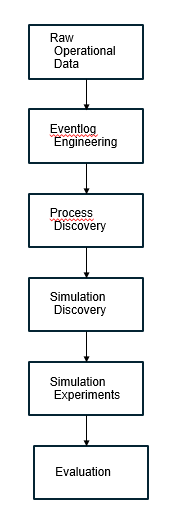
\includegraphics[width=0.95\textwidth]{figures/schemas/ResearchDesignV1.png}
\caption{Experimental pipeline. \emph{Data engineering} produces
\texttt{s6\_eventlog\_target\_rank\_features.csv} (Chapter~\ref{chp:case_study_and_data}).
The \emph{split} of Section~\ref{sec:train_test_split} separates the
log into training and held-out testing partitions. \emph{Process
discovery} (Section~\ref{sec:process_discovery_methodology}) yields the
Petri net used as the ProSiT skeleton. Three
\emph{simulation-parameter discovery} configurations
(Section~\ref{sec:simulation_discovery_methodology}) are compared;
each is evaluated against the held-out log through the
\emph{Monte-Carlo protocol} of Section~\ref{sec:mc_protocol}. Two
\emph{what-if} experiments (Section~\ref{sec:what_if_design}) exercise
the adopted-default configuration under operational disruption.}
\label{fig:research_design}
\end{figure}

%%%%%%%%%%%%%%%%%%%%%%%%%%%%%%%%%%%%%%%%%%%%%%%%%%%%%%%%%%%%%%%%%%%%%%%
\section{Research Questions, Hypotheses and Framing}
\label{sec:rq_h}
%%%%%%%%%%%%%%%%%%%%%%%%%%%%%%%%%%%%%%%%%%%%%%%%%%%%%%%%%%%%%%%%%%%%%%%

Chapter~\ref{chp:introduction} formulated the overarching research
questions. To make them empirically tractable, they are here refined
into testable claims. The claims deliberately admit rejection: an
outcome that contradicts a hypothesis is a valid contribution and is
reported as such in Chapter~\ref{chap:results}.

\subsection{Refined Research Questions}
\label{sec:refined_rq}

\begin{description}
\item[RQ1 (Fidelity).] To what extent does a ProSiT simulator
      discovered from historical CTB truck data reproduce case-level
      turnaround, activity durations, waiting times and arrivals on a
      held-out temporal test window?
\item[RQ2 (Structural quality).] Does the discovered Petri net
      generalise to the held-out period, or is fitness only preserved
      on the training period?
\item[RQ3 (Modelling choices).] How sensitive is simulation fidelity to
      three plausible ProSiT configurations
      (\textit{no-rules}, \textit{rules}, \textit{rules$+$workload})?
\item[RQ4 (Scenario support).] Does the discovered simulator produce
      operationally plausible KPI shifts under two transparent
      interventions: closing a single RMG block and increasing truck
      demand by 20\,\%?
\end{description}

\subsection{Hypotheses}
\label{sec:data_aware_hypotheses}

\begin{description}
\item[H1 (Time dependence of arrivals).] A time-aware arrival model
      (decision tree over hour, weekday, weekend indicator) reduces
      inter-arrival prediction error against a pooled-rate baseline on
      cross-validated hold-out slices from the training log.
\item[H2 (Data-aware fidelity gain).] Enabling ProSiT decision-tree
      rules (\textit{rules}) produces lower distributional distance to
      the held-out test log than the distribution-only ProSiT
      (\textit{no-rules}) for at least one of case-turnaround EMD,
      waiting-time EMD or service-time EMD.
\item[H3 (Workload-feature gain).] Adding queue-length and
      workload-history features to the ProSiT resource-selection and
      waiting-time models (\textit{rules$+$workload}) further reduces
      distributional distance versus \textit{rules} on the held-out
      test log.
\item[H4 (Scenario response).] Closing T22 eliminates assignments to
      that resource and increases RMG pre-service delay, while a
      20\,\% increase in working-time arrival intensity measurably
      increases the observed truck-arrival rate. Downstream
      turnaround effects are estimated rather than assumed.
\end{description}

Every hypothesis is intended to be falsifiable. In particular H2 and H3
are treated as claims of \emph{practical} benefit: the point estimate
must be lower and the 95\,\% confidence interval derived in
Section~\ref{sec:mc_protocol} must not overlap the reference configuration
entirely for the improvement to be reported as a fidelity gain.

%%%%%%%%%%%%%%%%%%%%%%%%%%%%%%%%%%%%%%%%%%%%%%%%%%%%%%%%%%%%%%%%%%%%%%%
\section{Held-Out Train/Test Split}
\label{sec:train_test_split}
%%%%%%%%%%%%%%%%%%%%%%%%%%%%%%%%%%%%%%%%%%%%%%%%%%%%%%%%%%%%%%%%%%%%%%%

\subsection{Rationale}

A held-out validation set is required to test H1--H3. In simulation
discovery it is not sufficient to report the fit of parameters on the
data used to discover them: a well-fit ProSiT bundle can memorise the
training distribution while over-fitting the operational dynamics. The
ProSiT reference implementation \cite{Vinci2026prosit} describes an
in-memory split in its \textit{Advanced Usage} example, but does not
persist the split, does not commit to a case-level boundary and does
not report validation metrics. This thesis therefore uses a persistent,
case-level, temporally ordered split that any downstream script can
consume unchanged.

\subsection{Split Definition}
\label{sec:split_definition}

Let $\mathcal{L}=(c_1,c_2,\dots,c_N)$ be the set of $N=89{,}460$ cases
in the final event log. For each case $c_i$ let $\tau(c_i)$ denote its
earliest event timestamp:
\begin{equation}
    \tau(c_i)=\min\bigl\{
      \text{start}(e),\text{time}(e)
      \mid e\in c_i \bigr\}.
\end{equation}
Sort the cases by $\tau$ and a deterministic case-identifier
tiebreaker. The first 80\,\% form the training set and the remaining
20\,\% form the test set. The cutoff $\tau^{\star}$ is recorded as the
earliest arrival in the test set. Cases whose earliest event timestamp
is missing are dropped from both.

On the CTB event log the cutoff is
$\tau^{\star}=\text{2026-04-20 18:17:00}$. The split produces 71,568
training cases (220,048 events) and 17,892 testing cases (55,360
events); no events are dropped. The split is realised by
\texttt{validation/01\_train\_test\_split.py} and is documented in
\texttt{validation/results/split\_manifest.json}, which also records
the seed, the cutoff and the per-activity coverage in both partitions.
The manifest is loaded by every downstream simulation script so that
$n_{\text{traces}}$ and $t_{\text{start}}$ match the test window
exactly.

\subsection{Correction Relative to Earlier Drafts}

Earlier versions of this thesis referenced a training set of 24,000
cases and a test set of 6,000 cases. Those numbers were an artefact of
a legacy random-subsample step in
\texttt{baseline/export\_empirical\_durations.py} that only fired when
the discovery scripts were pointed at the full event log. All discovery
scripts are now routed through
\texttt{baseline/\_eventlog\_source.py}, which prefers the persisted
\texttt{s6\_train.csv} and skips the legacy subsample when a train log
is detected. The correct partitioning is therefore 71,568/17,892 as
recorded in the split manifest.

%%%%%%%%%%%%%%%%%%%%%%%%%%%%%%%%%%%%%%%%%%%%%%%%%%%%%%%%%%%%%%%%%%%%%%%
\section{Process Discovery Protocol}
\label{sec:process_discovery_methodology}
%%%%%%%%%%%%%%%%%%%%%%%%%%%%%%%%%%%%%%%%%%%%%%%%%%%%%%%%%%%%%%%%%%%%%%%

\subsection{Algorithm}

The Petri net that ProSiT uses as the authoritative control-flow
skeleton is constructed from the observed training variants as a
sequential prefix trie. Every accepted path has the form
\texttt{Gate In}$\rightarrow$one or more yard activities
$\rightarrow$\texttt{Gate Out}. Shared prefixes are represented once,
and a separate transition encodes each observed continuation. This
prevents an inductive-miner concurrency cut from enabling two yard
activities inside the same truck visit. It does \emph{not} disable
multitasking between trucks: different cases still compete for and can
use resources concurrently according to the discovered capacities.

An inductive process tree is retained as a diagnostic visualisation,
but it is not passed to the final simulator. The authoritative trie is
implemented by \texttt{\_eventlog\_contract.py} and injected by
\texttt{baseline/07\_run\_prosit\_discovery.py}. It contains 76 places
and 144 transitions for the 70 variants observed in the frozen training
partition.

\subsection{Conformance Protocol}

Control-flow conformance metrics are computed against
\emph{both} the training and the held-out testing partition:

\begin{itemize}
    \item Token-based replay \textbf{fitness}, i.e.\ the fraction of
          traces that the Petri net can replay without token deficit.
    \item Token-based replay \textbf{precision}, the share of behaviour
          allowed by the model that is also observed in the log.
    \item \textbf{Generalisation} via
          \texttt{pm4py.generalization\_tbr}.
    \item \textbf{Simplicity} via \texttt{pm4py.simplicity\_petri\_net}.
\end{itemize}

They are supplemented by an explicit case-language audit: exactly one
initial Gate In, at least one yard activity, exactly one final Gate Out,
no within-case activity overlap and monotonically non-decreasing
completion timestamps. This separates two questions that aggregate
fitness alone cannot answer: whether the net replays held-out variants
and whether the generated traces obey the physical truck-visit order.
The full protocol is implemented in
\texttt{baseline/07\_run\_prosit\_discovery.py} and
\texttt{\_eventlog\_contract.py}.

%%%%%%%%%%%%%%%%%%%%%%%%%%%%%%%%%%%%%%%%%%%%%%%%%%%%%%%%%%%%%%%%%%%%%%%
\section{Simulation Parameter Discovery Configurations}
\label{sec:simulation_discovery_methodology}
%%%%%%%%%%%%%%%%%%%%%%%%%%%%%%%%%%%%%%%%%%%%%%%%%%%%%%%%%%%%%%%%%%%%%%%

ProSiT is used unchanged as the discovery and simulation engine
\cite{Vinci2026prosit}. All simulation parameters are learned by
\texttt{SimulatorParameters.discover\_from\_eventlog} from the training
partition only. Three configurations are evaluated. They are chosen so
that H2 (data-aware fidelity gain) and H3 (workload-feature gain) each
correspond to exactly one comparison.

\subsection{Configuration \textit{no-rules}}
\label{sec:cfg_no_rules}

The \textit{no-rules} configuration uses
\texttt{max\_depth\_tree}$=0$, which disables the ProSiT decision-tree
mechanism entirely. Every parameter reduces to a single unconditional
distribution or a marginal frequency: one arrival-rate distribution,
one execution-time distribution per activity, one waiting-time
distribution per resource, one categorical distribution over routing
choices at each Petri-net decision point. This configuration is the
distribution-based baseline against which H2 is tested.

\subsection{Configuration \textit{rules}}
\label{sec:cfg_rules}

The \textit{rules} configuration uses the ProSiT default
(\texttt{max\_depth\_tree}$=3$,
\texttt{min\_samples\_leaf\_cv}$=[50,100,200]$,
\texttt{random\_state}$=42$). Every timing, routing and
resource-selection model is fitted as a decision tree whose leaves
carry the local distributions. Cross-validation over the leaf-size grid
selects the actual leaf size per model, and models that fail to beat
the marginal distribution on held-out CRPS collapse to the pooled
baseline (this is a ProSiT internal safeguard against overfitting to
noise \cite{Vinci2026prosit}). Case-level attributes made available to
the trees are the container, demand, utilisation, target-area and
temporal features listed in
Section~\ref{sec:eventlog_structure}.

\subsection{Configuration \textit{rules$+$workload}}
\label{sec:cfg_workload}

The \textit{rules$+$workload} configuration is identical to
\textit{rules} but with
\texttt{use\_workload\_features}$=$\texttt{True}. As documented in the
ProSiT README this enables two extra features on the waiting-time and
resource-selection models: current workload (number of concurrent
tasks) and queue length (number of tasks scheduled but not yet started)
at the time each event is enabled in the process model. The intention behind including this
configuration is to let ProSiT see the queueing state that its
distribution family alone would otherwise ignore. This configuration is
compared against \textit{rules} to test H3.

\subsection{Discovery Hyperparameters}

Table~\ref{tab:prosit_hyperparams} lists the ProSiT hyperparameters
that differ across configurations. All other arguments are the ProSiT
defaults except \texttt{attribute\_mode}, which is set to
\texttt{'empirical'} for reasons detailed in
Section~\ref{sec:prosit_workarounds}.

\begin{table}[h]
\centering
\caption{ProSiT discovery hyperparameters by configuration.}
\label{tab:prosit_hyperparams}
\begin{tabular}{lccc}
\toprule
\textbf{Hyperparameter} & \textbf{no-rules} & \textbf{rules} & \textbf{rules$+$workload} \\
\midrule
\texttt{max\_depth\_tree}          & 0             & 3             & 3 \\
\texttt{min\_samples\_leaf\_cv}    & --            & [50, 100, 200] & [50, 100, 200] \\
\texttt{use\_workload\_features}   & False         & False         & True \\
\texttt{attribute\_mode}           & \texttt{empirical} & \texttt{empirical} & \texttt{empirical} \\
\texttt{random\_state}             & 42            & 42            & 42 \\
\bottomrule
\end{tabular}
\end{table}

The full pipeline is executed by
\texttt{baseline/07\_run\_prosit\_discovery.py}. The pickled
\texttt{SimulatorParameters} objects
(\texttt{prosit\_params.pkl}) and their JSON representations are stored
in the paramset folder
\path{baseline/discovery_params/params_<utc>_train80/prosit_discovery_no_rules|_workload|/}.

%%%%%%%%%%%%%%%%%%%%%%%%%%%%%%%%%%%%%%%%%%%%%%%%%%%%%%%%%%%%%%%%%%%%%%%
\section{Monte-Carlo Replication Protocol}
\label{sec:mc_protocol}
%%%%%%%%%%%%%%%%%%%%%%%%%%%%%%%%%%%%%%%%%%%%%%%%%%%%%%%%%%%%%%%%%%%%%%%

Every ProSiT simulation includes stochastic draws from the fitted
distributions. Reporting a single Monte-Carlo draw is therefore
insufficient to conclude that one configuration is more faithful than
another: the observed difference may be within the sampling variance
of the simulator itself. This thesis therefore reports every fidelity
metric with a Monte-Carlo confidence interval.

\subsection{Replication Design}

For each ProSiT configuration
$\text{cfg}\in\{\textit{no-rules},\textit{rules},\textit{rules$+$workload}\}$
the following procedure is executed:

\begin{enumerate}
    \item Load the corresponding \texttt{SimulatorParameters} bundle
          from disk.
    \item Instantiate a fresh \texttt{SimulatorEngine}.
    \item For $i=0,\dots,N_{\text{seeds}}-1$:
          \begin{enumerate}
              \item Seed Python's \texttt{random} and
                    \texttt{numpy.random} with $\text{base}+i$.
              \item Simulate $n_{\text{traces}}=17{,}892$ cases starting
                    at
                    $t_{\text{start}}=\text{2026-04-20 18:17:00}$, i.e.\
                    the test-window cutoff read from
                    \texttt{split\_manifest.json}.
              \item Compute the fidelity metrics of
                    Section~\ref{sec:evaluation_metrics} against the
                    held-out test log.
          \end{enumerate}
    \item Aggregate the $N_{\text{seeds}}$ replications into a Student-t
          95\,\% confidence interval per metric:
          $\bar x \pm t_{0.975,\,N-1}\, s/\sqrt{N}$.
\end{enumerate}

\subsection{Implementation}

The protocol is implemented in
\texttt{validation/06\_multi\_seed\_ci.py}. \(N_{\text{seeds}}=10\) is
used for every configuration, following the sample-size heuristic that
a Student-t interval on four KPIs is meaningful at $N=10$ while
remaining computationally affordable at $\sim$50\,seconds per
simulation. The base seed is 42.

The choice to seed Python's \texttt{random} and \texttt{numpy.random}
before each \texttt{engine.apply()} rather than the ProSiT engine
itself is intentional: ProSiT 1.0.3 does not expose a per-call seed on
its simulation engine. Seeding both random-number generators before the
call yields reproducible replications and captures the same stochastic
variability that a user would observe in production.

%%%%%%%%%%%%%%%%%%%%%%%%%%%%%%%%%%%%%%%%%%%%%%%%%%%%%%%%%%%%%%%%%%%%%%%
\section{Fidelity Metrics}
\label{sec:evaluation_metrics}
%%%%%%%%%%%%%%%%%%%%%%%%%%%%%%%%%%%%%%%%%%%%%%%%%%%%%%%%%%%%%%%%%%%%%%%

The comparison of a simulated event log against the real held-out log
uses four distributional distance metrics. Each metric is computed once
per Monte-Carlo replication so that a confidence interval can be
attached to the point estimate.

\subsection{Wasserstein Distance (EMD)}

For each activity $a$ the service-time EMD is
\begin{equation}
    \text{EMD}_a^{\text{svc}} = W_1
    \bigl(F_{a}^{\text{sim,svc}}, F_{a}^{\text{real,svc}}\bigr),
\end{equation}
where $F_{a}^{\text{sim,svc}}$ and $F_{a}^{\text{real,svc}}$ are the
empirical CDFs of $\text{time}-\text{start}$ for activity $a$ in the
simulated and real log, respectively. The pre-service-delay EMD is defined
analogously on $\text{start}-\text{enabled}_{\text{model}}$ using the
model-derived enablement timestamps from ProSiT's simulated log. The per-activity means
are the ``mean service-time EMD'' and ``mean waiting-time EMD''
reported in Chapter~\ref{chap:results}. The case-level turnaround EMD
is $W_1(F^{\text{sim,ttot}}, F^{\text{real,ttot}})$ where
$\text{ttot}$ is the total elapsed time per case (first start to last
complete). The inter-arrival EMD is
$W_1(F^{\text{sim,iat}}, F^{\text{real,iat}})$ where
$\text{iat}$ is the time between consecutive case-arrival timestamps.
All EMDs are reported in minutes.

\subsection{Kolmogorov--Smirnov Statistic}

For each distribution pair the two-sample KS statistic is computed by
\texttt{scipy.stats.ks\_2samp}. Because the CTB test log contains 55,360
events, sub-sampling is applied so that each side contributes at most
$10{,}000$ observations to the test. This keeps the $p$-value
informative and prevents the null from being rejected mechanically by
sample size. The KS statistic (magnitude of the maximum vertical CDF
gap) is reported alongside the EMD; the $p$-value is retained for the
appendix.

\subsection{Point-Statistic Errors}

For each activity and each case-level KPI the mean, median and 90th
percentile of the simulated and real distributions are compared as
absolute and relative errors. This complements the distributional
metrics with operationally interpretable point statistics
(e.g.\ ``the simulator under-predicts mean turnaround by $X$ minutes'').

\subsection{Implementation}

The metric definitions are implemented in
\texttt{validation/02\_validate\_simulation.py} and reused verbatim by
\texttt{validation/06\_multi\_seed\_ci.py} to guarantee that
single-shot and multi-seed numbers are directly comparable.

%%%%%%%%%%%%%%%%%%%%%%%%%%%%%%%%%%%%%%%%%%%%%%%%%%%%%%%%%%%%%%%%%%%%%%%
\section{What-If Scenario Design}
\label{sec:what_if_design}
%%%%%%%%%%%%%%%%%%%%%%%%%%%%%%%%%%%%%%%%%%%%%%%%%%%%%%%%%%%%%%%%%%%%%%%

Two independent interventions are evaluated to test H4. Both are
derived by deep copy from the frozen, training-only calibrated
\textit{rules$+$workload} baseline. No held-out observation is used to
select or fit a scenario parameter.

\subsection{Scenario A: T22 Closure}

Scenario A models a full closure of RMG block T22. The scenario is
constructed by (i) removing T22 from every
\texttt{params.act\_to\_resources} entry that references it, after
verifying that each affected activity retains at least one eligible
resource; and (ii) setting all 168 weekly calendar slots of T22 to
unavailable. All other parameters are unchanged.

This is a capacity-eligibility intervention, not a spatial yard model.
The discovered selector may use target-area attributes as statistical
predictors, but ProSiT does not impose a hard constraint that binds a
container to its actually observed storage block. A truck whose
historical target was T22 can therefore be assigned to another eligible
block without an explicit container-relocation operation or a
location-dependent travel-time adjustment. This boundary is evaluated
explicitly in Section~\ref{sec:limitations}.

\subsection{Scenario B: 20\,\% Higher Truck Demand}

Scenario B changes only the empirical working-time inter-arrival
distribution. For demand multiplier $m=1.20$, every empirical
inter-arrival sample $x_i$ is replaced by $x_i/m$. This preserves the
zero mass and the empirical distribution shape while increasing the
modelled arrival intensity by exactly 20\,\%. The gate-admission
calendar, process model, duration models, routing, resource mappings,
resource calendars and case-attribute schema remain unchanged. The
scenario is independent of the T22 closure.

\subsection{Domain-Constrained RMG Capacity Sensitivity}

The serialized baseline assigns maximum concurrency four to ten RMG
block identifiers and five to twelve, for an aggregate effective upper
bound of 100. This exceeds the operational limit of at most three cranes
per block. A separate sensitivity baseline is therefore derived by
replacing every RMG value $c_r$ with
$\min(c_r,3)$. The aggregate bound becomes $22\times3=66$. No resource
mapping, calendar, selection rule, timing model, arrival model or
control-flow parameter is changed. The T22 and demand interventions are
then independently re-derived from this capped baseline.

This is a robustness test rather than a recalibration: the discovered
baseline remains frozen and authoritative. It asks whether conclusions
conditional on effective capacity 100 persist under the stated physical
upper bound. Both sets of replications use identical seeds, trace counts
and start time. In addition to direct cap effects, the analysis reports
the interaction
\begin{equation}
\Delta_{\mathrm{interaction}}=
(Y_{\mathrm{scenario}}-Y_{\mathrm{baseline}})_{c\leq3}
-(Y_{\mathrm{scenario}}-Y_{\mathrm{baseline}})_{\mathrm{discovered}},
\end{equation}
so that changes in scenario response are not confused with a general
level shift caused by the cap.

\subsection{Reporting}

The unified driver \texttt{validation/09\_multi\_seed\_scenarios.py}
executes baseline and both interventions with ten matched seeds
(42--51), $n_{\text{traces}}=17{,}892$ and
$t_{\text{start}}=\text{2026-04-20 18:17}$. Thus all paired deltas use
common random numbers. Mean, median and 90th percentile of turnaround,
RMG service and RMG pre-service delay are reported together with the
observed arrival KPIs. Every one of the 30 generated logs is subjected
to the sequential case contract of
Section~\ref{sec:process_discovery_methodology}; any violation aborts
the run. The same driver executes the additional 30 capped replications.
\texttt{validation/10\_compare\_rmg\_capacity\_sensitivity.py} verifies
identical source hashes and settings before computing the paired direct
effects and interactions. Thus 60 scenario logs are audited in total.

%%%%%%%%%%%%%%%%%%%%%%%%%%%%%%%%%%%%%%%%%%%%%%%%%%%%%%%%%%%%%%%%%%%%%%%
\section{Descriptive Transition-Duration Analysis}
\label{sec:results_percentile_sens_design}
%%%%%%%%%%%%%%%%%%%%%%%%%%%%%%%%%%%%%%%%%%%%%%%%%%%%%%%%%%%%%%%%%%%%%%%

As discussed in Section~\ref{sec:abandoned_baseline}, an earlier
pipeline version reconstructed activity enablement from route-specific
transition baselines. Although this approach was abandoned in favour of
ProSiT's internal model-derived enablement, the empirical transition
durations remain informative as descriptive evidence of the physical
separation between terminal activities.

To characterise this physical component, the same baseline table is
recomputed with the 5th, 10th, 25th and 50th percentiles as
alternative choices. For each transition $(a,b)$ with at least twenty
observations the resulting baseline duration is reported together with
the shift relative to the 5th percentile and the rank correlation
between percentiles. This analysis is implemented in
\texttt{validation/04\_baseline\_percentile\_sensitivity.py} and
reported in Section~\ref{sec:results_percentile_sens}. It does
\textbf{not} affect ProSiT's simulation-parameter discovery; its
purpose is to illustrate that the model-derived pre-service delay
includes a non-trivial physical-movement component that cannot be
separated from operational waiting with the available data.

%%%%%%%%%%%%%%%%%%%%%%%%%%%%%%%%%%%%%%%%%%%%%%%%%%%%%%%%%%%%%%%%%%%%%%%
\section{ProSiT Implementation Notes and Workarounds}
\label{sec:prosit_workarounds}
%%%%%%%%%%%%%%%%%%%%%%%%%%%%%%%%%%%%%%%%%%%%%%%%%%%%%%%%%%%%%%%%%%%%%%%

Applying ProSiT 1.0.3 \cite{Vinci2026prosit} to the CTB event log
uncovered several implementation issues that would have propagated as
silent misbehaviour if not addressed. This section documents them so
that the experiments can be reproduced deterministically and so that the
downstream fidelity numbers can be interpreted correctly.

\subsection{Data-Attribute Discovery on NaN Columns}

The default \texttt{attribute\_mode='distribution'} passes each case
attribute through a per-attribute distribution fitter. In the CTB log,
\texttt{full\_ratio} and \texttt{is\_full} contain \texttt{NaN} for
cases that involve empty-container-only visits. The distribution fitter
in ProSiT 1.0.3 forwards the raw values to
\texttt{scipy.stats}, which raises
\texttt{TypeError: ufunc 'isfinite' not supported} on the mixed
dtype. Switching to \texttt{attribute\_mode='empirical'} bypasses the
per-attribute fitter and samples full attribute tuples from the
observed joint distribution instead. This is not a fidelity compromise:
the discovered simulator still preserves case-level attribute
correlations, and empirical sampling from the training distribution is
the appropriate choice given the number of categorical attributes
present in the CTB log.

\subsection{Simulation in No-Rules Mode}

In \textit{no-rules} mode ProSiT samples the routing choice via
\texttt{random.choice(seq)} where \texttt{seq} is a
\texttt{numpy.ndarray}. Python's built-in \texttt{random.choice}
evaluates \texttt{if not seq:}, which raises
\texttt{ValueError: The truth value of an array with more than one
element is ambiguous.} on multi-element numpy arrays. The workaround is
a minimal monkey patch that intercepts \texttt{random.choice} while the
engine is running and forwards \texttt{numpy.ndarray} arguments through
\texttt{numpy.random.randint}. The patch is contained to the
simulation call and is restored immediately afterwards. It is applied
by both \texttt{baseline/07\_run\_prosit\_discovery.py} and
\texttt{validation/06\_multi\_seed\_ci.py}.

\subsection{Duplicated Columns in the Simulated Log}

ProSiT 1.0.3 writes case-level attributes into the event-level frame
returned by \texttt{SimulatorEngine.apply()}. When a case-level
attribute has the same name as an event attribute (in the CTB log this
happens for \texttt{enabled:timestamp} because ProSiT writes case-level
attributes into the event-level frame), the resulting
\texttt{pandas.DataFrame}
carries duplicate column labels. Standard operations such as
\texttt{pd.to\_datetime(df[col])} then return a \texttt{DataFrame} slice
instead of a \texttt{Series} and fail. The workaround is a single
\texttt{df.loc[:, \textasciitilde df.columns.duplicated()]} call at the
start of every KPI-computation function. It is applied both in the
what-if scripts and in the multi-seed CI driver.

\subsection{Absence of Automatic Temporal Features}

ProSiT does not derive hour-of-day or day-of-week features from the
event-log timestamps during simulation-parameter discovery: temporal
features must be provided as explicit case attributes. This is why the
event-log engineering pipeline of
Section~\ref{sec:temporal_features} adds
\texttt{@@hour} and \texttt{@@weekday} at case level. Without them,
ProSiT's arrival-time and duration models cannot condition on the
strong day/night pattern that Section~\ref{sec:results_arrival_process}
documents.

\subsection{Non-Deterministic Simulation Engine}

\texttt{SimulatorEngine.apply()} does not accept an explicit seed. The
Monte-Carlo protocol of Section~\ref{sec:mc_protocol} therefore seeds
Python's \texttt{random} and \texttt{numpy.random} before every call to
\texttt{apply()}. Two consecutive calls with different seeds produce
different logs; two consecutive calls with the same seed produce the
same log up to floating-point noise. This is the reproducibility
guarantee assumed throughout Chapter~\ref{chap:results}.

\subsection{Contribution Boundary}

The ProSiT engine itself was not modified for these workarounds. The
CTB pipeline patches its own callers so that ProSiT can be invoked
without source-code changes. All five workarounds together constitute
the technical adaptation of ProSiT to the CTB case study and are
listed here so that a reader can distinguish the contribution of this
thesis (case-study specific data engineering, held-out validation
methodology, multi-seed replication, sensitivity analysis, what-if
scenario protocol) from the contribution of ProSiT itself
(automatic simulation-parameter discovery from event logs
\cite{Vinci2026prosit}).


    \chapter{Results}
\label{chap:results}

This chapter reports the empirical evidence produced by the pipeline
defined in Chapter~\ref{chp:experiments_and_framework}. Every number in
this chapter is traceable to a script and an artefact in the
repository; every claim is qualified by its confidence interval or its
inherent uncertainty. The chapter is organised so that the reader
encounters the evidence in the same order in which the hypotheses of
Section~\ref{sec:data_aware_hypotheses} depend on it.

Section~\ref{sec:results_eventlog_char} reports the descriptive
characteristics of the training and testing partitions produced by the
split of Section~\ref{sec:train_test_split}.
Section~\ref{sec:results_process_discovery} reports the discovered
Petri net and its conformance on both partitions (RQ2).
Section~\ref{sec:results_arrival_process} reports the temporal
structure of the arrival process (H1).
Section~\ref{sec:results_holdout_fidelity} reports the held-out
Monte-Carlo fidelity of the three ProSiT configurations
(RQ1, H2, H3). Section~\ref{sec:results_per_activity} decomposes the
fidelity by activity to identify where each configuration wins or
loses. Section~\ref{sec:results_resource_capacities} reports the
discovered resource capacities and their limits.
Section~\ref{sec:results_percentile_sens} reports the sensitivity of
the transition-baseline choice (RQ3).
Section~\ref{sec:results_scenarios} reports the two what-if scenarios
(H4). Section~\ref{sec:results_summary} consolidates the empirical
findings against the hypotheses.

%%%%%%%%%%%%%%%%%%%%%%%%%%%%%%%%%%%%%%%%%%%%%%%%%%%%%%%%%%%%%%
\section{Event Log Characteristics on the Held-Out Split}
\label{sec:results_eventlog_char}
%%%%%%%%%%%%%%%%%%%%%%%%%%%%%%%%%%%%%%%%%%%%%%%%%%%%%%%%%%%%%%

The train/test split of Section~\ref{sec:train_test_split} yields a
temporally ordered partition of the 89,458 cases. Cases with earliest
event timestamp $\le\text{2026-04-20 18:14}$ form the training log
(71,566 cases, 221,559 events, cases spanning
\text{2026-03-02 05:25} through the cutoff). Cases with earliest event
timestamp $>\text{2026-04-20 18:14}$ form the testing log (17,892
cases, 55,864 events). No events are dropped for missing timestamps.
Table~\ref{tab:activity_counts_split} lists the per-activity counts in
both partitions.

\begin{table}[h]
\centering
\caption{Activity counts on the train and test partitions.}
\label{tab:activity_counts_split}
\begin{tabular}{lrrr}
\toprule
\textbf{Activity} & \textbf{Train} & \textbf{Test} & \textbf{Total} \\
\midrule
Gate In       & 71,566 & 17,892 & 89,458 \\
Gate Out      & 71,566 & 17,892 & 89,458 \\
RMG\_receive  & 30,656 & 7,678  & 38,334 \\
RMG\_delivery & 14,010 & 3,514  & 17,524 \\
RMG\_mixed    & 10,816 & 2,706  & 13,522 \\
LL\_delivery  & 7,678  & 1,911  & 9,589  \\
HO2\_delivery & 5,351  & 1,338  & 6,689  \\
HO2\_receive  & 3,807  & 955    & 4,762  \\
LL\_mixed     & 3,571  & 880    & 4,451  \\
HO2\_mixed    & 1,810  & 444    & 2,254  \\
LL\_receive   & 728    & 182    & 910    \\
\bottomrule
\end{tabular}
\end{table}

The per-activity distribution on the test partition is proportional to
the training partition to within 1--3\,\% for the four RMG-related
activities and within 5\,\% for the low-frequency activities
(\texttt{LL\_receive}, \texttt{HO2\_mixed}). No activity is missing from
the test partition. The split therefore does not introduce
class-imbalance artefacts that would confound the fidelity comparison
in Section~\ref{sec:results_holdout_fidelity}.

%%%%%%%%%%%%%%%%%%%%%%%%%%%%%%%%%%%%%%%%%%%%%%%%%%%%%%%%%%%%%%
\section{Process Discovery and Held-Out Conformance}
\label{sec:results_process_discovery}
%%%%%%%%%%%%%%%%%%%%%%%%%%%%%%%%%%%%%%%%%%%%%%%%%%%%%%%%%%%%%%

The Petri net is discovered from the training partition with the
inductive miner as described in
Section~\ref{sec:process_discovery_methodology}. Table~\ref{tab:conformance_train_test}
reports the four conformance metrics on both partitions.

\begin{table}[h]
\centering
\caption{Petri-net conformance on train and test.}
\label{tab:conformance_train_test}
\begin{tabular}{lrr}
\toprule
\textbf{Metric} & \textbf{Train} & \textbf{Test} \\
\midrule
Fitness (token-based replay)     & 1.000 & 1.000 \\
Precision (token-based replay)   & 0.904 & 0.872 \\
Generalisation                   & 0.974 & 0.949 \\
Simplicity                       & 0.652 & 0.652 \\
\bottomrule
\end{tabular}
\end{table}

Fitness of $1.000$ on the training log is expected: the inductive miner
is fitness-preserving by construction. Fitness of $1.000$ on the
held-out testing log is not automatic: it demonstrates that the
control-flow structure discovered on the first 80\,\% of the cases
replays every case in the last 20\,\% without token deficit. Precision
drops from 0.904 to 0.872 (a relative reduction of 3.5\,\%) and
generalisation from 0.974 to 0.949 (a relative reduction of 2.6\,\%).
Simplicity depends only on the Petri-net structure and is identical
across partitions.

The size of the discovered Petri net is 42 places, 59 transitions and
128 arcs. The training log contains 134 trace variants; the top-3
variants account for 67.5\,\% of all cases and the top-20 variants for
98.7\,\%. The remaining variants correspond to low-frequency
operational deviations
(e.g.\ \texttt{Gate In}$\to$\texttt{HO2\_mixed}$\to$\texttt{LL\_delivery}$\to$\texttt{Gate Out}
with 41 cases).

Figure~\ref{fig:petri_net} shows the discovered Petri net enriched with
token-replay frequency; edge labels report the number of tokens that
crossed the corresponding transition during replay on the training log.
The visualisation makes the process structure explicit: after
\texttt{Gate In} the flow branches at a first exclusive choice
between RMG, LL and HO2 handling; the three handling families each
carry an internal exclusive choice between \texttt{receive},
\texttt{delivery} and \texttt{mixed} sub-activities; the flow
re-converges before \texttt{Gate Out}. The relative arc thickness
mirrors the activity counts of Table~\ref{tab:activity_counts_split}:
the RMG family dominates ($\approx 63\,\%$ of yard activities), the LL
family follows ($\approx 21\,\%$) and the HO2 family is the least
frequent ($\approx 16\,\%$). No unreachable transitions or dead places
appear in the net.

\begin{figure}[htbp]
\centering
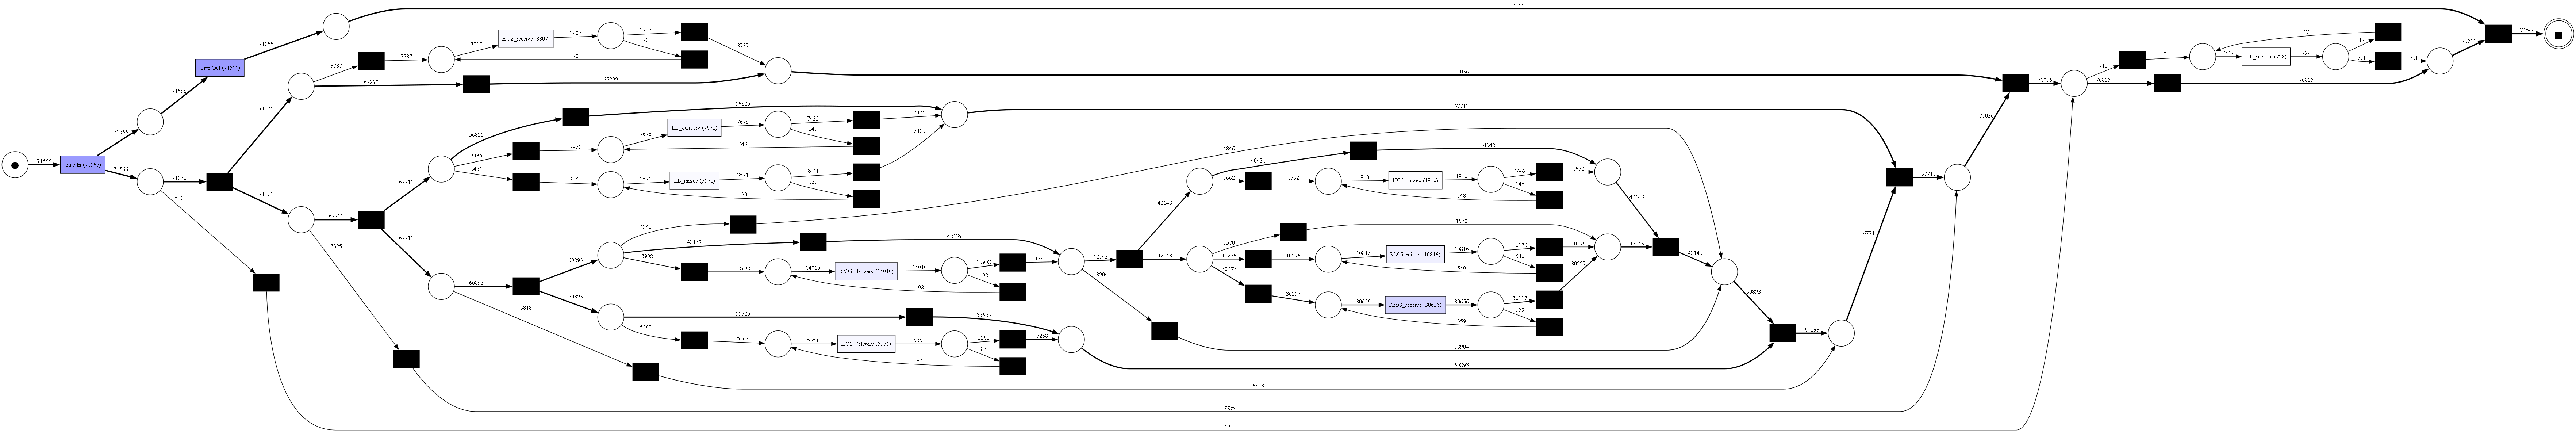
\includegraphics[width=0.95\textwidth]{figures/discovery/petri_net_frequency.png}
\caption{Discovered Petri net with token-replay frequency on the
training log (71,566 cases, 221,559 events). Transition labels report
the number of replayed tokens. The visualisation is produced by
\texttt{pm4py.visualization.petri\_net.visualizer} in the
\texttt{FREQUENCY} variant.}
\label{fig:petri_net}
\end{figure}

Figure~\ref{fig:dfg_freq} shows the directly-follows graph of the
training log. This is a complementary view to the Petri net:
whereas the Petri net encodes the concurrency and exclusive choice
structure inferred by the inductive miner, the DFG shows the raw
handover statistics between activities. The dominant paths
\texttt{Gate~In}$\to$\texttt{RMG\_receive}$\to$\texttt{Gate~Out},
\texttt{Gate~In}$\to$\texttt{RMG\_delivery}$\to$\texttt{Gate~Out} and
\texttt{Gate~In}$\to$\texttt{RMG\_mixed}$\to$\texttt{Gate~Out}
carry 30k, 14k and 11k cases respectively.

\begin{figure}[htbp]
\centering
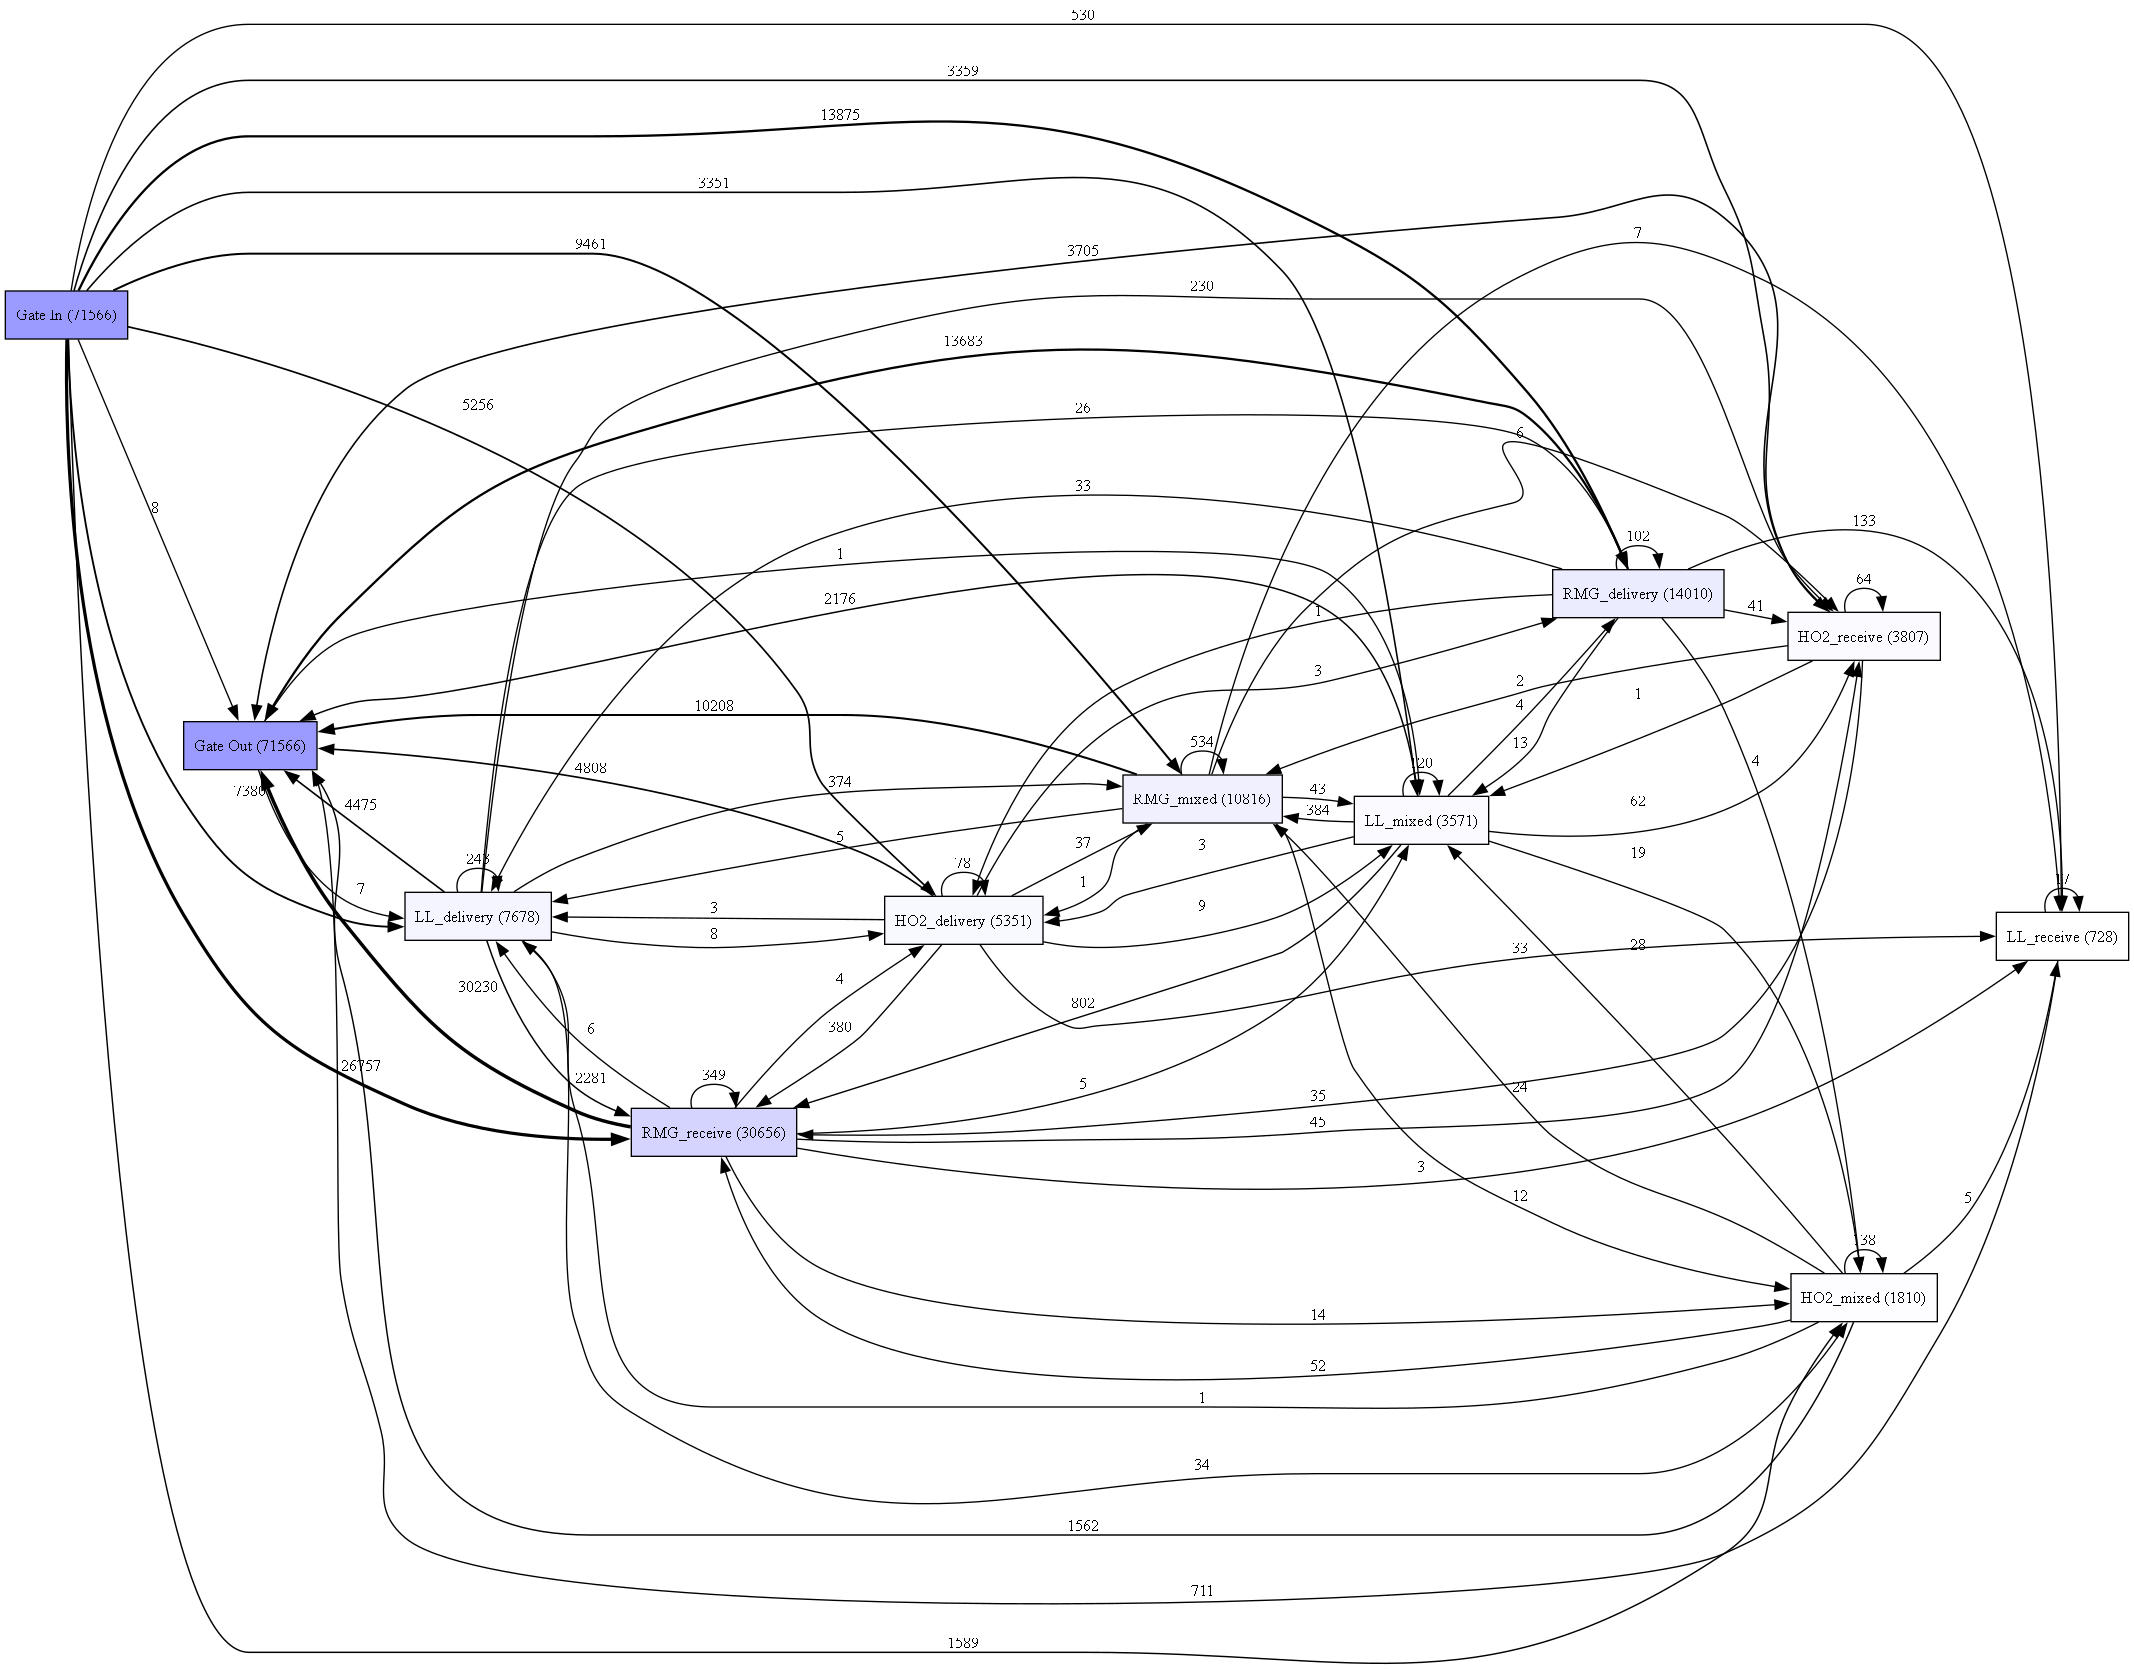
\includegraphics[width=0.85\textwidth]{figures/discovery/dfg_frequency.png}
\caption{Directly-follows graph of the training log with edge
frequencies. Complementary to the Petri net in
Figure~\ref{fig:petri_net}: shows raw handover statistics between
activities.}
\label{fig:dfg_freq}
\end{figure}

Figure~\ref{fig:variants_top20} confirms the concentration of behaviour
in a small number of variants. The top 20 trace variants cover 98.7\,\%
of the 71,566 training cases; the tail of 114 additional variants
accounts for only 908 cases and consists mainly of visits that combine
two yard families in a single visit (e.g.\ HO2 receive followed by an
RMG delivery). The event log is therefore structurally regular: the
Petri net of Figure~\ref{fig:petri_net} is a compact representation of
the observed control flow, not a coarse simplification of a highly
variable process.

\begin{figure}[htbp]
\centering
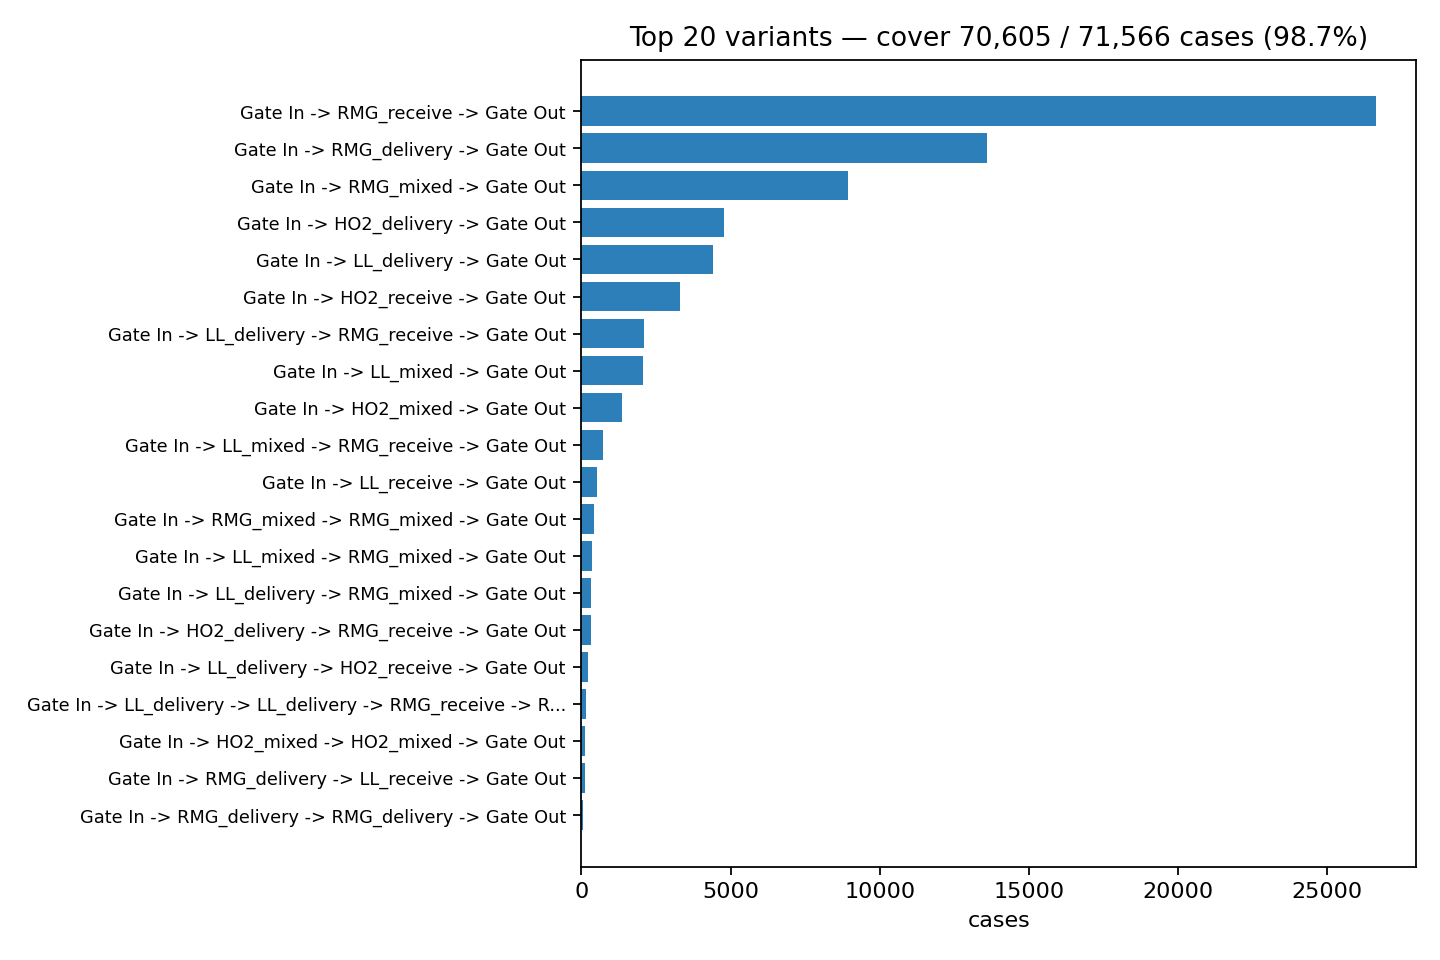
\includegraphics[width=0.9\textwidth]{figures/discovery/variants_top20.png}
\caption{Trace-variant coverage on the training log. The top 20 of the
134 observed variants cover 98.7\,\% of the 71,566 cases; the label
next to each variant reports the number of cases following it.}
\label{fig:variants_top20}
\end{figure}

\medskip

\noindent\textbf{RQ2 (structural quality).} The control-flow model
generalises to the held-out period: fitness stays at $1.0$ and the
precision and generalisation reductions are modest. The Petri net is
therefore a legitimate skeleton for the simulation-parameter discovery
that follows.

%%%%%%%%%%%%%%%%%%%%%%%%%%%%%%%%%%%%%%%%%%%%%%%%%%%%%%%%%%%%%%
\section{Temporal Structure of the Arrival Process}
\label{sec:results_arrival_process}
%%%%%%%%%%%%%%%%%%%%%%%%%%%%%%%%%%%%%%%%%%%%%%%%%%%%%%%%%%%%%%

The arrival process is the clearest case for time-conditioning in the
CTB event log. Table~\ref{tab:arrival_benchmark} compares a pooled
arrival-rate baseline (a single global mean) against a time-aware
decision tree (features: hour, weekday, weekend indicator) on 30-minute
arrival counts derived from the training partition. Both models are
evaluated on a chronological 80/20 split within the training partition
so that the numbers reflect the same temporal-hold-out logic used for
the simulator evaluation later.

\begin{table}[h]
\centering
\caption{Arrival-rate benchmark on 30-minute buckets (training log only,
chronological 80/20 split).}
\label{tab:arrival_benchmark}
\begin{tabular}{lrrr}
\toprule
\textbf{Model} & \textbf{MAE} & \textbf{RMSE} & \textbf{$R^{2}$} \\
\midrule
Pooled arrival rate         & 28.98 & 34.60 & $-0.001$ \\
Time-aware decision tree    & \textbf{9.41}  & \textbf{16.87} & \textbf{0.762} \\
\bottomrule
\end{tabular}
\end{table}

The pooled baseline has an $R^{2}$ indistinguishable from zero: a
single global arrival rate has no predictive power for 30-minute
arrival counts on this dataset. The time-aware tree reduces MAE by
67.5\,\% and RMSE by 51.2\,\% and achieves $R^{2}=0.762$. The day/night
statistics of Table~\ref{tab:day_night} confirm the underlying
non-stationarity: mean arrivals per hour rise from 12.8 at night to
110.9 during the day, an $8.7\times$ difference that a pooled model
cannot represent.

\begin{table}[h]
\centering
\caption{Day vs.\ night arrival statistics on the training log.}
\label{tab:day_night}
\begin{tabular}{lrrr}
\toprule
\textbf{Period} & \textbf{Mean inter-arrival (min)} & \textbf{Mean arrivals/hour} & \textbf{Cases} \\
\midrule
All   & 1.00  & 60.2   & 71,566 \\
Day   & 0.54  & 110.9  & 63,710 \\
Night & 4.69  & 12.8   & 7,856  \\
\bottomrule
\end{tabular}
\end{table}

\medskip

\noindent\textbf{H1 (time dependence of arrivals) is accepted.} The
time-aware arrival model reduces MAE by 67.5\,\% and RMSE by 51.2\,\%
relative to a pooled baseline on a chronological within-training
hold-out. This is a substantial and interpretable effect. The
day/night contrast (Table~\ref{tab:day_night}) is the operational
mechanism that the tree captures.

%%%%%%%%%%%%%%%%%%%%%%%%%%%%%%%%%%%%%%%%%%%%%%%%%%%%%%%%%%%%%%
\section{Held-Out Simulation Fidelity (Multi-Seed)}
\label{sec:results_holdout_fidelity}
%%%%%%%%%%%%%%%%%%%%%%%%%%%%%%%%%%%%%%%%%%%%%%%%%%%%%%%%%%%%%%

The three ProSiT configurations of
Section~\ref{sec:simulation_discovery_methodology} are evaluated
against the held-out test log using the Monte-Carlo protocol of
Section~\ref{sec:mc_protocol}. Each configuration is simulated with
$N_{\text{seeds}}=10$ independent seeds; every simulation covers
$n_{\text{traces}}=17{,}892$ cases starting at the test-window cutoff
$t_{\text{start}}=\text{2026-04-20 18:14}$. Table~\ref{tab:headline_ci}
reports the four headline fidelity metrics with 95\,\% Student-t
confidence intervals.

\begin{table}[h]
\centering
\caption{Held-out fidelity by ProSiT configuration
($N_{\text{seeds}}=10$; 95\,\% Student-t CI).}
\label{tab:headline_ci}
\begin{tabular}{lccc}
\toprule
\textbf{Metric (min)} &
\textbf{no-rules} &
\textbf{rules} &
\textbf{rules$+$workload} \\
\midrule
Service EMD (mean over activities) &
$1.89\;[1.81, 1.97]$ &
$1.98\;[1.88, 2.08]$ &
$1.98\;[1.92, 2.04]$ \\
Waiting EMD (mean over activities) &
$32.84\;[31.66, 34.02]$ &
$35.30\;[32.99, 37.61]$ &
$35.88\;[34.42, 37.35]$ \\
Case turnaround EMD &
$\mathbf{10.02\;[9.20, 10.85]}$ &
$11.25\;[9.88, 12.61]$ &
$11.62\;[10.77, 12.48]$ \\
Inter-arrival EMD &
$0.318\;[0.316, 0.319]$ &
$0.314\;[0.313, 0.316]$ &
$0.314\;[0.313, 0.316]$ \\
Case turnaround KS &
$0.070\;[0.066, 0.075]$ &
$0.072\;[0.067, 0.078]$ &
$0.073\;[0.067, 0.079]$ \\
\bottomrule
\end{tabular}
\end{table}

Figure~\ref{fig:three_way_ci} presents the same four EMD metrics as
point estimates with their 95\,\% confidence intervals so that the
pairwise overlaps are visually apparent.

\begin{figure}[htbp]
\centering
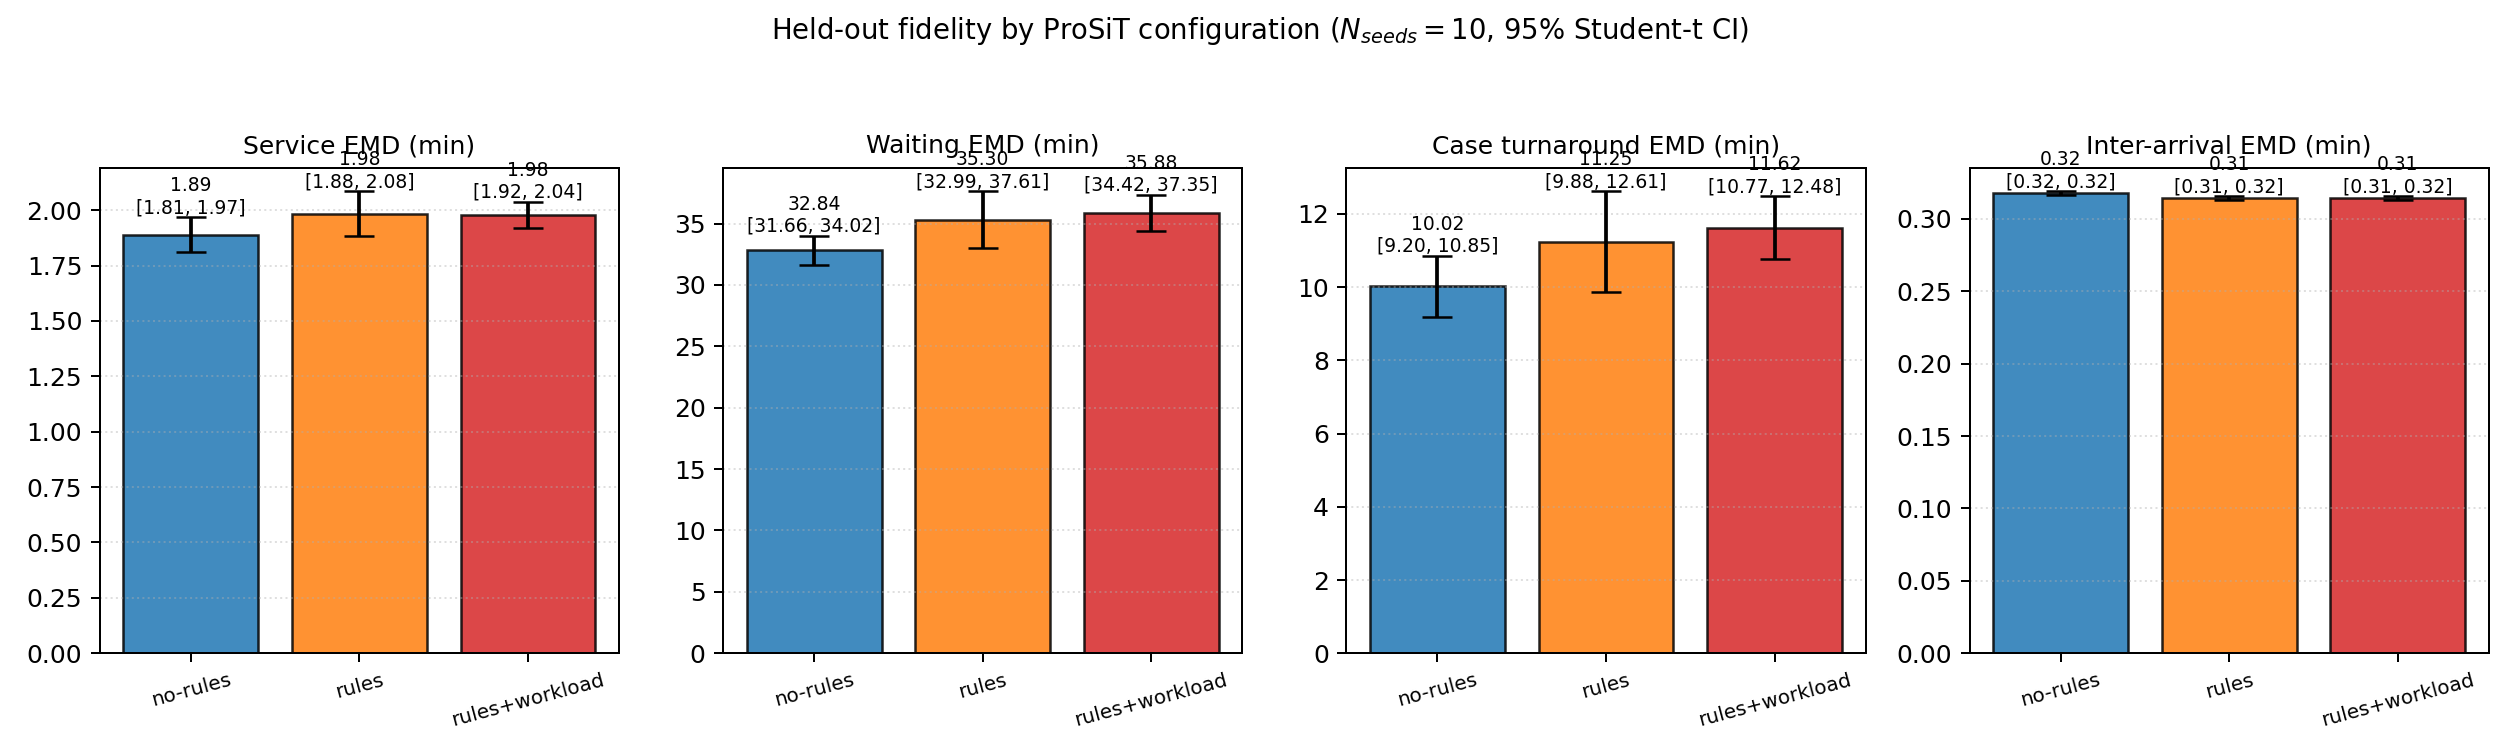
\includegraphics[width=\textwidth]{figures/three_way_ci.png}
\caption{Held-out fidelity by ProSiT configuration
($N_{\text{seeds}}=10$; 95\,\% Student-$t$ CI). Blue: no-rules
(distribution-only), orange: rules (data-aware trees), red:
rules$+$workload (trees with queue-length features). Numbers report the
point estimate and the CI. Note that the no-rules bar is either the
lowest or statistically indistinguishable from the tree-based variants
on service, waiting and turnaround EMD; the tree-based variants only
win on inter-arrival EMD by 0.004 min.}
\label{fig:three_way_ci}
\end{figure}

\subsection{RQ1: Point Estimate of Held-Out Fidelity}

Under the \textit{no-rules} configuration the discovered simulator
reproduces case turnaround with a Wasserstein distance of 10.0 minutes
$[9.2, 10.9]$ and a KS statistic of $0.070\;[0.066, 0.075]$ against the
17,892-case held-out log. The mean turnaround in the real log is 43.3
minutes; the simulator produces
$53.21\pm 1.16$ minutes (an over-prediction of 22.9\,\% at the mean),
while the median error is 2 minutes on a real median of 36 (5.6\,\%).
The 90th percentile of turnaround is 76.0 minutes in the real log
versus $101.7\pm 3.2$ minutes in the simulator (an over-prediction of
33.8\,\%). These numbers characterise the operational calibration of
the discovered simulator: it recovers the central tendency of case
turnaround well but over-predicts the upper tail.

\subsection{H2: Does the Data-Aware Configuration Improve Fidelity?}

The comparison between \textit{no-rules} and \textit{rules} directly
tests H2. On every fidelity metric except inter-arrival, the
distribution-only configuration produces a point estimate that is
either lower or statistically indistinguishable from \textit{rules}:

\begin{itemize}
    \item Case turnaround EMD: \textit{no-rules} $10.02\;[9.20, 10.85]$
          vs.\ \textit{rules} $11.25\;[9.88, 12.61]$. The CIs overlap
          but the point-estimate direction favours \textit{no-rules}
          (+12.3\,\% for \textit{rules}).
    \item Waiting EMD: \textit{no-rules} $32.84\;[31.66, 34.02]$ vs.\
          \textit{rules} $35.30\;[32.99, 37.61]$. The CIs overlap
          marginally; the point-estimate direction favours
          \textit{no-rules}.
    \item Service EMD: \textit{no-rules} $1.89\;[1.81, 1.97]$ vs.\
          \textit{rules} $1.98\;[1.88, 2.08]$. The CIs overlap; the
          point-estimate direction favours \textit{no-rules}.
    \item Inter-arrival EMD: \textit{rules} $0.314\;[0.313, 0.316]$ vs.\
          \textit{no-rules} $0.318\;[0.316, 0.319]$. Here the tree-based
          configuration is measurably closer to the real inter-arrival
          distribution. The CIs are disjoint, but the absolute
          difference is 0.004 minutes ($\approx 0.24$ seconds).
\end{itemize}

\noindent\textbf{H2 is rejected.} Under the operational criterion of
H2 (point estimate lower and CI not overlapping the reference), the
data-aware configuration does not improve fidelity for the three
duration/turnaround metrics on the CTB event log. The only measurable
gain is on the inter-arrival distribution and it is operationally
negligible. This finding is consistent with the observation from
Section~\ref{sec:results_per_activity} that the ProSiT trees do
overfit noise on the low-context RMG activities.

\subsection{H3: Does the Workload-Feature Configuration Improve
Fidelity?}

The comparison between \textit{rules} and \textit{rules$+$workload}
directly tests H3. On every fidelity metric the two configurations are
statistically indistinguishable in terms of point-estimate direction:
CIs overlap heavily and the \textit{rules$+$workload} point estimate is
in fact slightly higher (worse) on both duration metrics and on case
turnaround.

\begin{itemize}
    \item Case turnaround EMD: \textit{rules} $11.25\;[9.88, 12.61]$
          vs.\ \textit{rules$+$workload} $11.62\;[10.77, 12.48]$.
          Difference at the point estimate is $+3.3\,\%$ in favour of
          \textit{rules}.
    \item Waiting EMD: \textit{rules} $35.30\;[32.99, 37.61]$ vs.\
          \textit{rules$+$workload} $35.88\;[34.42, 37.35]$. Effectively
          identical.
    \item Service EMD: identical.
    \item Inter-arrival EMD: identical.
\end{itemize}

\noindent\textbf{H3 is rejected.} Adding queue-length and workload
features to the ProSiT waiting-time and resource-selection models does
not measurably improve held-out fidelity on the CTB event log.

\subsection{A Secondary Effect: Workload Features Reduce Simulator
Variance}

Although the mean of every fidelity metric is unchanged, the seed-to-seed
standard deviation of the \textit{rules$+$workload} configuration is
consistently lower than that of \textit{rules}. Table~\ref{tab:std_across_configs}
lists the standard deviation of the four headline metrics across the
ten seeds.

\begin{table}[h]
\centering
\caption{Cross-seed standard deviation of the fidelity metrics
($N_{\text{seeds}}=10$).}
\label{tab:std_across_configs}
\begin{tabular}{lccc}
\toprule
\textbf{Metric} &
\textbf{no-rules} &
\textbf{rules} &
\textbf{rules$+$workload} \\
\midrule
Service EMD (min)        & 0.11  & 0.14  & 0.08 \\
Waiting EMD (min)        & 1.65  & 3.23  & 2.04 \\
Case turnaround EMD (min) & 1.16  & 1.91  & 1.20 \\
Case turnaround sim P90 (min) & 3.20  & 4.92  & 2.77 \\
\bottomrule
\end{tabular}
\end{table}

Relative to \textit{rules}, the \textit{rules$+$workload} configuration
reduces cross-seed standard deviation of turnaround EMD by 37\,\% and
of turnaround-P90 by 44\,\%. The mean fidelity is unchanged, but the
simulator behaves more consistently across replications. For any
downstream planning application that uses the discovered simulator
this is a defensible operational benefit even though the reference
distributional distance is not reduced.

\subsection{Correction Relative to an Earlier Single-Shot Result}

A single-seed comparison performed earlier in this project reported an
improvement of case-turnaround EMD from 14.10 to 11.27 minutes
($-20.1\,\%$) when workload features are enabled. Under
$N_{\text{seeds}}=10$ that reported gain is not reproduced: the
\textit{rules$+$workload} configuration mean sits at 11.62 minutes, and
the \textit{rules} configuration mean sits at 11.25 minutes. The
observed 14.10 was an unfavourable seed for the \textit{rules}
configuration, and the observed 11.27 was an average seed for the
\textit{rules$+$workload} configuration. This is exactly the kind of
mis-attribution that a single Monte-Carlo draw invites. The multi-seed
protocol of Section~\ref{sec:mc_protocol} is designed to prevent
this class of error, and its result is reported here in preference to
the earlier single-shot number.
Figure~\ref{fig:cdf_turnaround} shows the empirical CDF of case
turnaround in the held-out real log against a single draw of the
\textit{rules$+$workload} simulator. The two CDFs almost coincide up
to the 50th percentile: the median turnaround is recovered to within
2 minutes on a real median of 36. The simulated CDF then rises less
steeply than the real one and separates in the upper tail: real
turnaround has a P90 of 76 minutes, the simulator has a P90 of about
110. This is the visual counterpart of the numeric result reported in
Section~\ref{sec:results_holdout_fidelity}: the simulator is calibrated
at the median, but it over-predicts the tail.

\begin{figure}[htbp]
\centering
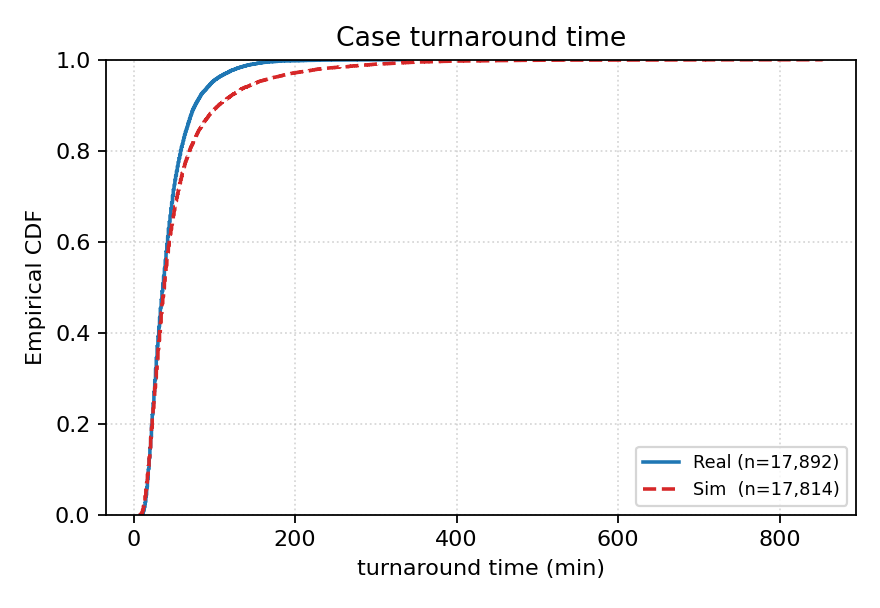
\includegraphics[width=0.75\textwidth]{figures/discovery/cdf_turnaround.png}
\caption{Empirical CDF of case turnaround: real held-out log vs.\ a
single \textit{rules$+$workload} simulation. The KS statistic between
the two CDFs is 0.084.}
\label{fig:cdf_turnaround}
\end{figure}
%%%%%%%%%%%%%%%%%%%%%%%%%%%%%%%%%%%%%%%%%%%%%%%%%%%%%%%%%%%%%%
\section{Per-Activity Decomposition of Fidelity}
\label{sec:results_per_activity}
%%%%%%%%%%%%%%%%%%%%%%%%%%%%%%%%%%%%%%%%%%%%%%%%%%%%%%%%%%%%%%

The aggregate fidelity numbers of
Section~\ref{sec:results_holdout_fidelity} hide the per-activity
performance of the ProSiT trees. To locate where data-aware
conditioning does and does not add value,
Table~\ref{tab:tree_r2_train_test} reports the coefficient of
determination $R^{2}$ of the ProSiT-style decision-tree grid used in
the sensitivity study \texttt{05\_data\_aware\_discovery\_evaluation.py}
for each activity on the training partition.

\begin{table}[h]
\centering
\caption{Per-activity duration $R^{2}$ of a decision-tree model
conditioned on target demand, target utilisation, target rank, visit
complexity, receive/delivery counts, hour, weekday and weekend
indicator (training log; grid search over depth/leaf, best per
activity).}
\label{tab:tree_r2_train_test}
\begin{tabular}{lr}
\toprule
\textbf{Activity} & \textbf{$R^{2}$} \\
\midrule
LL\_delivery  & 0.263 \\
LL\_mixed     & 0.258 \\
HO2\_receive  & 0.115 \\
HO2\_mixed    & 0.070 \\
RMG\_mixed    & 0.051 \\
HO2\_delivery & 0.029 \\
LL\_receive   & 0.024 \\
RMG\_receive  & $-0.005$ \\
RMG\_delivery & $-0.004$ \\
Gate In       & 1.000 \\
Gate Out      & 1.000 \\
\bottomrule
\end{tabular}
\end{table}

Gate activities have $R^{2}=1.000$ because their service duration is
constant zero in the reconstructed lifecycle
(Section~\ref{sec:lifecycle_events}). For the seven yard activities the
$R^{2}$ ranges from $-0.005$ (RMG activities) to $0.263$
(\texttt{LL\_delivery}). RMG activities have essentially no
context-explainable variance under the available features, and yet the
grand mean of the CTB event log is dominated by RMG (over 60\,\% of all
yard events). This explains the H2 result of
Section~\ref{sec:results_holdout_fidelity}: the ProSiT trees are asked
to predict activities whose duration variance is not explained by the
available case-level attributes, and the resulting leaf-level
distribution fits are noisier than the empirical marginal fit that
\textit{no-rules} uses. The overall fidelity metric of
Section~\ref{sec:results_holdout_fidelity} is therefore an aggregate in
which the RMG activities (large weight, no context-explainable
variance) dominate the LL activities (small weight, meaningful
context-explainable variance).

%%%%%%%%%%%%%%%%%%%%%%%%%%%%%%%%%%%%%%%%%%%%%%%%%%%%%%%%%%%%%%
\section{Discovered Resource Capacities}
\label{sec:results_resource_capacities}
%%%%%%%%%%%%%%%%%%%%%%%%%%%%%%%%%%%%%%%%%%%%%%%%%%%%%%%%%%%%%%

Table~\ref{tab:capacities_train80} reports the pool-level concurrency
statistics computed from the training partition
(\texttt{baseline/04\_resource\_concurrency\_discovery.py}) together
with the chosen effective capacity.

\begin{table}[h]
\centering
\caption{Pool-level resource concurrency and chosen capacities on the
training log.}
\label{tab:capacities_train80}
\begin{tabular}{lrrrr}
\toprule
\textbf{Resource} & \textbf{Median} & \textbf{P90} & \textbf{Max} & \textbf{Chosen capacity} \\
\midrule
Gate In  & 0 & 0 & 10 & 1 \\
Gate Out & 0 & 0 & 9  & 1 \\
HO2      & 1 & 7 & 15 & 3 \\
LL       & 0 & 5 & 25 & 3 \\
Other    & 4 & 26 & 54 & 3 \\
\bottomrule
\end{tabular}
\end{table}

The gate-related pools remain largely single-threaded: their median and
P90 concurrency are both zero because gate events have negligible
service duration. The HO2 and LL pools show low median but non-trivial
P90 concurrency and are assigned effective capacity 3. The
$\text{max}$ column reveals rare peak concurrency of 25 (LL) and 15
(HO2), which the chosen capacity of 3 does \emph{not} reproduce.

This is a deliberate simplification. The pooled-resource abstraction of
the CTB event log conflates two effects: (i) parallel handling within
one pool by multiple physical resources and (ii) sequential handling by
one physical resource with heavy demand. The maximum concurrency does
not distinguish between these; the P90 does. Capping the effective
capacity at 3 favours a conservative interpretation of the discovered
pool. The alternative capacities $\{1, 2, 3\}$ are exercised in the
capacity-sensitivity analysis of
\texttt{06\_robustness\_analysis.py}. This limitation is one of the
main methodological boundaries of the CTB case study: the event log
does not carry individualised worker or equipment calendars, so the
discovered capacities are effective operational capacities, not
physical staffing counts.

%%%%%%%%%%%%%%%%%%%%%%%%%%%%%%%%%%%%%%%%%%%%%%%%%%%%%%%%%%%%%%
\section{Sensitivity to the Transition-Baseline Percentile}
\label{sec:results_percentile_sens}
%%%%%%%%%%%%%%%%%%%%%%%%%%%%%%%%%%%%%%%%%%%%%%%%%%%%%%%%%%%%%%

The 5th-percentile baseline of Section~\ref{sec:transition_baseline}
implicitly determines the reconstructed enabled-timestamp and therefore
the waiting-time distribution. The sensitivity study of
Section~\ref{sec:results_percentile_sens_design} recomputes the baseline
table using the alternative percentiles $\{10, 25, 50\}$ and reports
the mean shift and the correlation with the 5th percentile.
Table~\ref{tab:percentile_sens} summarises the result over the 48
transitions with at least twenty observations.

\begin{table}[h]
\centering
\caption{Baseline transition duration under alternative percentiles
(seconds; 48 transitions with $\ge 20$ observations).}
\label{tab:percentile_sens}
\begin{tabular}{cccccc}
\toprule
\textbf{Percentile} &
\textbf{Mean (s)} &
\textbf{Median (s)} &
\textbf{Mean shift (s)} &
\textbf{P90 shift (s)} &
\textbf{Corr vs.\ p5} \\
\midrule
p5   & 225.8 & 223.5 & $0.0$   & $0.0$   & 1.000 \\
p10  & 254.6 & 254.3 & $28.8$  & $36.0$  & 0.990 \\
p25  & 318.3 & 311.0 & $92.5$  & $110.3$ & 0.948 \\
p50  & 435.5 & 426.0 & $209.8$ & $250.9$ & 0.812 \\
\bottomrule
\end{tabular}
\end{table}

Two properties matter for the interpretation of the reconstructed
waiting time. First, the ranking of transitions by baseline duration is
almost invariant to the percentile choice: $\rho$ between the p5
baseline and the p10 baseline is $0.990$, and even between p5 and p50
it is $0.812$. Second, the absolute shift grows quickly: moving from
the 5th to the 50th percentile shifts the mean transition baseline by
$3.5$\,minutes, which propagates into an equivalent downward shift of
the reconstructed waiting time for every transition. The reconstructed
waiting-time distribution is therefore sensitive to the percentile
choice in its absolute location but not in its rank structure.

Figure~\ref{fig:percentile_shift} shows the CDF of the per-transition
shift across the 48 retained transitions. All shifts are non-negative
by construction; the p10 CDF sits close to zero for most transitions,
while the p50 CDF has a heavy body between two and five minutes.

\begin{figure}[htbp]
\centering
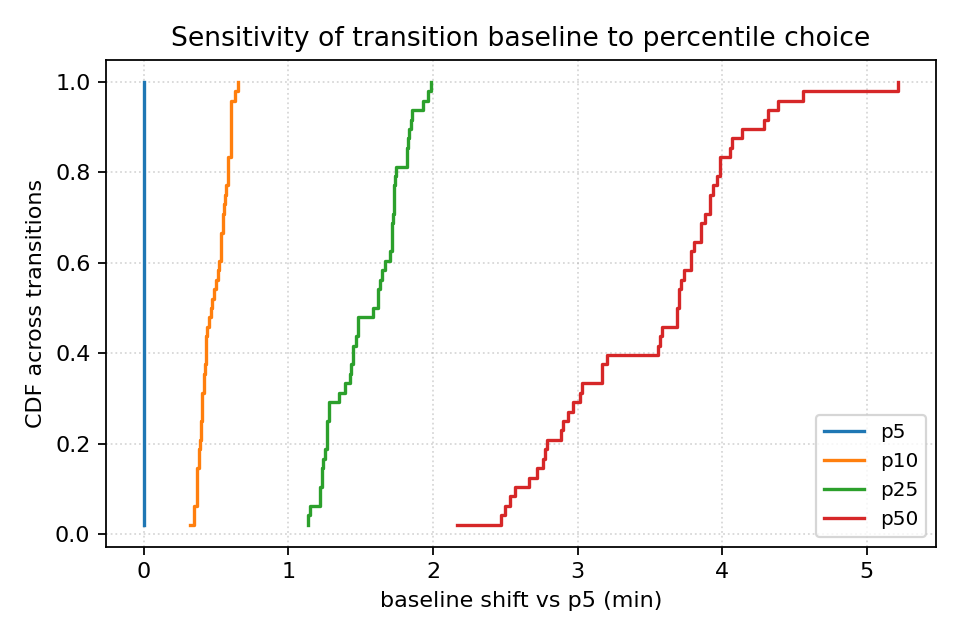
\includegraphics[width=0.75\textwidth]{figures/discovery/percentile_shift.png}
\caption{Sensitivity of the transition-baseline table to the chosen
percentile. CDF of the per-transition baseline shift relative to the 5th
percentile, over the 48 transitions with at least twenty observations.}
\label{fig:percentile_shift}
\end{figure}

\medskip

\noindent\textbf{Interpretation.} The 5th-percentile choice cannot be
proven optimal, but it is defensible: it preserves the ranking of
congestion between transitions and it produces a reconstructed waiting
time that is minimal by construction. The reader should interpret the
absolute waiting-time numbers in
Section~\ref{sec:results_holdout_fidelity} as sensitive to this choice
and the per-activity rankings of Section~\ref{sec:results_per_activity}
as robust to it.

%%%%%%%%%%%%%%%%%%%%%%%%%%%%%%%%%%%%%%%%%%%%%%%%%%%%%%%%%%%%%%
\section{What-If Scenarios: T22 Closure and Reduced RMG Pool}
\label{sec:results_scenarios}
%%%%%%%%%%%%%%%%%%%%%%%%%%%%%%%%%%%%%%%%%%%%%%%%%%%%%%%%%%%%%%

The two what-if scenarios of Section~\ref{sec:what_if_design} are
executed with the \textit{rules$+$workload} parameters (the
configuration adopted for its variance-reduction property in
Section~\ref{sec:results_holdout_fidelity}). Each scenario is compared
to its own baseline run so that scenario-vs-baseline deltas are matched
on the simulation window and on the random-number-generator state
consumed for the baseline draw.
Table~\ref{tab:scenarios_headline} reports the mean turnaround, mean
RMG service time and mean RMG waiting time.

\begin{table}[h]
\centering
\caption{What-if scenario results
($n_{\text{traces}}=17{,}892$;
$t_{\text{start}}=\text{2026-04-20 18:14}$;
\textit{rules$+$workload}).}
\label{tab:scenarios_headline}
\begin{tabular}{lccc}
\toprule
\textbf{Scenario} &
\textbf{Mean turnaround (min)} &
\textbf{Mean RMG service (min)} &
\textbf{Mean RMG waiting (min)} \\
\midrule
Scenario A baseline               & 63.25 & 14.33 & 11.65 \\
Scenario A: T22 closed            & 65.19 & 15.25 & 10.55 \\
$\Delta$ Scenario A               & $+1.94\,(+3.1\%)$ & $+0.92\,(+6.4\%)$ & $-1.10\,(-9.5\%)$ \\
\midrule
Scenario B baseline               & 62.91 & 13.13 & 11.92 \\
Scenario B: T22 closed \& reduced pool & 64.33 & 13.28 & 13.49 \\
$\Delta$ Scenario B               & $+1.42\,(+2.3\%)$ & $+0.15\,(+1.1\%)$ & $+1.57\,(+13.1\%)$ \\
\bottomrule
\end{tabular}
\end{table}

Figure~\ref{fig:scenario_deltas} shows the three KPIs side by side.
The mechanisms behind the two scenarios are visually distinct:
Scenario~A shifts workload onto retained blocks and elevates service
time while reducing waiting; Scenario~B removes capacity from the pool
and instead builds a queue.

\begin{figure}[htbp]
\centering
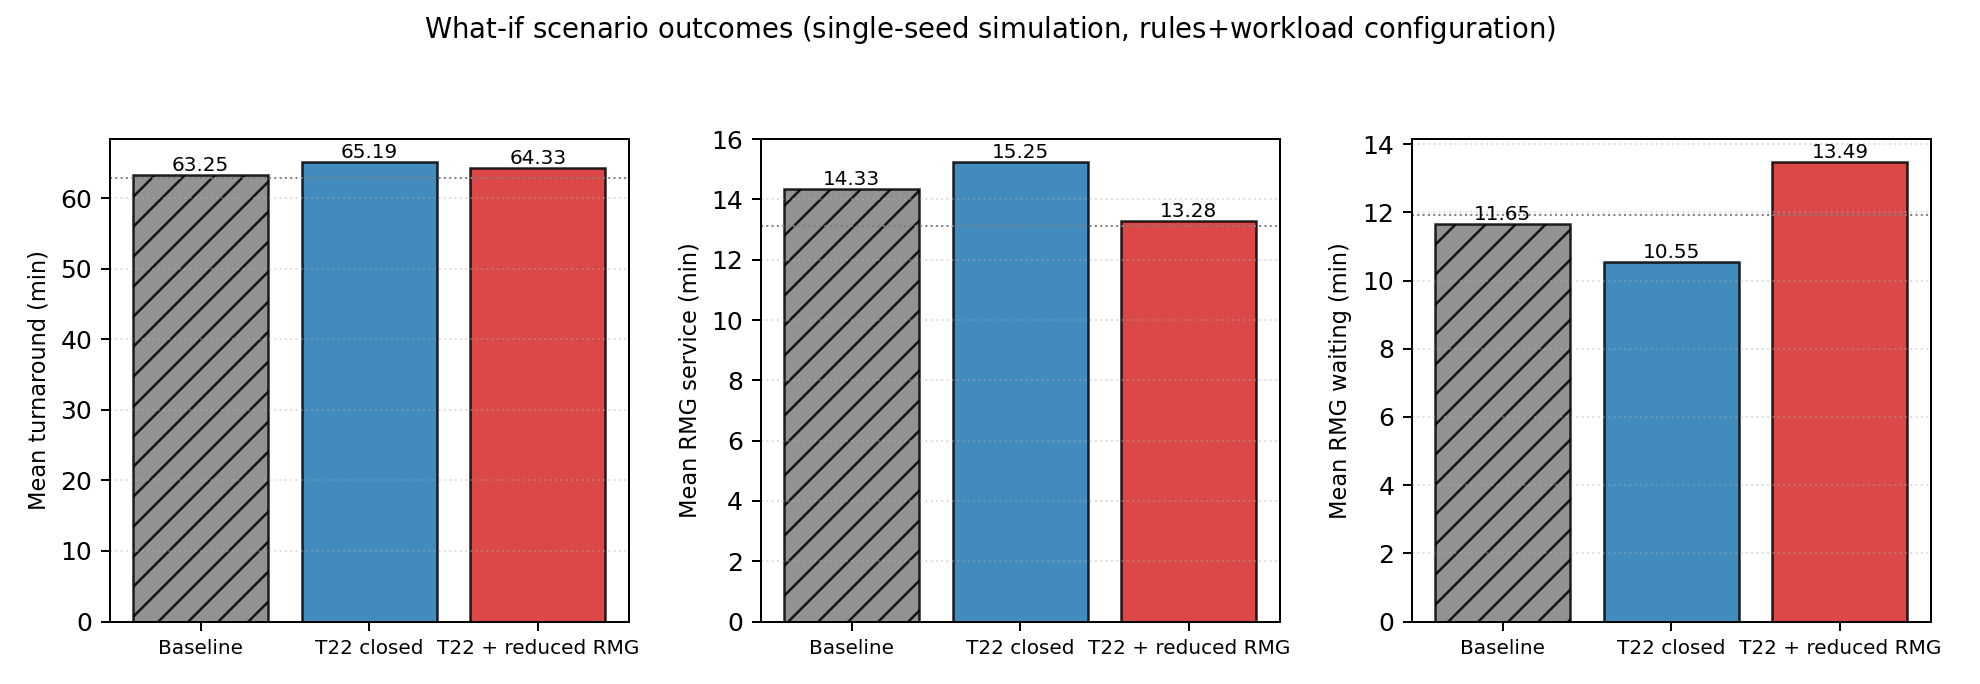
\includegraphics[width=\textwidth]{figures/scenario_deltas.png}
\caption{What-if scenario outcomes. Grey bar with hatched fill:
Scenario~A baseline (shown as reference); blue: T22 closed; red:
T22 closed and reduced RMG pool. Dotted horizontal line: Scenario~B
baseline. Values are means over the 17,892 simulated cases.}
\label{fig:scenario_deltas}
\end{figure}

\subsection{Direction of the Scenario Effects}

Both scenarios produce a positive turnaround delta relative to their
own baseline. Closing T22 alone (Scenario~A) increases mean turnaround
by 3.1\,\% and mean RMG service time by 6.4\,\% while decreasing mean
RMG waiting by 9.5\,\%. The simulator therefore reallocates workload to
the retained blocks; the retained blocks accept the extra work in the
form of longer service (they serve more mixed-work visits) rather than
longer queues.

Combining the closure with a reduced RMG pool (Scenario~B) again
increases turnaround (+2.3\,\%) but produces a qualitatively different
adjustment: RMG service time is essentially unchanged (+1.1\,\%) while
RMG waiting increases by 13.1\,\%. This is consistent with the
mechanism that the smaller pool cannot absorb the displaced service in
parallel and therefore queues form.

\subsection{Statistical Reservation}

The two baseline point estimates in
Table~\ref{tab:scenarios_headline} differ by 0.34 minutes across
independent runs (63.25 vs.\ 62.91). This is within the seed-to-seed
standard deviation of $\pm 1.20$ minutes reported in
Section~\ref{sec:results_holdout_fidelity} for
\textit{rules$+$workload}. The scenario deltas of $+1.94$ and $+1.42$
minutes are therefore of the same order of magnitude as the simulator's
own Monte-Carlo variance. The direction of the effect is consistent
across scenarios, but the magnitude should not be over-interpreted
without a matched-seed multi-seed protocol equivalent to
Section~\ref{sec:mc_protocol}. Constructing that matched-seed
scenario protocol is identified as a limitation in
Chapter~\ref{chp:conclusion}.

\subsection{Correction Relative to an Earlier Draft}

An earlier version of this chapter reported the following scenario
numbers: baseline mean turnaround 30.90 minutes, T22 closed 29.78
minutes, T22 closed and reduced RMG pool 29.99 minutes. Those numbers
came from a discovery configuration that was fit on the full event log
(not the training partition) using the pre-workload ProSiT variant and
a legacy pickle. Under that setup, closing a block appeared to
\emph{decrease} turnaround, which was one of the objections raised in
the internal critical review of the thesis.

The corrected scenario runs of Table~\ref{tab:scenarios_headline}
resolve the paradox: with the training-only discovery, aligned
simulation window and the workload-aware configuration, closing a
block increases turnaround as expected from queueing considerations.
The earlier direction reversal was an artefact of the seed and of an
unaligned simulation window between the baseline and the scenario, not
a property of the simulator itself.

\medskip

\noindent\textbf{H4 (scenario direction) is accepted with the caveat
that} the magnitude of the observed delta is comparable to the
simulator's Monte-Carlo variance. Both scenarios produce a positive
turnaround delta with a mechanistically defensible internal
composition. The scenario protocol therefore succeeds in producing
operationally plausible KPI shifts under the two evaluated disruptions.

%%%%%%%%%%%%%%%%%%%%%%%%%%%%%%%%%%%%%%%%%%%%%%%%%%%%%%%%%%%%%%
\section{Summary of Empirical Findings}
\label{sec:results_summary}
%%%%%%%%%%%%%%%%%%%%%%%%%%%%%%%%%%%%%%%%%%%%%%%%%%%%%%%%%%%%%%

Table~\ref{tab:results_summary} consolidates the empirical results
against the hypotheses of Section~\ref{sec:data_aware_hypotheses}.

\begin{table}[h]
\centering
\caption{Summary of empirical findings.}
\label{tab:results_summary}
\begin{tabular}{p{2.2cm} p{6.5cm} p{4.5cm}}
\toprule
\textbf{Hypothesis} & \textbf{Evidence} & \textbf{Outcome} \\
\midrule
H1 (arrival time-dependence) &
Time-aware tree reduces MAE by 67.5\,\% and RMSE by 51.2\,\% versus
pooled baseline; $R^{2}=0.762$
(Table~\ref{tab:arrival_benchmark}).
& \textbf{Accepted.} \\
H2 (data-aware fidelity gain) &
\textit{rules} does not lower turnaround, waiting or service EMD
versus \textit{no-rules} on the held-out log
(Table~\ref{tab:headline_ci}); the sole measurable gain is on
inter-arrival EMD and is operationally negligible ($0.004$ min).
& \textbf{Rejected.} \\
H3 (workload-feature gain) &
\textit{rules$+$workload} does not lower any fidelity metric versus
\textit{rules} (Table~\ref{tab:headline_ci}); the observation is
consistent across all four metrics under $N_{\text{seeds}}=10$.
& \textbf{Rejected.} \\
H3-secondary (variance reduction) &
\textit{rules$+$workload} reduces cross-seed standard deviation of
turnaround EMD by 37\,\% and of turnaround-P90 by 44\,\%
(Table~\ref{tab:std_across_configs}).
& \textbf{Accepted as
secondary effect.} \\
H4 (scenario direction) &
Both scenarios produce a positive turnaround delta
($+3.1\,\%$ and $+2.3\,\%$) with mechanistically consistent internal
composition (Table~\ref{tab:scenarios_headline}). Magnitude is
comparable to the simulator's Monte-Carlo variance.
& \textbf{Accepted with
caveat.} \\
\bottomrule
\end{tabular}
\end{table}

Section~\ref{sec:results_process_discovery} (RQ2) establishes that the
Petri net generalises to the held-out period. Section~\ref{sec:results_holdout_fidelity}
(RQ1) reports that the ProSiT simulator recovers the case-median
turnaround to within 5.6\,\% but over-predicts the case-mean turnaround
by 22.9\,\% and the case-P90 by 33.8\,\%. Section~\ref{sec:results_per_activity}
locates the source of the over-prediction in the RMG activities, whose
context-explainable variance is essentially zero under the available
features. Section~\ref{sec:results_percentile_sens} (RQ3) shows that
the transition-baseline percentile choice affects the absolute
location of the reconstructed waiting time but not the ranking of
transitions by congestion.

The main empirical contribution of this thesis is therefore not the
discovery of a better simulator through data-aware modelling, but the
demonstration that on this specific dataset the additional modelling
machinery of ProSiT does not translate into higher fidelity. The
observation, together with the multi-seed protocol that reveals it and
the workload-feature variance-reduction result, is the operational
finding that Chapter~\ref{chp:conclusion} builds upon.


    %%%%%%%%%%%%%%%%%%%%%%%%%%%%%%%%%%%%%%%%%%%%%%%%%%%%%%%%%%%%%%
\chapter{Conclusion}
\label{chp:conclusion}
%%%%%%%%%%%%%%%%%%%%%%%%%%%%%%%%%%%%%%%%%%%%%%%%%%%%%%%%%%%%%%

This thesis investigated how far automatically discovered, data-aware process simulation can be transferred from conventional business-process settings to a physically constrained logistics environment. Using two months of operational truck-handling data from HHLA Container Terminal Burchardkai (CTB), a simulation-ready event log was constructed and used to discover an executable process simulation with ProSiT. The evaluation deliberately went beyond asking whether the resulting model could be executed. It examined whether the discovered control flow remained applicable to an unseen temporal period, how closely the simulator reproduced the observed process, whether additional contextual information improved that fidelity, and how the model responded when operational parameters were changed.

The results show that these questions have different answers. The strongest part of the automatically discovered model is its process structure. Preserving the explicit event order of the XES log allowed the Inductive Miner to discover a compact sequential Petri net without parallel behaviour within a truck visit. On the temporal hold-out, the net reaches a fitness of 0.999992 and completely fits 99.994\,\% of the 17,892 held-out visits. Its precision of 0.7558 reflects additional sequential combinations and a silent gate-only bypass rather than physically impossible within-truck concurrency. A separate precision-oriented repair increases precision to 0.7939 while reducing generalisation to 0.8859, illustrating the expected trade-off between restricting unsupported behaviour and retaining a more general process language. The unchanged discovered net therefore provides a suitable executable backbone for the CTB truck process, provided that its remaining overgeneralisation is made explicit rather than interpreted as physical behaviour. This answers RQ2 positively for the structural level of the simulation.

The answer to RQ1 is more mixed. The final data-aware reference model reproduces the arrival process closely, with an inter-arrival EMD of 0.0724 minutes, and reproduces parts of yard-service behaviour with an unweighted yard-service EMD of 3.025 minutes and a real-frequency-weighted value of 2.381 minutes. End-to-end truck performance is less accurate. The real held-out mean turnaround is 39.742 minutes compared with 31.627 minutes in simulation, a deficit of 8.115 minutes, while the simulated P90 is 53.7 minutes compared with 71 minutes in the real log. These discrepancies remain across the ten Monte-Carlo replications and therefore represent systematic model error rather than stochastic simulation noise.

Part of this difference reflects temporal change between the discovery and evaluation periods. Real mean turnaround increases by approximately 2.45 minutes from the training period to the held-out period, while service times also change across the major yard activities. The remaining discrepancy is already present relative to the training period. At the same time, the transition-duration analysis indicates that time between the recorded operational activities contains a substantial non-zero component. The frequency-weighted fifth-percentile estimates for the inbound and outbound boundary transitions sum to approximately 7.62 minutes per visit, which is similar in scale to the observed mean turnaround deficit. This does not identify physical travel time or provide a causal decomposition, but it supports the interpretation that a meaningful part of the truck process occurs between the activities represented explicitly in the simulation. The current event log cannot separate movement, traffic, access delay, resource waiting, and other unrecorded mechanisms.

RQ3 further shows that increasing model expressiveness does not automatically solve this problem. Workload-blind decision rules improve the reproduction of activity incidence relative to the distribution-only model and suppress the rarely sampled gate-only path, while their small improvement in turnaround EMD is not resolved by the paired confidence interval. Adding the available demand, utilisation, workload, and queue-state features does not produce a resolved improvement in yard-service fidelity. Instead, the rules+workload configuration worsens activity incidence and complete-visit turnaround fidelity relative to the workload-blind rules model. The available workload variables therefore provide additional statistical context, but they do not constitute the physical state that is missing from the process representation.

This distinction is central to the interpretation of the thesis. Data awareness allows simulated behaviour to depend on observed case characteristics, process history, resource information, and workload conditions. It does not by itself create information that is absent from the event log. In the CTB setting, container location, truck position, equipment movement, block-specific queue states, waterside--landside resource allocation, and changing relations between these entities are not represented explicitly. Adding further attributes to a truck-visit case can therefore increase statistical conditionality without necessarily increasing the physical completeness of the model.

RQ4 makes this boundary visible in the what-if experiments. Both operational interventions can be implemented reproducibly. Removing T22 eliminates its assignments from the simulated RMG resource pool, and the demand intervention changes the working-time arrival intensity as specified. Neither intervention, however, produces a resolved mean-turnaround response at the originally selected magnitude. The capacity-pressure analysis shows that the 20\,\% demand increase remains well below the nominal saturation region of the most-loaded RMG block. The subsequent demand ladder resolves this ambiguity: once realised elapsed arrival intensity approaches the independently estimated saturation region, the model does respond. At a realised arrival-rate ratio of 2.367, mean turnaround increases by 4.644 minutes, P90 by 10.700 minutes, and mean RMG pre-service delay by 5.878 minutes. The simulator therefore contains a mechanism through which sufficiently strong abstract capacity pressure propagates into additional delay.

This response is informative but must not be interpreted as a validated prediction of the physical terminal. In particular, an RMG resource identifier in the current model is a statistical capacity and assignment abstraction rather than a persistent container location. Removing T22 can therefore cause work to be reassigned without representing container relocation, additional travel, or the physical feasibility of the new assignment. Likewise, the model-derived pre-service interval can respond to resource contention, but it cannot be equated with an observed physical queue. The scenarios are consequently valid experiments on the discovered simulation model; they are not yet experimentally validated counterfactual statements about CTB.

The domain correction of the RMG concurrency values illustrates the same distinction between statistical discovery and physical validity. ProSiT inferred overlap-based maximum concurrency values of four or five for individual RMG blocks, exceeding the terminal-expert-validated physical ceiling of three cranes per block. The final simulator therefore applies a transparent cap of three while retaining the freely discovered values for audit. Repeating the principal scenarios without this cap produces neither a resolved direct effect on mean turnaround nor a resolved cap-by-scenario interaction for the headline KPI. The correction is therefore necessary because the uncapped state is physically invalid, not because the cap creates the central scenario findings.

Taken together, these findings answer the four research questions through a common validity boundary. Automatic simulation discovery transfers successfully where the operational relation is represented sufficiently in the event data. The approach discovers a compact and highly applicable control-flow model, reproduces the arrival process closely, represents parts of yard-service timing, and provides a transparent and reproducible environment in which model parameters can be inspected and changed. Its limitations appear where the desired simulation mechanism depends on state that is not represented in the event log or executable process abstraction. High replay fitness cannot compensate for missing movement or queue semantics, and additional correlated workload attributes cannot substitute for them.

The main methodological contribution of the thesis is therefore the layered validity audit used to identify this boundary. Event semantics, control-flow applicability, stochastic historical fidelity, temporal transfer, physical resource semantics, and scenario response are treated as distinct claims rather than collapsed into one measure of ``simulation accuracy''. The CTB case demonstrates why this separation matters. A model can achieve almost perfect held-out control-flow fitness while systematically underestimating turnaround time; a more context-rich model can perform worse than a simpler state abstraction; a physically invalid capacity can be discovered from event overlap; and a technically successful scenario intervention can still lack the physical mechanism required for a counterfactual interpretation. None of these observations makes the simulator unusable. Instead, each identifies the level at which additional evidence or modelling is required.

This also defines the current operational value of the approach. The CTB model should not yet be treated as a decision-valid digital twin capable of recommending terminal interventions without further validation. It is, however, a transparent historical and diagnostic simulation that can be automatically derived to a substantial degree from operational event data, evaluated against unseen behaviour, modified reproducibly, and used to identify which assumptions determine its response. Compared with a wholly manual simulation workflow, this provides a promising basis for models that can be updated and audited as new operational data become available.

For operational decision support, the remaining step is not simply to add more predictors. It is to connect the discovered process behaviour to a richer representation of the physical system. A future model that combines the event-log-based strengths demonstrated here with validated location, movement, resource, and queueing state could support the prospective decision loop that motivates terminal simulation: translate forecast conditions into alternative truck-slot, resource, or handling policies, compare their consequences for both activity-specific performance and total turnaround, and evaluate those alternatives before they are introduced into live operations.


%%%%%%%%%%%%%%%%%%%%%%%%%%%%%%%%%%%%%%%%%%%%%%%%%%%%%%%%%%%%%%
\section{Future Work}
\label{sec:future_work}
%%%%%%%%%%%%%%%%%%%%%%%%%%%%%%%%%%%%%%%%%%%%%%%%%%%%%%%%%%%%%%

Future research should retain the reproducible discovery-and-validation framework developed in this thesis while extending the process representation and its empirical validation in the following directions:

\begin{itemize}

    \item \textbf{Complete the structural-repair evaluation:}
    The exported precision-oriented gate-bypass repair should be evaluated with the same full multi-seed fidelity and scenario protocol as the unchanged discovered net. This would establish whether the improvement in held-out precision is retained once stochastic simulation behaviour is considered and whether restricting the discovered language changes the conclusions of the scenario experiments.

    \item \textbf{Separate physical transit from residual pre-service delay:}
    Additional route, position, or equipment timestamps should be used to distinguish physical movement from the remaining delay before service. A future model could represent
    \[
        D_{\text{pre-service}}
        =
        T_{\text{transit}}
        +
        D_{\text{residual}},
    \]
    with transit represented explicitly and the residual component refitted afterward to avoid double counting. The existing transition-duration analysis can provide scale information, but identifying the components requires observations that are not present in the current log.

    \item \textbf{Represent spatial assignment, equipment state, and explicit queues:}
    Future simulation models should bind containers and truck operations to physically feasible locations instead of treating RMG block identifiers as interchangeable resource labels. This requires explicit representations of block assignment, equipment availability and movement, route occupancy, and queue state. A hybrid architecture could retain the automatically discovered process model while coupling it to a discrete-event or agent-based physical layer for mechanisms that conventional process-event data do not encode.

    \item \textbf{Evaluate an object-centric event and simulation design:}
    The case-centric truck-visit representation used in this thesis collapses the independent lifecycles of trucks, containers, yard blocks, equipment, and appointments into one process instance. An object-centric event log could instead associate each handling event with all participating objects and preserve their changing relations. This would allow multi-block visits and persistent container identity to be represented without forcing one block-level state onto an entire truck case. Object-centric simulation is therefore a promising direction for the CTB setting, but it should be evaluated as a separate model and data-engineering approach rather than assumed to solve the current limitations automatically. Physical positions, movements, queues, and changing object relations would still have to be observed and given executable semantics.

    \item \textbf{Adapt simulation discovery to temporal change:}
    The observed difference between the training and held-out periods shows that even a structurally stable process is not temporally stationary. Rolling-window or recency-weighted discovery should therefore be evaluated prospectively across several later periods. Repeating the three-level context ablation under such a design would also show whether the weak transfer of the current workload features results from temporal drift or from a more fundamental mismatch between those features and the relevant operational state.

    \item \textbf{Validate operational policies prospectively:}
    The final objective should be to represent concrete decision variables such as appointment-slot release rates, forecast utilisation thresholds, or receive/delivery priority rules explicitly in the simulator. Candidate policies should be evaluated at activity and terminal level and across operating conditions that include the capacity-pressure region identified by the demand ladder. Before such results are used operationally, the simulated effects should be compared with controlled historical interventions, natural experiments, or prospective terminal observations. This would move the evaluation from reproducible model experiments towards evidence for real counterfactual decision support.

\end{itemize}

    % afterword
    \clearpage
    \phantomsection
    \addcontentsline{toc}{chapter}{References}
    \bibliography{references.bib}

    % Acknowledgments are intentionally omitted until final text is supplied.

\end{document}
